\documentclass[12pt,a4paper,oneside]{book}
\usepackage[utf8]{inputenc}
\usepackage{tabularx}

\usepackage{amsmath}
\usepackage{amsfonts}
\usepackage{amssymb}
\usepackage[spanish]{babel}
\usepackage{graphicx}
\usepackage{wrapfig}
\usepackage{fancyhdr}
\usepackage[hidelinks]{hyperref}
\usepackage{datatool}
\usepackage[acronym]{glossaries}
%\usepackage[style=glossary,backend=bibtex]{biblatex}
% acronyms
%\usepackage{acronym} 

\usepackage{makeidx}
\usepackage{multirow}
\usepackage{multicol}
\usepackage{colortbl}
\usepackage{cite}
\usepackage{float}
 \usepackage{comment} 

\makeindex
\pagestyle{fancy}
\fancyhf{} % Clear all header and footer fields
\fancyfoot[C]{\thepage} % Center the page number at the bottom

%\addbibresource{glosario.bib}

\makeglossaries % este comando debe estar en el preámbulo

% \fancyhead{}
% \fancyfoot{}


% % \lhead{Glosario}
% % \begin{LARGE}
% % \textbf{Glosario}
% % \end{LARGE}

% % \lhead{Glosario.}
% % %\rhead{\today}
% % %\rfoot{\thepage}

% % \chapter{Glosario}

\newglossaryentry{nwkskey-glossary}{
    name={Network Session Key},
    description={Clave de cifrado utilizada en LoRaWAN para proteger la comunicación entre el dispositivo final y el servidor de red, garantizando la autenticidad y la integridad de los datos transmitidos.}
}
\newacronym{nwkskey-acronym}{NwkSKey}{Clave de Sesión de Red}

\newacronym{appskey-acronym}{AppSKey}{Clave de Sesión de Aplicación}
\newglossaryentry{appskey-glossary}{
    name={Application Session Key},
    description={Clave de cifrado utilizada en LoRaWAN para garantizar la confidencialidad de los datos entre el dispositivo final y el servidor de aplicación.}
}

\newacronym{appkey-acronym}{AppKey}{Application Key (Clave de Aplicación)}





\newacronym{adr-acronym}{ADR}{Tasa de Datos Adaptativa}
\newglossaryentry{adr-glossary}{
    name={Adaptive Data Rate},
    description={Mecanismo en LoRaWAN que ajusta automáticamente la velocidad de transmisión de datos y la potencia según las condiciones de la señal.}
}



\newacronym{wsn-acronym}{WSN}{redes de sensores inalámbricos}
\newglossaryentry{wsn-glossary}{
    name={wireless sensor networks},
    description={Mecanismo en LoRaWAN que ajusta automáticamente la velocidad de transmisión de datos y la potencia según las condiciones de la señal.}
}

\newacronym{ism-acronym}{ISM}{Industrial, Scientific, and Medical (Banda Industrial, Científica y Médica)}

\newglossaryentry{ism-glossary}{
    name={Industrial, Scientific, and Medical},
    description={Conjunto de bandas de frecuencia de radio designadas a nivel mundial para el uso de equipos industriales, científicos y médicos, así como para tecnologías inalámbricas como Wi-Fi, Bluetooth y LoRa.}
}



\newacronym{lpwan-acronym}{LPWAN}{ (Red de Área Amplia de Bajo Consumo)}


\newglossaryentry{aes}{name={Advanced Encryption Standard},description={Estándar de cifrado avanzado utilizado para asegurar la transmisión de datos en redes como LoRaWAN.}}

\newacronym{aes-acronym}{AES}{Estándar de Cifrado Avanzado}

\newglossaryentry{rtos}{name={FreeRTOS},description={Sistema operativo en tiempo real para microcontroladores y pequeños microprocesadores.}}

\newglossaryentry{api}{name={Application Programming Interface},description={Conjunto de herramientas y definiciones que permiten la interacción entre aplicaciones de software.}}
% \newglossaryentry{arduino}{name={Arduino},description={Plataforma de hardware y software abierta para el desarrollo de proyectos electrónicos y de programación.}}
\newglossaryentry{ble}{name={Bluetooth Low Energy},description={Tecnología de comunicación inalámbrica diseñada para bajo consumo energético.}}
% \newglossaryentry{base64}{name={Base64},description={Codificación de texto para representar datos binarios, utilizada comúnmente para transmitir datos de manera segura.}}
\newglossaryentry{cmac}{name={Cipher-based Message Authentication Code},description={Método para asegurar la integridad y autenticidad de mensajes cifrados.}}

\newacronym{cmac-acronym}{CMAC}{Código de Autenticación de Mensaje basado en Cifrado}


\newglossaryentry{css}{name={Chirp Spread Spectrum},description={Técnica de modulación utilizada en LoRa para transmitir datos a largas distancias con baja potencia.}}

\newacronym{css-acronym}{CSS}{Espectro Ensanchado de Chirp}


\newglossaryentry{fhss}{name={Frequency-Hopping Spread Spectrum},description={Tecnología que cambia frecuentemente la frecuencia de transmisión para evitar interferencias.}}
\newglossaryentry{fsk}{name={Frequency Shift Keying},description={Método de modulación para transmitir datos digitales mediante cambios en la frecuencia de la señal portadora.}}
\newglossaryentry{freertos}{name={FreeRTOS},description={Sistema operativo en tiempo real utilizado en microcontroladores para gestionar múltiples tareas de manera eficiente.}}
\newglossaryentry{glonass}{name={Global Navigation Satellite System},description={Sistema ruso de navegación por satélite que complementa al GPS.}}
\newglossaryentry{gnss}{name={Global Navigation Satellite System},description={Término genérico para sistemas de posicionamiento global que incluyen GPS, GLONASS, entre otros.}}
\newglossaryentry{gps}{name={Global Positioning System},description={Sistema de navegación por satélite que proporciona datos de localización precisos.}}
\newglossaryentry{gsm}{name={Global System for Mobile Communications},description={Tecnología de comunicación móvil utilizada para voz y datos.}}
\newglossaryentry{iot}{name={Internet of Things},description={Red de dispositivos interconectados que recopilan y comparten datos en tiempo real para automatizar procesos.}}
\newglossaryentry{json}{name={JavaScript Object Notation},description={Formato ligero para el intercambio de datos, fácil de leer y escribir.}}
\newglossaryentry{lte}{name={Long Term Evolution},description={Tecnología de redes móviles de alta velocidad.}}
\newglossaryentry{lorawan}{name={Long Range Wide Area Network},description={Protocolo de red para dispositivos IoT que permite transmisiones de datos de largo alcance y bajo consumo.}}
\newglossaryentry{mac}{name={Media Access Control},description={Identificador único para dispositivos de red en comunicaciones.}}

\newacronym{mac-acronym}{MAC}{Control de Acceso al Medio}

\newglossaryentry{backhaul-glossary}{
    name={Backhaul},
    description={Segmento de la red que conecta los nodos de acceso (como estaciones base o gateways) a la red principal o al backbone, permitiendo la transmisión de datos de manera eficiente.}
}


\newglossaryentry{miso}{name={Master In Slave Out},description={Línea de datos utilizada en comunicación SPI.}}
\newglossaryentry{mosi}{name={Master Out Slave In},description={Línea de datos utilizada en comunicación SPI.}}
\newglossaryentry{mqtt}{name={Message Queuing Telemetry Transport},description={Protocolo ligero para la transmisión de mensajes entre dispositivos IoT.}}
\newglossaryentry{nfc}{name={Near Field Communication},description={Tecnología inalámbrica de corto alcance utilizada en pagos móviles y autenticación.}}
\newglossaryentry{otaa}{name={Over-The-Air Activation},description={Método de activación de dispositivos LoRaWAN para generar claves de sesión de forma dinámica.}}
\newglossaryentry{rfid}{name={Radio Frequency Identification},description={Tecnología de identificación y seguimiento mediante ondas de radio.}}
\newglossaryentry{spi}{name={Serial Peripheral Interface},description={Protocolo de comunicación serial para dispositivos embebidos.}}
\newglossaryentry{sx1262}{name={SX1262},description={Chip de comunicación LoRa utilizado en aplicaciones IoT.}}
\newglossaryentry{tdoa}{name={Time Difference of Arrival},description={Técnica para determinar la ubicación de un dispositivo mediante la diferencia de tiempo en la llegada de señales.}}
\newglossaryentry{thingsboard}{name={ThingsBoard},description={Plataforma de gestión de dispositivos IoT y visualización de datos en tiempo real.}}
\newglossaryentry{uart}{name={Universal Asynchronous Receiver-Transmitter},description={Protocolo para la comunicación serial asíncrona entre dispositivos.}}

\newacronym{rssi-acronym}{RSSI}{Indicador de Intensidad de Señal Recibida}

\newacronym{toa-acronym}{TOA}{Time on Air (Tiempo en el Aire)}
\newglossaryentry{toa-glossary}{
    name={Time on Air},
    description={Duración total que un mensaje ocupa en el medio de transmisión durante su envío, calculado en función del tamaño del mensaje, el factor de dispersión (SF), el ancho de banda y otros parámetros. Es un indicador clave en LoRaWAN.}
}
\newacronym{i2s-acronym}{I2S}{Inter-IC Sound (Interconexión de Circuitos Integrados de Sonido)}

\newacronym{i2c-acronym}{I2C}{Inter-Integrated Circuit (Interconexión de Circuitos Integrados)}

\newacronym{lns-acronym}{LNS}{LoRaWAN Network Server (Servidor de Red LoRaWAN)}
\newglossaryentry{lns-glossary}{
    name={LoRaWAN Network Server},
    description={Componente central en una red \gls{lorawan-glossary} que gestiona la autenticación, la enrutación de datos, y el control de dispositivos finales. Coordina las comunicaciones entre gateways y aplicaciones.}
}



% Acrónimos
\newacronym{loraw}{LoRaWAN}{Red de Área Amplia de Largo Alcance}
\newacronym{rf}{RF}{Radiofrecuencia}
\newacronym{iot-acronym}{IoT}{Internet de las Cosas}
\newacronym{rfid-acronym}{RFID}{Identificación por Radiofrecuencia}
\newacronym{gps-acronym}{GPS}{Sistema de Posicionamiento Global}
\newacronym{gnss-acronym}{GNSS}{Sistema Global de Navegación por Satélite}
\newacronym{lora-acronym}{LoRa}{Largo Alcance}
\newacronym{uart-acronym}{UART}{Universal Asynchronous Receiver-Transmitter (Receptor-Transmisor Asíncrono Universal)}
\newacronym{spi-acronym}{SPI}{Serial Peripheral Interface (Interfaz Periférica Serial)}
\newacronym{api-acronym}{API}{Application Programming Interface (Interfaz de Programación de Aplicaciones)}
\newacronym{json-acronym}{JSON}{JavaScript Object Notation (Notación de Objetos de JavaScript)}
\newacronym{gsm-acronym}{GSM}{Global System for Mobile Communications (Sistema Global para Comunicaciones Móviles)}

\newacronym{sms-acronym}{SMS}{Short Message Service (Servicio de Mensajes Cortos)}




\newacronym{otaa-acronym}{OTAA}{Activación por el Aire}
\newacronym{ble-acronym}{BLE}{Bluetooth Low Energy (Bluetooth de Baja Energía)}
\newacronym{fhss-acronym}{FHSS}{Frequency-Hopping Spread Spectrum (Espectro Ensanchado por Salto de Frecuencia)}
\newacronym{nfc-acronym}{NFC}{Near Field Communication (Comunicación de Campo Cercano)}
\newacronym{lte-acronym}{LTE}{Long Term Evolution (Evolución a Largo Plazo)}

% Glosario
\newglossaryentry{iot-glossary}{name={Internet of Things},description={Red de dispositivos interconectados que recopilan y comparten datos en tiempo real para automatizar procesos.}}
\newglossaryentry{rfid-glossary}{name={Radio Frequency Identification},description={Tecnología de identificación y seguimiento mediante ondas de radio.}}
\newglossaryentry{gps-glossary}{name={Global Positioning System},description={Sistema de navegación por satélite que proporciona datos de localización precisos.}}
\newglossaryentry{gnss-glossary}{name={Global Navigation Satellite System},description={Término genérico para sistemas de posicionamiento global que incluyen GPS, GLONASS, entre otros.}}
\newglossaryentry{lorawan-glossary}{name={Long Range Wide Area Network},description={Protocolo de red para dispositivos IoT que permite transmisiones de datos de largo alcance y bajo consumo.}}
\newglossaryentry{uart-glossary}{name={Universal Asynchronous Receiver-Transmitter},description={Protocolo para la comunicación serial asíncrona entre dispositivos.}}
\newglossaryentry{spi-glossary}{name={Serial Peripheral Interface},description={Protocolo de comunicación serial para dispositivos embebidos.}}
\newglossaryentry{api-glossary}{name={Application Programming Interface},description={Conjunto de herramientas y definiciones que permiten la interacción entre aplicaciones de software.}}
\newglossaryentry{json-glossary}{name={JavaScript Object Notation},description={Formato ligero para el intercambio de datos, fácil de leer y escribir.}}
\newglossaryentry{gsm-glossary}{name={Global System for Mobile Communications},description={Tecnología de comunicación móvil utilizada para voz y datos.}}

\newglossaryentry{otaa-glossary}{name={Over-The-Air Activation},description={Método de activación de dispositivos LoRaWAN para generar claves de sesión de forma dinámica.}}
\newglossaryentry{ble-glossary}{name={Bluetooth Low Energy},description={Tecnología de comunicación inalámbrica diseñada para bajo consumo energético.}}
\newglossaryentry{fhss-glossary}{name={Frequency-Hopping Spread Spectrum},description={Tecnología que cambia frecuentemente la frecuencia de transmisión para evitar interferencias.}}
\newglossaryentry{nfc-glossary}{name={Near Field Communication},description={Tecnología inalámbrica de corto alcance utilizada en pagos móviles y autenticación.}}
\newglossaryentry{lte-glossary}{name={Long Term Evolution},description={Tecnología de redes móviles de alta velocidad.}}



\begin{document}
\renewcommand{\glossaryname}{Glosario}
\renewcommand\listtablename{Índice de Tablas}
\renewcommand{\tablename}{Tabla}
\renewcommand{\acronymname}{Acrónimos y símbolos}
\renewcommand{\bibname}{Referencias bibliográficas}

\frontmatter
\pagenumbering{roman}
\pagestyle{plain} % Número de páginas estilo plain para el frontmatter
%%desdeaca
%\frontmatter
\vspace*{-3cm}
\begin{figure}[h]
\leavevmode
\begin{minipage}{\textwidth}
\begin{center}
%\includegraphics[scale=0.5]{./logofpune}
\end{center}
\end{minipage}
\end{figure}

\thispagestyle{empty}

{\bf
\begin{center}
\large
\vspace*{-1 cm}\Large \textsc{Universidad Nacional del Este.} \\
\Large \textsc{Facultad Politécnica.} \\
\vspace*{0.5 cm}\hrule
\end{center}
}

\vspace*{-0.5 cm}
\begin{figure}[htb]
\begin{center}

\includegraphics[scale = 0.6]{./portada_y_ficha_catalografica/logo.png}

\end{center}
\end{figure}


\vspace{3 cm}
{
\noindent
\begin{center}
\huge \bf Sistema de rastreo e
identificación para motocicletas
empleando tecnología IoT.
\end{center}
}


\vspace{5 cm}

\begin{center}
{\textbf{\Large José Mario Barreto Jara.}\\[5mm]
\textbf{\Large Mackey Ryuto Sugawara Mochinaga.}\\[5mm]
\vspace{1 cm}
\textbf{Año \the\year.}}
\end{center}
%%cierre


\vspace*{-3cm}
\begin{figure}[h]
\leavevmode
\begin{minipage}{\textwidth}
\begin{center}
%
\includegraphics[scale=0.5]{./logo}
\end{center}
\end{minipage}
\end{figure}

\thispagestyle{empty}

{\bf
\begin{center}
\large
\vspace*{-1 cm}\Large \textsc{Universidad Nacional del Este.} \\
\Large \textsc{Facultad Politécnica.} \\
\vspace*{0.5 cm}\hrule
\vspace*{0.5 cm}\Large Carrera Ingeniería de Sistemas.\\
\vspace*{0 cm}\Large Cátedra Trabajo Final de Grado.\\
\end{center}
}

\vspace{3.5 cm}
{
\noindent
\begin{center}
\huge \bf  Sistema de rastreo e identificación para motocicletas empleando tecnología IoT.
\end{center}
}


\vspace{0.5 cm}
{ 

Por: \textbf{\Large José Mario Barreto Jara}

y \textbf{\Large Mackey Ryuto Sugawara Mochinaga
}


\vspace*{.5 cm}
Profesor Orientador: \textbf{\large  Ing. MSc. Daisy Isabel Kang Cardozo}
Profesor Coorientador: \textbf{\large  Ing. René Andres Ayoroa Martínez }
}
%\\[6mm]
\vspace*{0.5 cm}\\
Trabajo final de grado presentado a la Facultad Politécnica de la Universidad Nacional del Este como parte de los requisitos para optar al título Ingeniero de Sistemas.

\vspace{3.0cm}
\begin{center}
{\large {\bf Ciudad del Este, Alto Paraná. Paraguay.}\\[6mm]
Año 2024}
\end{center}
%\newpage
% **** Ficha Catalográfica
\newpage \normalsize
\thispagestyle{empty}
\begin{center} 
\begin{tabular}{c} 
  FICHA CATALOGRÁFICA \\
  BIBLIOTECA DE LA FACULTAD POLITÉCNICA \\
  DE LA UNIVERSIDAD NACIONAL DEL ESTE \\
\end{tabular} %\smallskip
\vspace{0.3cm}

\begin{tabular}{|l|} \hline %  \hspace{1.5cm}
\\
Barreto Jara,\\
José Mario, 2000.\\
Sugawara Mochinaga,\\
Mackey Ryuto, 2000.\\
Sistema de rastreo e identificación para motocicletas empleando tecnología IoT.\\
Orientador: Ing. Daisy Isabel Kang Cardozo.\\
Ciudad del Este, Alto Paraná. Año 2024.\\
Páginas: 118.\\ 
\\
Área de estudio: Automatización, Sistemas Embebidos. \\
Carrera: Ingeniería de Sistemas. \\
Titulación: Ingeniería de Sistemas. \\
Trabajo Final de Grado. Universidad Nacional del Este, \\
Facultad Politécnica.\\
\\ \\
Descriptores: 1. Radio frecuencia, 2. Geolocalización, 3. LoRaWAN.\\
Tracking and identification system for motorcycles 
using IOT technology \\
Key words: 1. Radio frequency, 2. Geolocation, 3. LoRaWAN.\\

\\
\\
\hline
\end{tabular}
\end{center}


\newpage \normalsize
Nosotros, Daisy Isabel Kang Cardozo, documento de identidad No. 4.202.423, Profesor Orientador y René Andres Ayoroa Martínez, documento de identidad No. 2.904.591, Profesor Coorientador del  del TFG titulado \textit{``Sistema de rastreo e identificación para motocicletas empleando tecnología IoT.''}, de los alumnos José Mario Barreto Jara, documento de identidad No. 5.931.713, y Mackey Ryuto Sugawara Mochinaga, documento de identidad No. 4.791.872 de la carrera Ingeniería de Sistemas de la Facultad Politécnica de la Universidad Nacional del Este; certifico que el mencionado Trabajo Final de Grado ha sido realizado por dichos alumnos,  de lo cual damos fe y en nuestra opinión reúne
las condiciones para su presentación y defensa ante la Mesa Examinadora designada por la institución.

\begin{flushright}Ciudad del Este, \rule{1cm}{0.4pt} de \rule{2cm}{0.4pt} de 2024 \end{flushright}
\vspace{0.7cm}
	
% \hspace{7cm}\rule{6cm}{0.4pt}
% \begin{flushright}
% Daisy Isabel Kang Cardozo
% \end{flushright}

\hspace*{-0.4cm}\rule{6cm}{0.4pt}\hspace{1.15cm}\rule{6cm}{0.4pt}\\
		
Daisy Isabel Kang Cardozo\hspace{1.9cm}René Andres Ayoroa Martínez


		
\vspace{1.6cm}
Nosotros, los miembros de la Mesa Examinadora del Trabajo Final de Grado titulado ``\textit{Sistema de rastreo e identificación para motocicletas empleando tecnología IoT.}'', de la carrera Ingeniería de Sistemas de la Facultad Politécnica de la Universidad Nacional del Este, hacemos constar que el citado trabajo ha sido evaluado en fondo y forma por esta Mesa, la que por \rule{4cm}{0.4pt} ha resuelto asignar la calificación \rule{2cm}{0.4pt}

\begin{flushright}Ciudad del Este, \rule{1cm}{0.4pt} de \rule{2cm}{0.4pt} de 2024 \end{flushright}

\vspace{.5cm}
\hspace{2.2cm}\rule{7cm}{0.4pt}\\
\hspace*{3cm} Profesor \rule{4.5cm}{0.4pt}\\
\hspace*{2.8cm} Presidente de la Mesa Examinadora
\vspace{.7cm}

\hspace*{-0.4cm}\rule{6cm}{0.4pt}\hspace{1.15cm}\rule{6cm}{0.4pt}\\
\vspace{.3cm}
Profesor \rule{4.5cm}{0.4pt}		\hspace{.9cm}Profesor \rule{4.5cm}{0.4pt}\\
Miembro de la Mesa Examinadora\hspace{1cm}Miembro de la Mesa Examinadora
\chapter*{Hoja de Aprobación}
\thispagestyle{empty}

\begin{center}
\large
\textbf{Universidad Nacional del Este}\\
\textbf{Facultad Politécnica}\\
\vspace{2cm}

\textbf{\Large Sistema de rastreo e identificación para motocicletas empleando tecnología IoT}
\vspace{2cm}

\textbf{Trabajo de Fin de Grado presentado por:}\\
\vspace{0.5cm}
\textbf{José Mario Barreto Jara}\\
\textbf{Mackey Ryuto Sugawara Mochinaga}
\vspace{3cm}

\textbf{Tribunal Examinador:}\\
\vspace{1cm}

\rule{6cm}{0.5pt}\\
Prof. [Nombre del Director]\\
Director\\
\vspace{1cm}

\rule{6cm}{0.5pt}\\
Prof. [Nombre del Examinador]\\
Examinador\\
\vspace{1cm}

\rule{6cm}{0.5pt}\\
Prof. [Nombre del Examinador]\\
Examinador\\
\vspace{2cm}

Aprobado en: \underline{\hspace{3cm}} de \underline{\hspace{3cm}} de \the\year
\end{center}
\thispagestyle{empty}
\null\vfill
\begin{flushright}
  {\large{\textit{Quiero dedicar este logro a las personas que han sido fundamentales en mi vida y que han sido mi apoyo incondicional.
Este logro es también de ustedes. \\Gracias por ser parte de mi historia.}}}
\end{flushright}
\thispagestyle{empty}
\null\vfill

{\large \textit{Quiero expresar mi más sincero agradecimiento a todos los funcionarios de la Facultad Politécnica - UNE por su constante apoyo.
Agradezco a los docentes, bibliotecarios y personal de limpieza por haber creado un entorno propicio para mi estudio.
A mis amigos y compañeros de carrera, gracias por su amistad y apoyo incondicional.
}}



\thispagestyle{empty}
\null\vfill
\begin{flushright}

{\large \textit{``Si crees que puedes, o crees que no puedes, tienes razón. La clave está en creer en uno mismo; esa confianza es lo que nos lleva al éxito.'' - Henry Ford}}

\end{flushright}


\cleardoublepage
\thispagestyle{empty}
\begin{center}
\begin{LARGE}
\textbf{Resumen}
\end{LARGE}
\end{center}
\begin{quotation}


Actualmente, la inseguridad y el robo de motocicletas representan una preocupación creciente en Paraguay, especialmente para las personas que dependen de este medio de transporte para su vida cotidiana. En respuesta a esta problemática, se desarrolló un sistema de seguridad y rastreo para motocicletas utilizando tecnologías de \textit{IoT}, integrando componentes como \textit{RFID} para la autenticación de usuarios, \textit{LoRaWAN} para la transmisión de datos y la red \textit{Helium} como infraestructura de conectividad. Este sistema permite que solo usuarios autorizados puedan encender y utilizar la motocicleta, y facilita el monitoreo de su ubicación en tiempo real para favorecer su recuperación en caso de robo.

El objetivo del sistema es permitir la autenticación segura del usuario mediante \textit{RFID} y habilitar el arranque del motor solo para usuarios autorizados, además de rastrear en tiempo real la ubicación de la motocicleta y enviar alertas en caso de intento de robo. La metodología incluyó el diseño de un prototipo de hardware, el desarrollo de \textit{firmware} para la interacción entre módulos de autenticación, geolocalización y transmisión de datos, y pruebas en entornos controlados y en campo.  Las pruebas realizadas, tanto en laboratorio como en campo, demostraron una tasa de éxito del 95.56\%, destacando la estabilidad y efectividad del sistema incluso en movimiento. Comparado con métodos de seguridad tradicionales, esta solución combina autenticación continua y monitoreo en tiempo real, mostrando su viabilidad como alternativa para la seguridad vehicular.


\vspace*{0.5cm}

\noindent \textbf{Descriptores: Seguridad vehicular, \textit{IoT}, \textit{RFID}, \textit{LoRaWAN}, \textit{Helium}, Geolocalización} .
\end{quotation}

\addcontentsline{toc}{chapter}{Resumen}
\cleardoublepage

\cleardoublepage
\thispagestyle{empty}
\begin{center}
\begin{LARGE}
\textbf{Abstract}
\end{LARGE}
\end{center}

\begin{quotation}

Currently, insecurity and motorcycle theft represent a growing concern in Paraguay, especially for people who rely on this means of transport for their daily lives. In response to this issue, a security and tracking system for motorcycles was developed using IoT technologies, integrating components such as RFID for user authentication, LoRaWAN for data transmission, and the Helium network as connectivity infrastructure. This system allows only authorized users to start and operate the motorcycle and facilitates real-time location monitoring to aid in recovery in case of theft.

The objective of the system is to enable secure user authentication through RFID and to allow motor start-up only for authorized users, as well as to track the motorcycle's location in real-time and send alerts in case of attempted theft. The methodology included the design of a hardware prototype, firmware development for interaction between authentication, geolocation, and data transmission modules, and testing in controlled and field environments. Tests conducted in both laboratory and field environments demonstrated a 95.56\% success rate, highlighting the system's stability and effectiveness, even during movement. Compared to traditional security methods, this solution combines continuous authentication and real-time monitoring, proving its feasibility as an alternative for vehicle security.

\vspace*{0.5cm}

\noindent \textbf{Keywords: Vehicle security, IoT, RFID, LoRaWAN, Helium, Geolocation}.
\end{quotation}

\addcontentsline{toc}{chapter}{Abstract}
\cleardoublepage

\tableofcontents

\cleardoublepage

\listoffigures
\addcontentsline{toc}{chapter}{Índice de Figuras}
\cleardoublepage

\listoftables
\addcontentsline{toc}{chapter}{Índice de Tablas}

% \printglossary[type=\acronymtype]
% \addcontentsline{toc}{chapter}{Acrónimos y símbolos}
% %% \cleardoublepage
% \thispagestyle{empty}
% \begin{center}
% \begin{LARGE}
% \textbf{Acrónimos y Símbolos}
% \end{LARGE}
% \end{center}

% \begin{description}
%   \item[A] \hfill \\
%   API: Interfaz de Programación de Aplicaciones
   
%   \item[G] \hfill \\
%   GNSS: Sistema Global de Navegación por Satélite \\
%   GPS: Sistema de Posicionamiento Global
  
%   \item[H] \hfill \\
%   Helium: Red Global de Hotspots de IoT Basada en Blockchain
  
%   \item[I] \hfill \\ 
%   IoT: Internet de las Cosas (Internet of Things)
  
%   \item[L] \hfill \\
%   LoRa: Long Range (Largo Alcance) \\
%   LoRaWAN: Long Range Wide Area Network (Red de Área Amplia de Largo Alcance)
  
%   \item[M] \hfill \\
%   MQTT: Protocolo de Mensajería de Telemetría de Colas
  
%   \item[R] \hfill \\
%   RFID: Radio Frequency Identification (Identificación por Radiofrecuencia)
  
%   \item[S] \hfill \\
%   SDK: Kit de Desarrollo de Software \\
%   SPA: Aplicación de Página Simple
  
%   \item[T] \hfill \\
%   TCP/IP: Protocolo de Control de Transmisión / Protocolo de Internet
  
%   \item[W] \hfill \\
%   WAN: Wide Area Network (Red de Área Amplia) \\
%   WEB: Red Informática Mundial
% \end{description}

% \newacronym{iot}{IoT}{Internet of Things (Internet de las Cosas)}
% \newacronym{rfid}{RFID}{Radio Frequency Identification (Identificación por Radiofrecuencia)}
% \newacronym{gps}{GPS}{Global Positioning System (Sistema de Posicionamiento Global)}
% \newacronym{gnss}{GNSS}{Global Navigation Satellite System (Sistema Global de Navegación por Satélite)}
% \newacronym{lora}{LoRaWAN}{Long Range Wide Area Network (Red de Área Amplia de Largo Alcance)}
% \newacronym{uart}{UART}{Universal Asynchronous Receiver-Transmitter (Receptor-Transmisor Asíncrono Universal)}
% \newacronym{spi}{SPI}{Serial Peripheral Interface (Interfaz Periférica Serial)}
% \newacronym{api}{API}{Application Programming Interface (Interfaz de Programación de Aplicaciones)}
% \newacronym{json}{JSON}{JavaScript Object Notation (Notación de Objetos de JavaScript)}
% \newacronym{gsm}{GSM}{Global System for Mobile Communications (Sistema Global para Comunicaciones Móviles)}
% \newacronym{adr}{ADR}{Adaptive Data Rate (Tasa de Datos Adaptativa)}
% \newacronym{otaa}{OTAA}{Over-The-Air Activation (Activación por el Aire)}
% \newacronym{ble}{BLE}{Bluetooth Low Energy (Bluetooth de Baja Energía)}
% \newacronym{fhss}{FHSS}{Frequency-Hopping Spread Spectrum (Espectro Ensanchado por Salto de Frecuencia)}
% \newacronym{nfc}{NFC}{Near Field Communication (Comunicación de Campo Cercano)}
% \newacronym{lte}{LTE}{Long Term Evolution (Evolución a Largo Plazo)}

% %\fancyhead{}
\fancyfoot{}


\lhead{Glosario}
\begin{LARGE}
\textbf{Glosario}
\end{LARGE}

\newglossaryentry{latex}
{
        name=latex,
        description={Is a mark up language specially suited for 
scientific documents}
}

\newglossaryentry{maths}
{
        name=mathematics,
        description={Mathematics is what mathematicians do}
}

\newglossaryentry{formula}
{
        name=formula,
        description={A mathematical expression}
}

\newacronym{gcd}{GCD}{Greatest Common Divisor}

\newacronym{lcm}{LCM}{Least Common Multiple}

\printglossary[type=]

\printglossary
% \cleardoublepage



%\cleardoublepage
\addcontentsline{toc}{chapter}{Acrónimos y símbolos}
\printglossary[type=\acronymtype] % imprime solo la lista de acrónimos

\mainmatter
\pagenumbering{arabic} % Numeración árabe para el mainmatter

\fancyhead{}
\fancyfoot{}
\lhead{Introducción}

\chapter{Introducción}
En los últimos años, el robo de motocicletas ha aumentado de manera alarmante en Paraguay, afectando especialmente a los trabajadores de entrega que dependen de este medio de transporte para su sustento diario. Este problema no solo representa una pérdida económica significativa, sino también un riesgo para la seguridad personal y la estabilidad laboral de los afectados. Frente a esta situación, surge la necesidad de desarrollar soluciones innovadoras y accesibles que permitan mejorar la seguridad y facilitar la recuperación de motocicletas robadas.
La presente trabajo se centra en el desarrollo de un sistema de seguridad antirrobo para motocicletas, empleando tecnologías como \gls{rfid-acronym},\gls{loraw} , integradas en el contexto del \gls{iot-acronym}. 
El \acrshort{iot-acronym} ha revolucionado la manera en que los dispositivos se comunican e interactúan entre sí, permitiendo la creación de redes inteligentes y eficientes. Las redes de \gls{rf} están experimentando un crecimiento significativo en su uso debido a su capacidad para conectar una amplia variedad de dispositivos a largas distancias con bajo consumo de energía \cite{8550722}.
Dentro del marco del \acrshort{iot-acronym}, la tecnología \acrshort{rfid-acronym} juega un papel crucial en la identificación y autenticación de usuarios. \acrshort{rfid-acronym} es una tecnología de identificación por radiofrecuencia que permite el reconocimiento de objetos y personas mediante el uso de etiquetas y lectores \acrshort{rfid-acronym}. Esta tecnología se caracteriza por su capacidad para almacenar información en un microchip conectado a una antena, que puede ser leído por un dispositivo lector, permitiendo la identificación automática sin intervención humana y minimizando errores \cite{RFidtech}.
Para la comunicación y transmisión de datos en el sistema, se utiliza la tecnología \acrshort{loraw}. \acrshort{loraw} es una red de área amplia de baja potencia que utiliza la modulación \gls{lora-acronym} para la transmisión de datos a largas distancias con un bajo consumo de energía. Esta tecnología es ideal para aplicaciones \acrshort{iot-acronym} debido a su capacidad para conectar dispositivos en áreas urbanas y rurales con una excelente cobertura y eficiencia energética \cite{doc_whatislorawan}.
Complementando este sistema, la red Helium proporciona una infraestructura de red global distribuida, diseñada para la conectividad de dispositivos \acrshort{iot-acronym}. Helium utiliza Hotspots \acrshort{loraw} para crear una cobertura inalámbrica pública de largo alcance, incentivando a los usuarios a desplegar y mantener la infraestructura de red mediante la compensación en criptomoneda Helium \cite{heliumDocs}.
Este trabajo se estructura en varios capítulos que abordan diferentes aspectos del desarrollo y la implementación del sistema de seguridad. Se inicia con una introducción al problema del robo de motocicletas y la necesidad de soluciones innovadoras. Luego, se profundiza en el marco teórico, explicando detalladamente las tecnologías utilizadas: \acrshort{rfid-acronym}, \acrshort{loraw} y otras relevantes. Además, se presentan los antecedentes y la metodología del proyecto, describiendo el diseño y las especificaciones del sistema, así como los resultados y análisis obtenidos durante la implementación. Finalmente, se concluye con una evaluación de los logros del proyecto y las recomendaciones para futuros trabajos en esta área.


\section{Motivación}
La motivación para la realización de este Trabajo Final de Grado no solo tiene un propósito práctico y social, sino también un componente académico y personal significativo.
En primer lugar, el desarrollo de este sistema de seguridad antirrobo permite explorar y aplicar tecnologías emergentes en el ámbito del (\acrshort{iot-acronym}), como \acrshort{loraw} y \acrshort{rfid-acronym}, que están transformando la forma en que se gestionan y aseguran los recursos en diversas industrias. La implementación de estas tecnologías en un contexto real ofrece la oportunidad de expandir el conocimiento y habilidades técnicas en áreas clave de la ingeniería.
Además, este proyecto sirve como un medio para alcanzar el objetivo académico de culminar la carrera de ingeniería, demostrando la capacidad para integrar conocimientos teóricos y prácticos adquiridos a lo largo de la formación universitaria. La realización de un proyecto de esta envergadura no solo contribuye al crecimiento profesional, sino que también fortalece la preparación para enfrentar desafíos futuros en el campo de la ingeniería.
Finalmente, la motivación personal se ve impulsada por el deseo de ayudar a un amigo que enfrenta problemas de seguridad con su motocicleta. Este componente humanitario añade un valor adicional al proyecto, haciendo que el esfuerzo invertido tenga un impacto tangible y positivo en la vida de otros.



\section{Definición del problema}
Las motocicletas se han convertido en un componente esencial para la dinámica cotidiana, especialmente entre los trabajadores de entrega a domicilio. Sin embargo, la creciente incidencia de robos de motocicletas en Paraguay representa una amenaza para la seguridad y el sustento de los trabajadores que dependen de estas ágiles máquinas de dos ruedas para sus operaciones diarias. Según datos del Registro de Automotores, el número de motocicletas registradas ha experimentado un aumento constante en los últimos años, pasando de 855,797 en 2019 a 1,090,633 en 2023 \cite{registro-automotores}. Además, estadísticas de delitos registrados en comisarías revelan un incremento en los casos de robo de motocicletas. En 2019, se reportaron 3,270 casos de robo de motocicletas \cite{anuario-estadistico-2019}, mientras que en 2021, los números aumentaron a 3,551 casos \cite{informeAnual2021}. Es importante destacar que, a pesar de estos alarmantes números, la tasa de esclarecimiento de estos delitos ha sido significativamente baja \cite{anuario-estadistico-2019}.

Estos datos representan un desafío significativo que requiere medidas para salvaguardar la vida y el sustento de quienes dependen de este medio de transporte.

\textit{Definición del problema de investigación}

¿Cómo desarrollar un sistema de seguridad y rastreo de motocicletas, a través de la combinación de tecnologías \textit{\acrshort{rfid-acronym}, \acrshort{loraw}}, como una alternativa a los sistemas de seguridad con rastreo disponibles?

\section{Objetivos}
\subsection{Objetivo General}
Desarrollar un prototipo de seguridad destinado a motocicletas utilizadas en servicios de entrega.

\subsection{Objetivos Específico}
\begin{enumerate}
\item Definir la estructura para el sistema de seguridad, considerando factores como integración entre tecnologías y cobertura.
\item Desarrollar un firmware para el microcontrolador que facilite la interacción entre los dispositivos de comunicación y control. 
\item Desarrollar una interfaz para usuario.  
\item Ensamblar un prototipo hardware incluyendo la integración de sensores, actuadores y sistema de alimentación.
\item Desarrollar un encapsulado 3D a medida para el prototipo. 
\item Evaluar el rendimiento del sistema mediante pruebas en entornos controlados y en campo.
\end{enumerate}

\section{Hipótesis}
La integración de tecnologías \textit{\acrshort{rfid-acronym}} con la red \textit{\acrshort{loraw}} representa una alternativa ventajosa a los sistemas de seguridad vehicular actuales para combatir el robo de motocicletas en entornos urbanos.


\section{Justificación}
En el mundo de hoy, donde la movilidad es esencial y las motocicletas desempeñan un papel fundamental en el transporte y la entrega de bienes, la seguridad de estos vehículos se ha vuelto más crítica que nunca \cite{Rana, Sathiyanarayanan2018}. Para abordar eficazmente el diseño de soluciones en un contexto que abarca seguridad vehicular y tecnologías de \acrshort{iot-acronym}, es esencial sumergirse en el estado actual del conocimiento. Esta inmersión implica una exploración de la literatura existente con el fin de identificar las mejores prácticas y enfoques que puedan informar y enriquecer el desarrollo del sistema propuesto.

Este trabajo se basa en la necesidad de abordar la problemática de los robos de motocicletas en Paraguay, como lo demuestran los informes de la Agencia Nacional de Tránsito y Seguridad Vial (ANTSV) \cite{informeAnual2020, informeAnual2021}. La propuesta de investigación se centra en la implementación de identificadores \acrshort{rfid-acronym} y su conexión a la red \textit{Helium} mediante la tecnología \textit{\acrshort{loraw}}, dado que esta red ofrece un bajo costo y está en potencial crecimiento, aprovechando el alcance y las capacidades para proporcionar una alternativa efectiva para el rastreo y la vigilancia, como se evidencia en \cite{proyectoRFID}, con el objetivo de evaluar su viabilidad en el contexto paraguayo.

Este enfoque busca no solo generar conocimiento académico relevante, sino también tener un impacto positivo en la sociedad paraguaya. Se espera que la implementación de este sistema contribuya a mejorar la seguridad ciudadana y proteger los medios de subsistencia de trabajadores y empresas que dependen de motocicletas. Además, se anticipa que ayudará a reducir la tasa de robos y aumentar la tasa de recuperación, lo que resultaría en un entorno más seguro y confiable para la movilidad urbana y los servicios de entrega \cite{informeAnual2021}.

Desde una perspectiva personal, la motivación para llevar a cabo este proyecto surge de la convicción de abordar una problemática significativa en la sociedad paraguaya. La oportunidad de aplicar conocimientos y habilidades para contribuir al bienestar social y mejorar los servicios de entrega representa una motivación intrínseca. En síntesis, este proyecto busca integrar la generación de conocimiento académico con la solución de problemas sociales, con el objetivo de ofrecer soluciones tecnológicas significativas para la comunidad.



\section{Delimitación del alcance del trabajo}
La investigación se centró en el desarrollo de un prototipo de seguridad para motocicletas, con un enfoque particular en la integración de tecnologías de identificación mediante \acrshort{rfid-acronym} y la conectividad a la red \acrshort{lora-acronym} a través de \acrshort{loraw}. El estudio se llevó a cabo en un entorno controlado, lo que permitió una evaluación detallada del funcionamiento del prototipo bajo condiciones específicas.

El trabajo incluyó la implementación de un sistema que asegura el acceso y uso de las motocicletas únicamente por usuarios autorizados, además de la capacidad de monitorear la ubicación de la motocicleta, facilitando así la recuperación en caso de robo. Esta investigación estableció una base sólida para futuras exploraciones y desarrollos en el ámbito de la seguridad de motocicletas. 


\section{\mbox{Descripción de los contenidos por capítulo.}}
A continuación, se muestran los distintos capítulos abarcados:
\begin{itemize}
    \item En el capítulo 1 se plantea el inicio de la parte textual del informe del trabajo, como la motivación, la problemática, los objetivos trazados, la hipótesis, la justificación y el alcance del trabajo.
    
    \item En el capítulo 2 se presenta el marco teórico con los conceptos más importantes, frecuentemente mencionados y discutidos a lo largo del libro. También se hace mención a los trabajos similares que anteceden a la realización de este, que sirvieron como inspiración y soporte.
    
    \item En el capítulo 3 se describen las herramientas, y otros tipos de tecnologías utilizadas para el desarrollo de la aplicación.
    
    \item En el capítulo 4 se detalla la metodología que permitió alcanzar los resultados, incluyendo aspectos del funcionamiento de la aplicación, la metodología del desarrollo y las partes más importantes del código.
    
    \item En el capítulo 5 se expone el producto del análisis y pruebas llevadas a cabo, de forma a evaluar en resultado la aplicación.
    
    \item En el capítulo 6 se interpreta y sintetizan los resultados expuestos previamente, además de evaluar la validez de la hipótesis, el logro de los objetivos y realizar recomendaciones para futuros estudios.
\end{itemize}

\fancyhead{}
\fancyfoot{}

\newtheorem{teorema}{Teorema}

%\pagestyle{fancy}
\pagestyle{plain}
\lhead{Conceptos fundamentales, teoría y antecedentes}

\chapter{Conceptos fundamentales, teoría y antecedentes}

En este capítulo se desarrolla el marco teórico conceptual y referencial de este trabajo de investigación. En primer lugar, se presentan las definiciones básicas asociadas al estudio, como las relacionadas con la tecnología de geolocalización y radiofrecuencia. Por último, se presentan los antecedentes de trabajos anteriormente realizados en el área sobre el cual está basado este trabajo final de grado.

\section{Internet de las cosas}

Diversos autores han definido el Internet de las Cosas \textit{(\acrshort{iot-acronym})} de maneras que resaltan distintos aspectos de su funcionamiento e impacto. Un artículo publicado por Alejandro Cama y colaboradores describe el \textit{\acrshort{iot-acronym}} como un sistema que utiliza (\textit{\gls{wsn-acronym}}) para integrar dispositivos de bajo costo en una red conectada a internet. Desde esta perspectiva, el \textit{\acrshort{iot-acronym}} permite la comunicación y el control de dispositivos a través de internet, creando una red de objetos que pueden interactuar con su entorno y responder a cambios en tiempo real \cite{cama2012}. Por su parte, en el libro titulado \textit{Internet de las Cosas}, los autores Rivera Berrío y Lopera Sánchez describen el \textit{\acrshort{iot-acronym}} como una red de dispositivos cotidianos que abarca desde electrodomésticos hasta sistemas industriales, los cuales se conectan a internet para recopilar, analizar y compartir datos de manera continua. Para estos autores, el \textit{\acrshort{iot-acronym}} facilita la interacción autónoma entre objetos, optimizando el control remoto y la automatización de procesos en múltiples contextos \cite{rivera2024}.

Kevin Ashton, quien acuñó el término “\textit{Internet of Things}” en los años 90, planteó que si los objetos de la vida diaria estuvieran conectados a internet y contaran con identificadores únicos, como etiquetas, podrían intercambiar información entre sí y ser gestionados eficazmente por computadoras, transformando la cadena de suministro. Ashton describió el \textit{\acrshort{iot-acronym}} como una “red de cosas” que fusiona el mundo físico con el digital, permitiendo que la tecnología de sensores convierta los objetos físicos en una extensión del mundo de la información. En otro trabajo, Mora González define el \textit{\acrshort{iot-acronym}} como un ecosistema digital que interconecta objetos inteligentes, permitiendo aplicaciones en sectores como la salud, la seguridad y las ciudades inteligentes. Según esta autora, el \textit{\acrshort{iot-acronym}} tiene el potencial de transformar el entorno humano al conectar dispositivos que facilitan la toma de decisiones informadas y automatizadas en tiempo real, impulsando así el desarrollo de entornos inteligentes \cite{mora2015}.

A partir de estas definiciones, el \textit{\acrshort{iot-acronym}} puede sintetizarse como una red de objetos interconectados que, mediante sensores y dispositivos de comunicación, recopila, transmite y analiza datos en tiempo real. Este sistema facilita la comunicación y la automatización de procesos entre objetos físicos y digitales, permitiendo optimizar el control y la eficiencia en diversas áreas, desde el hogar hasta la industria. Aunque el \textit{\acrshort{iot-acronym}} ofrece numerosas ventajas en términos de eficiencia, automatización y seguridad, también plantea desafíos significativos en cuanto a la privacidad y la protección de datos, factores esenciales para su implementación responsable y segura en la sociedad actual \cite{alonso2016}.

En este contexto, los objetos adquieren un papel activo en el mundo real, respondiendo a eventos específicos y desencadenando acciones. La aparición del \textit{\acrshort{iot-acronym}} está impulsando una transformación que genera nuevos modelos de negocio, productos y compañías. Se espera que esta tecnología aporte numerosos beneficios, como la optimización de la cadena de abastecimiento, reducción de costos, mejoras en la experiencia del consumidor y beneficios en seguridad y servicios de emergencia \cite{martinez2019red}.

Una representación gráfica del concepto de \textit{\acrshort{iot-acronym}} se muestra en la Figura \ref{fig:IoTc}, donde se ilustra la interconexión de dispositivos y la transmisión de datos en una red de objetos inteligentes.

\begin{figure}[H]
\leavevmode
\begin{minipage}{\textwidth}
\begin{center}
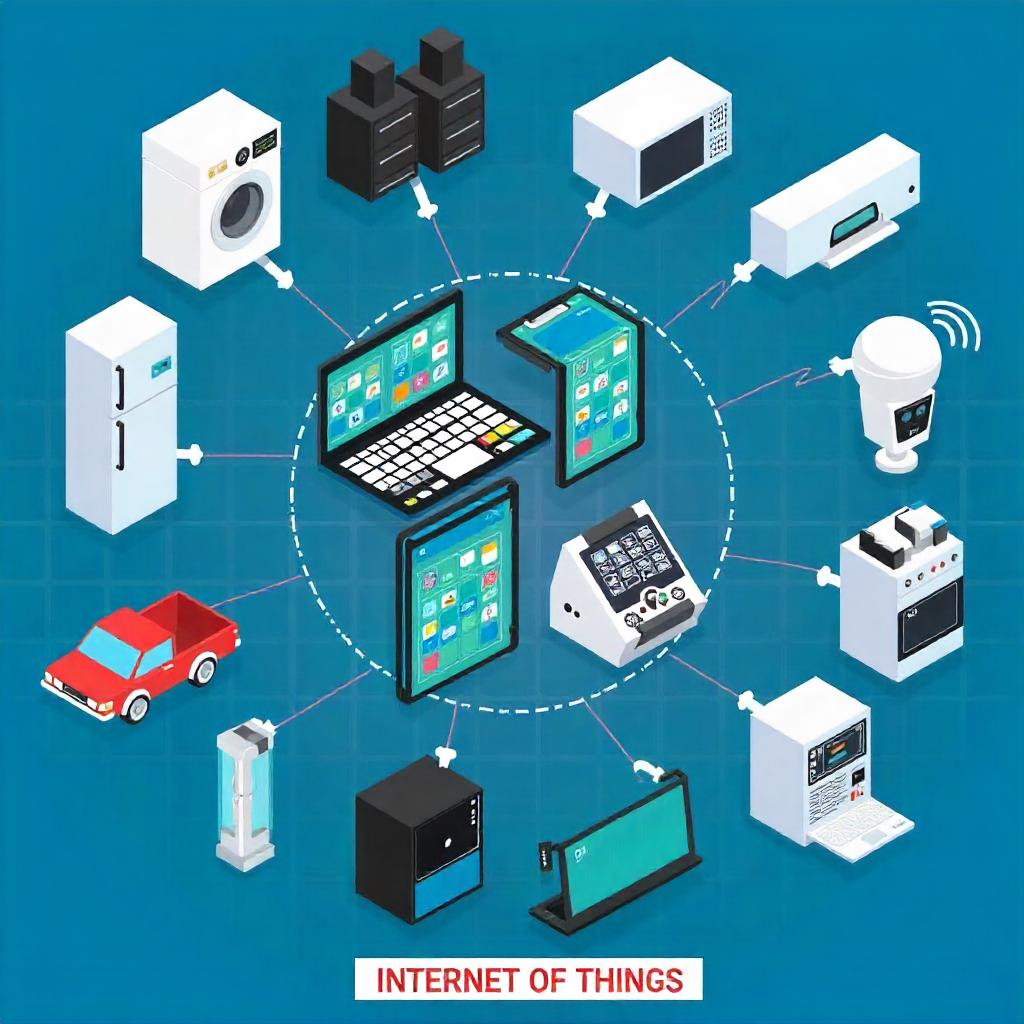
\includegraphics[width=0.45\textwidth]{./capitulo_02/figures/IoT_concept}
\caption{\textit{Internet de las Cosas} (crédito: Imagen por macrovector en \textit{Freepik}). \label{fig:IoTc}}
\end{center}
\end{minipage}
\end{figure}



\section{LoRA \textit{(Long Range)}}

\textit{\acrshort{lora-acronym}} es una tecnología de modulación de radiofrecuencia (\textit{\acrshort{rf}}) diseñada para redes de área amplia de baja potencia (\textit{\acrshort{lpwan-acronym}}). Derivada de la técnica \textit{\glspl{css} (\acrshort{css-acronym})}, codifica información en ondas de radio mediante chirridos, similar a la comunicación de delfines y murciélagos. Esta técnica permite comunicaciones de largo alcance, hasta tres millas (cinco kilómetros) en áreas urbanas y hasta 10 millas (15 kilómetros) o más en áreas rurales con línea de visión. \textit{\acrshort{lora-acronym}} proporciona comunicaciones de largo alcance con requisitos de energía ultrabajos, lo que permite que los dispositivos funcionen con baterías durante hasta 10 años \cite{Lora, doc_whatislorawan, doc_overviewsemtech}. Según Bertoleti \cite{bertoleti2019proyectos}, esta tecnología es ideal para aplicaciones (\textit{\acrshort{iot-acronym}}), dado que opera en bandas de frecuencia sin licencia y es resistente a interferencias.

\paragraph{Bandas de Frecuencia y Configuración Regional\\}
\textit{\acrshort{lora-acronym}} opera en bandas de frecuencia sub-gigahertz específicas para cada región para evitar interferencias. En América, \textit{\acrshort{lora-acronym}} utiliza la banda de 902-928 MHz; en Europa, 863-870 MHz; y en China, 779-787 MHz. Los planes de frecuencia específicos y parámetros de cada región están detallados en los documentos \cite{doc_frequencyplans, doc_regionalparameters}.

\paragraph{Ventajas y Limitaciones de \acrshort{lora-acronym}\\}
\textit{\acrshort{lora-acronym}} ofrece varias ventajas clave \cite{doc_overviewsemtech, doc_loraphysemtech}:
\begin{itemize}
    \item Alcance Extenso y Eficiencia Energética: \textit{\acrshort{lora-acronym}} permite la comunicación de datos a grandes distancias con bajo consumo de energía.
    \item Inmunidad a Interferencias: Al operar en bandas de baja frecuencia y utilizar \textit{\acrshort{css-acronym}}, \textit{\acrshort{lora-acronym}} minimiza la interferencia de otros dispositivos.
    \item Costo-Efectividad: Comparado con otras tecnologías, \textit{\acrshort{lora-acronym}} reduce los costos de infraestructura y mantenimiento.
\end{itemize}

Sin embargo, \textit{\acrshort{lora-acronym}} tiene limitaciones en la tasa de transmisión de datos, con un máximo de alrededor de 37.5 kbps, lo que la hace inadecuada para aplicaciones que requieren transmisión de grandes volúmenes de datos, como video. Además, \textit{\acrshort{lora-acronym}} no incorpora encriptación de datos en su capa física, por lo que los desarrolladores deben implementar medidas de seguridad en capas superiores \cite{doc_overviewsemtech}.


\section{\textit{LoRaWAN (Long Range Wide Area Network)}}

\textit{\acrshort{loraw}} es el protocolo de red que permite organizar y gestionar redes de dispositivos que utilizan \textit{\acrshort{lora-acronym}} como capa física. Este protocolo, administrado por la \textit{\acrshort{lora-acronym} Alliance}, es de código abierto y permite una estructura de red en la cual miles de dispositivos pueden conectarse y enviar datos a un servidor de red a través de \textit{gateways} (puntos de acceso). \textit{\acrshort{loraw}} facilita una comunicación bidireccional segura, escalable y de bajo consumo energético, adaptándose a los requerimientos de aplicaciones \textit{\acrshort{iot-acronym}} a gran escala \cite{doc_aboutlorawan, doc_lorawanstandardsemtech}. La Figura ~\ref{fig:loracapas} muestra la estructura de capas de \textit{\acrshort{lora-acronym}} y \textit{\acrshort{loraw}}, detallando las opciones \textit{\acrshort{mac-acronym}, \gls{mac} } y su integración con la capa física de \textit{\acrshort{lora-acronym}}.

\begin{figure}[H]
\leavevmode
\begin{minipage}{\textwidth}
\begin{center}
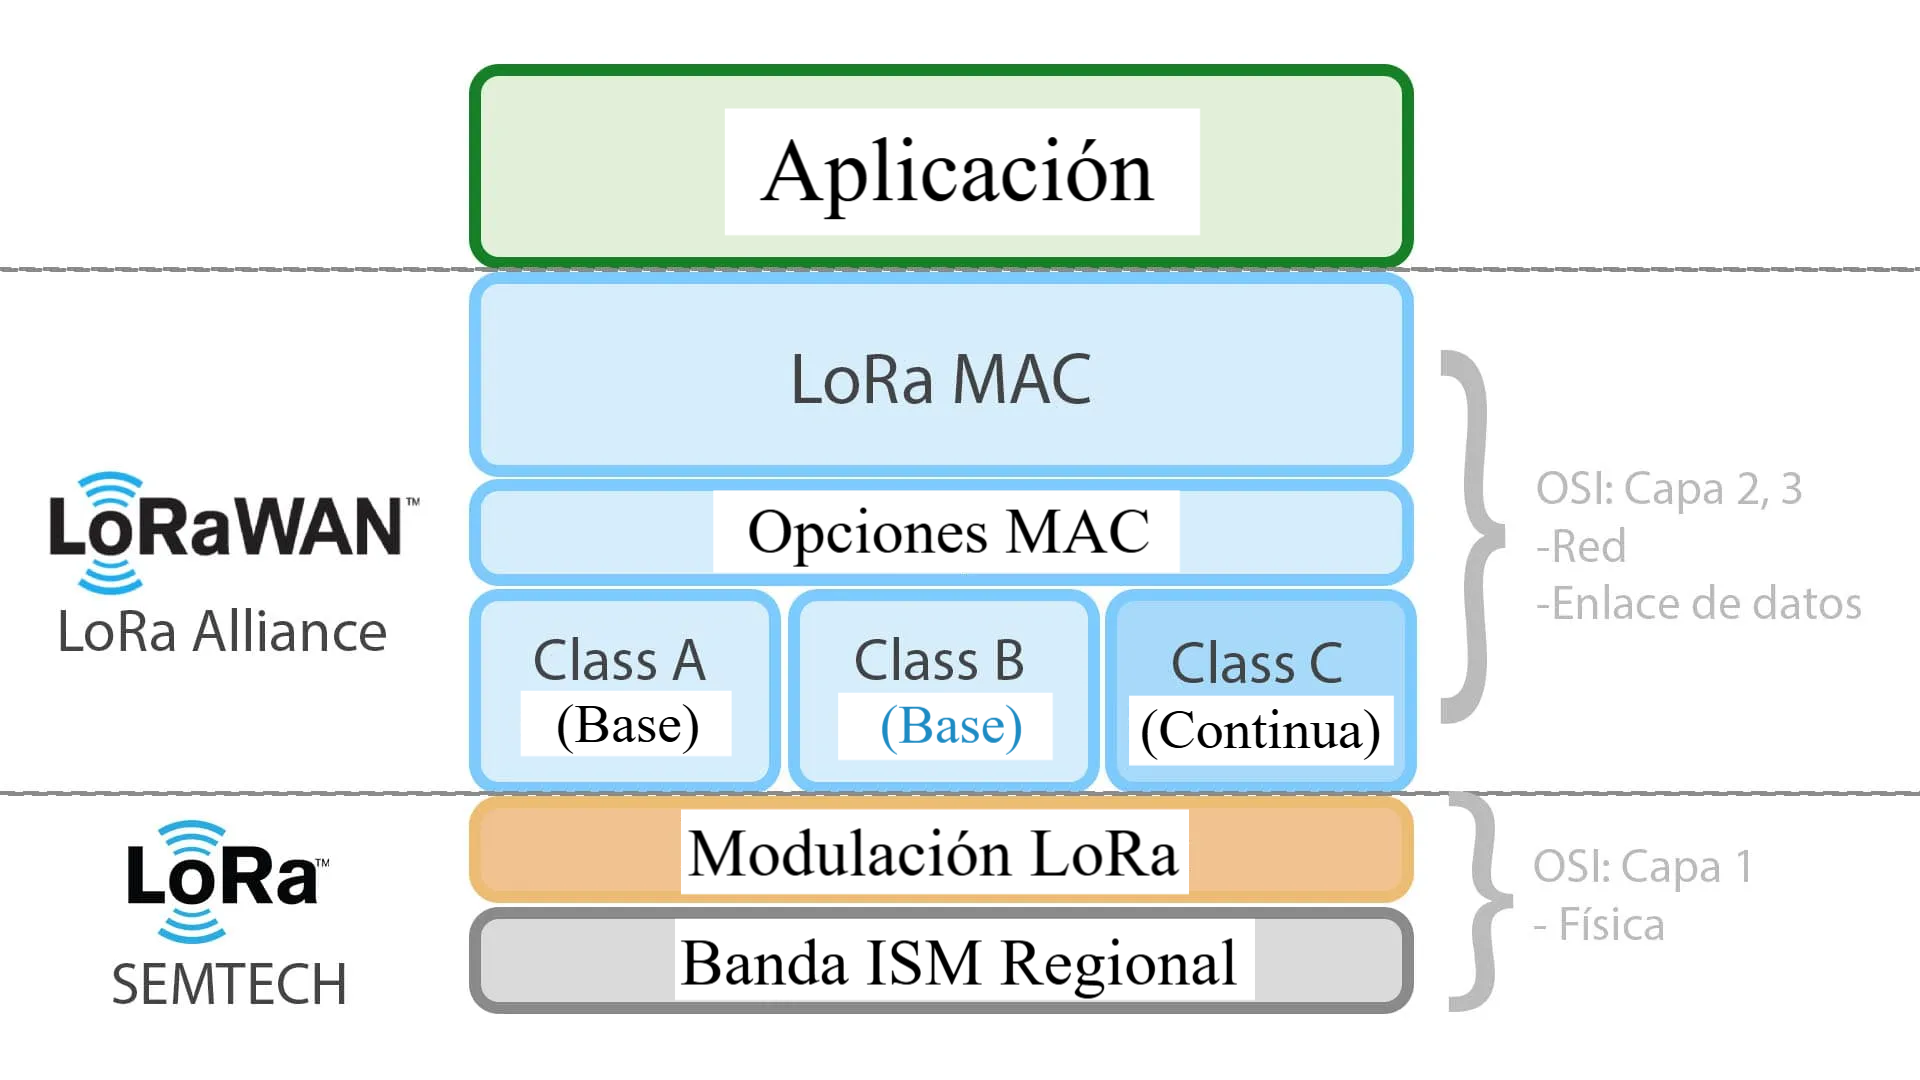
\includegraphics[scale=0.15]{./capitulo_02/figures/LoraLoraWAN.png}
\caption{Estructura de capas de \textit{\acrshort{lora-acronym}} y \textit{\acrshort{loraw}} \cite{doc_aboutlorawan}. \label{fig:loracapas}}
\end{center}
\end{minipage}
\end{figure}

\textit{\acrshort{lora-acronym}} se puede comparar con los cables físicos que interconectan los dispositivos en una red \textit{Ethernet}, mientras que \textit{\acrshort{loraw}} representa el protocolo de comunicación que gestiona el intercambio de datos entre los dispositivos, similar a cómo una red \textit{Ethernet} utiliza direcciones \textit{\acrshort{mac-acronym}} e \textit{IP} para coordinar la comunicación entre sus componentes.

\paragraph{Arquitectura de \acrshort{loraw}\\}
La arquitectura de \textit{\acrshort{loraw}} presenta una topología conocida como ``Estrella de Estrellas'' \textit{(Star of Stars)}, compuesta por cuatro elementos principales: dispositivos finales (nodos), \textit{gateways} (puertas de enlace), servidor de red y servidor de aplicación. Los dispositivos finales, generalmente constituidos por sensores o actuadores, utilizan la capa física \textit{\acrshort{lora-acronym}} para compartir información adquirida con el \textit{gateway}. El \textit{gateway}, a su vez, recibe esta información y la transmite al servidor de red mediante una comunicación \textit{\gls{backhaul-glossary}} (una red de retorno), que puede ser a través de redes \textit{Wi-Fi}, \textit{Ethernet} o redes móviles celulares \cite{sierra2023geolocalizacion}.\\

El servidor de red se encarga de recibir los paquetes de datos enviados por los nodos, decodificarlos y aplicar protocolos de seguridad, permitiendo que cada aplicación reciba los datos necesarios del servidor de red. Este protocolo facilita la recopilación de datos en un solo \textit{gateway} desde varios nodos ubicados a diferentes distancias, incluso kilómetros, a través de una comunicación unidireccional, aunque en algunos casos se utiliza la comunicación bidireccional entre nodo y \textit{gateway}. Finalmente, los datos se envían al servidor de aplicaciones, encargado de procesar la carga útil. Esta arquitectura permite administrar miles de dispositivos en una sola red, optimizando la escalabilidad y reduciendo los costos de infraestructura \cite{doc_whatislorawan, bertoleti2019proyectos}. En la Figura ~\ref{fig:arquitectura} se muestra la arquitectura de red previamente descrita.

\begin{figure}[H]
\leavevmode
\begin{minipage}{\textwidth}
\begin{center}
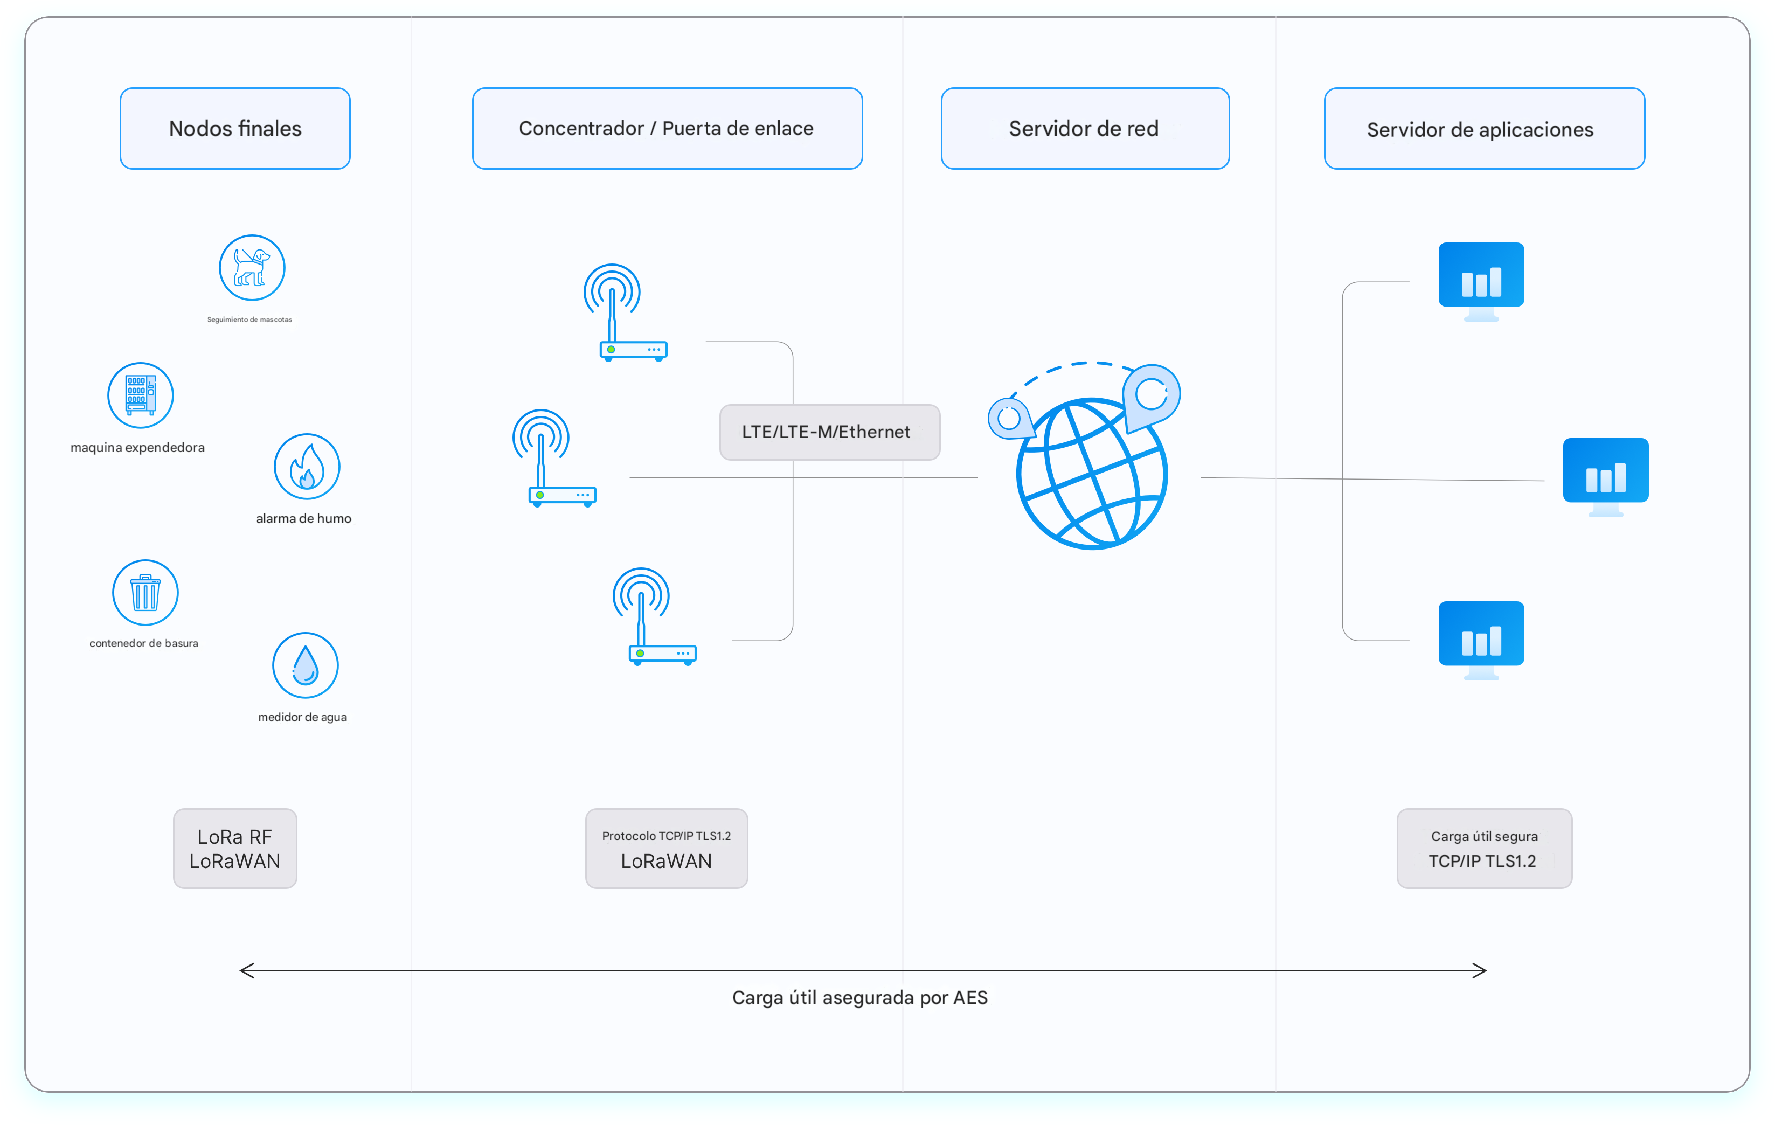
\includegraphics[scale=0.22]{./capitulo_02/figures/architecture.png}
\caption{Una arquitectura típica de red \textit{\acrshort{loraw}} \cite{Lora3}. \label{fig:arquitectura}}
\end{center}
\end{minipage}
\end{figure}

\paragraph{Clases de Dispositivos en \acrshort{loraw}\\}

\textit{\acrshort{loraw}} define tres clases de dispositivos, cada una optimizada para diferentes perfiles de uso y consumo energético \cite{doc_aboutlorawan, doc_lorawanstandardsemtech}:
\begin{itemize}
    \item \textbf{Clase A}: Dispositivos que solo reciben datos después de transmitir, ideal para sensores de bajo consumo.
    \item \textbf{Clase B}: Dispositivos con ventanas de recepción adicionales sincronizadas mediante balizas.
    \item \textbf{Clase C}: Dispositivos en escucha continua, adecuado para dispositivos conectados a una fuente de energía constante.
\end{itemize}

La Figura ~\ref{fig:loraclass} ilustra las características de cada clase de dispositivo en \textit{\acrshort{loraw}}, mostrando el momento de transmisión y las ventanas de recepción para cada clase. En la clase A, los dispositivos abren dos ventanas de recepción después de la transmisión, con retardo entre ellas, lo cual permite eficiencia energética. En la clase B, se añaden balizas de sincronización, lo que permite ventanas de recepción programadas en momentos específicos. La clase C, por otro lado, está en escucha continua, lo que minimiza la latencia de recepción de datos, pero aumenta el consumo de energía. Esta figura ayuda a visualizar las diferencias en el comportamiento de las tres clases y su adecuación para distintos tipos de aplicaciones.

\begin{figure}[H]
\leavevmode
\begin{minipage}{\textwidth}
\begin{center}
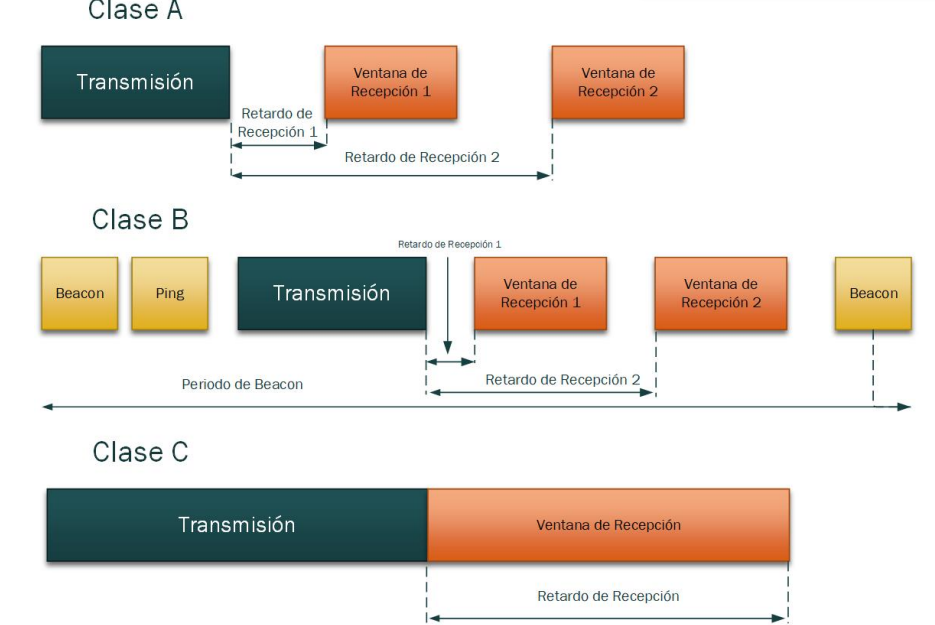
\includegraphics[scale=0.5]{./capitulo_02/figures/claseslora.png}
\caption{Clases de Dispositivos en \textit{\acrshort{loraw}} \cite{morales2021lorawan}. \label{fig:loraclass}}
\end{center}
\end{minipage}
\end{figure}

\paragraph{Seguridad en \acrshort{loraw}\\}
La seguridad es un componente esencial en \textit{\acrshort{loraw}}, diseñado para garantizar la autenticación, integridad y confidencialidad en las comunicaciones \textit{\acrshort{iot-acronym}}. \textit{\acrshort{loraw}} implementa una doble capa de protección con tres claves principales:
\begin{enumerate}
    \item \textbf{Autenticación en la Capa de Red}: La \gls{nwkskey-glossary} (\textit{nwkskey-acronym}) autentica cada dispositivo, asegurando que solo nodos autorizados puedan acceder a la red. También valida la integridad de cada mensaje mediante un código de integridad (\textit{MIC}) para prevenir alteraciones en los datos.
    \item \textbf{Encriptación en la Capa de Aplicación}: La \gls{appskey-glossary}, (\textit{\gls{appskey-acronym}}) cifra y descifra los datos transmitidos, asegurando que solo el dispositivo y el servidor de aplicación puedan acceder al contenido, lo cual protege la privacidad del usuario \cite{doc_overviewsemtech, doc_loraphysemtech, ttn_security}.
    \item \textbf{Clave de Aplicación (\textit{\acrshort{appkey-acronym}})}: En el proceso de activación, los dispositivos que utilizan activación por aire (\textit{\acrshort{otaa-acronym}}) generan las claves de sesión (\textit{\acrshort{nwkskey-acronym}} y \textit{\acrshort{appskey-acronym}}) a partir de una clave de aplicación única (\textit{\acrshort{appkey-acronym}}). Esto permite que las claves de sesión se regeneren en cada activación, añadiendo una capa adicional de seguridad dinámica \cite{ttn_security, lorawan_security_whitepaper}.
\end{enumerate}

Para prevenir ataques de repetición, \textit{\acrshort{loraw}} emplea contadores de tramas (\textit{frame counters}), evitando que los mensajes antiguos se retransmitan. Además, utiliza cifrado \textit{\gls{aes-acronym}},  (\textit{\gls{aes}}) en modo \textit{CTR} (\textit{Counter Mode}) para proteger los datos y \textit{\acrshort{cmac-acronym}} (\textit{\gls{cmac}}) para verificar la integridad, ambos métodos aprobados por el \textit{NIST} (\textit{National Institute of Standards and Technology}).

La Figura ~\ref{fig:seclora} ilustra este flujo de seguridad en \textit{\acrshort{loraw}}. En ella, cada dispositivo obtiene las claves de sesión \textit{\acrshort{nwkskey-acronym}} y \textit{\acrshort{appskey-acronym}} del \textit{Join Server} durante el proceso de activación. La \textit{\acrshort{nwkskey-acronym}} asegura la comunicación con el \textit{\acrshort{loraw} Network Server}, mientras que la \textit{\acrshort{appskey-acronym}} protege los datos entre el dispositivo y el \textit{Application Server}. Los \textit{gateways} actúan como intermediarios en este proceso, transmitiendo datos entre los dispositivos y el servidor de red, lo cual fortalece la seguridad de extremo a extremo en la red \textit{\acrshort{loraw}}.

\begin{figure}[H]
\leavevmode
\begin{minipage}{\textwidth}
\begin{center}
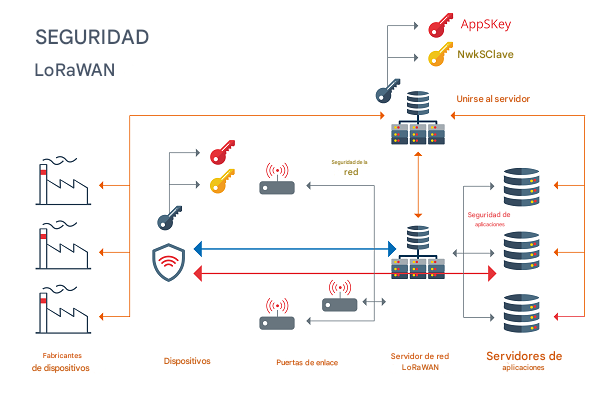
\includegraphics[scale=0.6]{./capitulo_02/figures/Lorasec.png}
\caption{Diagrama de Seguridad en \textit{\acrshort{loraw}} \cite{lorawan_security_whitepaper}. \label{fig:seclora}}
\end{center}
\end{minipage}
\end{figure}



\paragraph{Tasa de Datos Adaptativa (\gls{adr-glossary}) en \acrshort{loraw}\\}
\textit{\acrshort{loraw}} incorpora el mecanismo de (\gls{adr-acronym} que ajusta automáticamente el factor de dispersión, el ancho de banda y la potencia de transmisión según la distancia al \textit{gateway} y la calidad de la señal. Esto permite que dispositivos cercanos al \textit{gateway} usen menos potencia y una mayor tasa de datos, mientras que los dispositivos más alejados incrementan el factor de dispersión para mejorar la sensibilidad.


\paragraph{Parámetros Regionales y Configuración\\}
El protocolo \textit{\acrshort{loraw}} también permite adaptarse a normativas regionales específicas, detalladas en \cite{doc_regionalparameters}. Estas regulaciones incluyen los límites de potencia de transmisión y las bandas de frecuencia permitidas. \cite{doc_frequencyplans} es una referencia para comprender las configuraciones regionales. \\

\textit{\acrshort{lora-acronym}} y \textit{\acrshort{loraw}} constituyen una combinación robusta para aplicaciones de \textit{\acrshort{iot-acronym}} que requieren comunicación de largo alcance y bajo consumo. \textit{\acrshort{lora-acronym}} permite comunicación de largo alcance y eficiente en consumo, mientras que \textit{\acrshort{loraw}} estructura la red con seguridad, escalabilidad y gestión de dispositivos.


\section{\textit{Helium Networks}}

\textit{Helium} es una red global distribuida de puntos de acceso que crean cobertura inalámbrica pública de largo alcance para dispositivos \textit{\acrshort{iot-acronym}} y celulares habilitados para \textit{\acrshort{loraw}}. Los \textit{Hotspots \acrshort{loraw}™} (puntos calientes) producen y se compensan en \textit{\acrshort{iot-acronym}}, la criptomoneda nativa de la cadena de bloques \textit{Helium}. La cadena de bloques \textit{Helium} es una nueva cadena de bloques pública de código abierto creada enteramente para incentivar la creación de redes inalámbricas físicas y descentralizadas. Hoy en día, \textit{Helium IoT Network} y sus cientos de miles de \textit{Hotspots} brindan acceso a la red \textit{\acrshort{loraw}} más grande del mundo \cite{heliumDocs}.

\section{\textit{RFID}}

La identificación por radiofrecuencia, o \textit{\acrshort{rfid-acronym}}, es un término genérico para denominar a las tecnologías que utilizan ondas de radio. \textit{\acrshort{rfid-acronym}} es un método simple y automático de recolección de datos sobre un activo o producto (identificación, ubicación, estado, fecha y hora, etc.) de forma más rápida y fácil, sin requerir intervención humana y evitando errores.

Existen diversos métodos para realizar la identificación de objetos utilizando tecnología \textit{\acrshort{rfid-acronym}}, pero el más común consiste en almacenar un número de serie que identifica un producto (y posiblemente otro tipo de información adicional) en un microchip adjunto a una antena. El chip y la antena juntos conforman un \textit{Tag \acrshort{rfid-acronym}}. La antena permite al chip transmitir la información almacenada a un lector. Este lector convierte las ondas de radio de las etiquetas \textit{\acrshort{rfid-acronym}} en datos que pueden ser transmitidos a un sistema informático \cite{rfid}. En la Figura \ref{fig:RFID}, se ilustra la Interfaz Lector-Etiqueta y la Interfaz Lector-Sistema de un sistema \textit{\acrshort{rfid-acronym}}.

\begin{figure}[H]
\leavevmode
\begin{minipage}{\textwidth}
\begin{center}
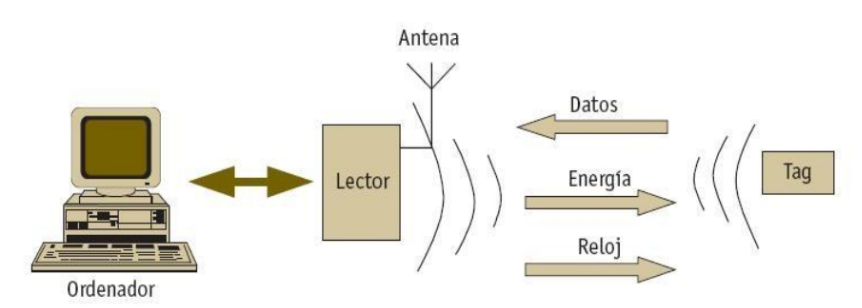
\includegraphics[scale=0.6]{./capitulo_02/figures/RFIDD}
\caption{Modelo de Sistema \textit{\acrshort{rfid-acronym}} \cite{proyectoRFID}. \label{fig:RFID}}
\end{center}
\end{minipage}
\end{figure}

\paragraph{Componentes Principales de un Sistema \textit{\acrshort{rfid-acronym}}\\}

Un sistema \textit{\acrshort{rfid-acronym}} consta de tres componentes esenciales:

\begin{enumerate}
    \item \textbf{Etiquetas \textit{\acrshort{rfid-acronym} (Tags):}}
    \begin{itemize}
        \item Contienen un microchip y una antena que permiten la transmisión de datos.
        \item Clasificación:
        \begin{itemize}
            \item \textit{Activas:} Equipadas con batería interna, permiten comunicación a distancias mayores.
            \item \textit{Pasivas:} Sin fuente de energía interna, se activan por el campo electromagnético del lector.
        \end{itemize}
        \item Almacenan información única que identifica el objeto al que están asociadas \cite{RFidtech}.
    \end{itemize}
    \item \textbf{Lector \textit{\acrshort{rfid-acronym} (Reader):}}
    \begin{itemize}
        \item Dispositivo que emite señales de radio para activar las etiquetas y leer los datos almacenados.
        \item Está compuesto por una antena y un procesador que interpreta la información transmitida por las etiquetas.
    \end{itemize}
    \item \textbf{Middleware y Sistema de Gestión:}
    \begin{itemize}
        \item Gestiona y procesa los datos recopilados por los lectores para integrarlos en sistemas de administración y monitoreo en tiempo real \cite{Mechanismiot}.
    \end{itemize}
\end{enumerate}

La Figura \ref{fig:RFIDCommunication} muestra el flujo interno de comunicación entre un lector \acrshort{rfid-acronym} y una etiqueta. Incluye los componentes claves.


\begin{figure}[H]
\leavevmode
\begin{minipage}{\textwidth}
\begin{center}
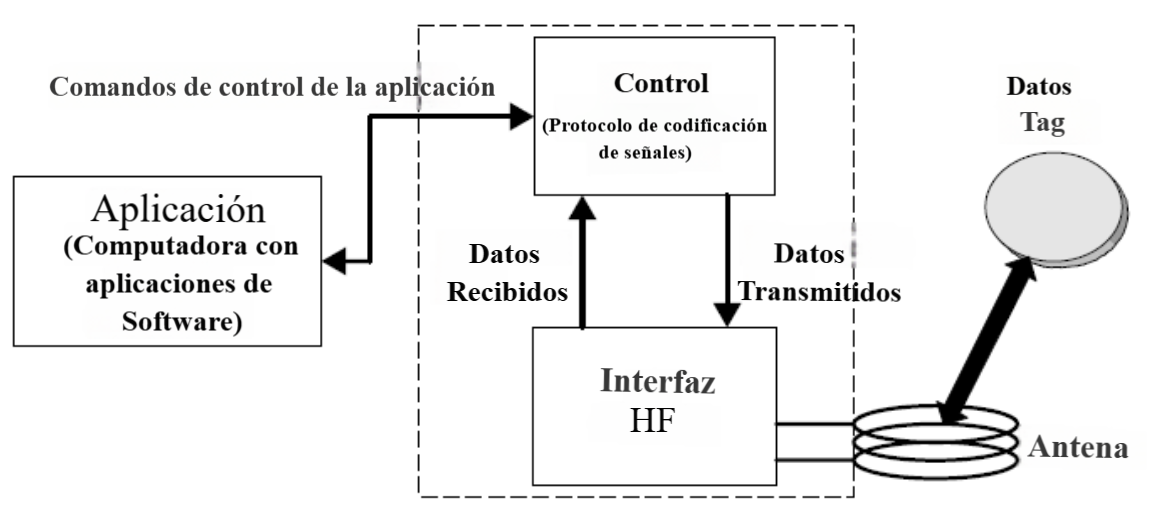
\includegraphics[scale=0.3]{./capitulo_02/figures/RFIDmodelsf.png}
\caption{Modelo de comunicación entre el lector y los tags en un sistema \textit{\acrshort{rfid-acronym}} \cite{RFidtech}. \label{fig:RFIDCommunication}}
\end{center}
\end{minipage}
\end{figure}


\paragraph{Funcionamiento de \textit{\acrshort{rfid-acronym}}\\}

El lector genera un campo electromagnético que activa las etiquetas pasivas, permitiendo la transferencia de datos a través de la modulación de ondas de radio. Los datos recibidos por el lector son procesados y enviados a un sistema de gestión. En el caso de etiquetas activas, estas utilizan su batería para transmitir información de forma autónoma, logrando mayores alcances \cite{8550722}.

En algunos sistemas \acrshort{rfid-acronym}, la comunicación entre los componentes se organiza siguiendo un modelo maestro-esclavo. En este modelo, los principales actores tienen roles claramente definidos:
\begin{itemize}
    \item Aplicación (maestro): Envía comandos al lector para iniciar la comunicación y recibe los datos procesados desde las etiquetas.
    \item Lector: Actúa como intermediario entre la aplicación y las etiquetas. Recibe los comandos de la aplicación, los traduce a señales de radio para las etiquetas, y devuelve las respuestas de las etiquetas a la aplicación.
    \item Tags (esclavas): Responden a las señales del lector, enviando la información almacenada en su memoria interna.
\end{itemize}

La Figura \ref{fig:MasterSlaveFlow} ilustra este flujo de datos, mostrando cómo las etiquetas y el lector interactúan bajo la dirección de la aplicación. Este modelo es común en aplicaciones que requieren un control jerárquico, como sistemas de control de acceso o gestión logística centralizada.

\begin{figure}[H]
\leavevmode
\begin{minipage}{\textwidth}
\begin{center}
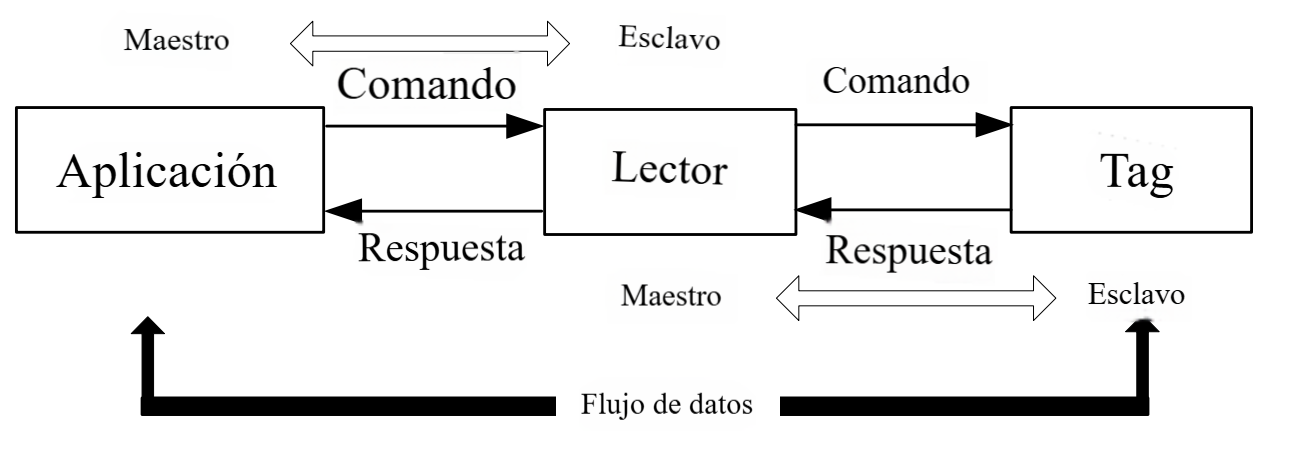
\includegraphics[scale=0.3]{./capitulo_02/figures/RFID_MSf.png}
\caption{Flujo de datos en un sistema \textit{\acrshort{rfid-acronym}} basado en el modelo maestro-esclavo \cite{Mechanismiot}. \label{fig:MasterSlaveFlow}}
\end{center}
\end{minipage}
\end{figure}

Sin embargo, no todos los sistemas \acrshort{rfid-acronym} utilizan este modelo. Algunos sistemas optan por arquitecturas diferentes, dependiendo de sus necesidades y del tipo de etiquetas empleadas:
\begin{itemize}
    \item Sistemas Autónomos (Peer-to-Peer): El lector opera de manera autónoma, identificando etiquetas dentro de su alcance sin necesidad de comandos desde una aplicación maestra. Este enfoque es común en sistemas de inventarios masivos.
    \item Tags Activas con Comunicación Directa: En redes \acrshort{rfid-acronym} activas, las etiquetas con batería interna pueden comunicarse directamente con un servidor o receptor, eliminando la necesidad de un lector intermediario. Este modelo es ideal para rastreo de activos o vehículos en grandes áreas.
    \item Sistemas Distribuidos o en Red: Varios lectores pueden operar como nodos independientes en una red, reportando datos directamente a un servidor central sin jerarquías estrictas.
\end{itemize}

Cada modelo tiene sus ventajas y limitaciones. Mientras que el modelo maestro-esclavo es efectivo para aplicaciones que requieren control centralizado, los sistemas autónomos o distribuidos son más adecuados para entornos flexibles y escalables. La elección del modelo dependerá del caso de uso específico, el tipo de etiquetas y la infraestructura disponible.

\paragraph{Características Clave de \textit{\acrshort{rfid-acronym}}\\}

\begin{itemize}
    \item \textbf{Identificación sin contacto:} No requiere línea de vista directa, a diferencia de los códigos de barras.
    \item \textbf{Capacidad de lectura simultánea:} Puede identificar múltiples etiquetas en una sola operación.
    \item \textbf{Variedad de frecuencias:}
    \begin{itemize}
        \item \textit{LF (Low Frequency):} 125-134 kHz, corto alcance (10 cm), ideal para control de acceso.
        \item \textit{HF (High Frequency):} 13.56 MHz, alcance de hasta 1 metro, común en tarjetas inteligentes.
        \item \textit{UHF (Ultra High Frequency):} 860-960 MHz, para logística e inventarios, con alcance de varios metros.
    \end{itemize}
    \item \textbf{Durabilidad:} Las etiquetas pasivas tienen una vida útil prolongada, ya que no requieren baterías.
    \item \textbf{Seguridad:} Implementa medidas de autenticación y encriptación para proteger los datos transmitidos \cite{RFidtech, Mechanismiot}.
\end{itemize}

\paragraph{Aplicaciones de \textit{\acrshort{rfid-acronym}}\\}

\begin{enumerate}
    \item \textbf{Logística y Gestión de Inventarios:}
    \begin{itemize}
        \item Seguimiento automatizado de productos y monitoreo en tiempo real en cadenas de suministro.
    \end{itemize}
    \item \textbf{Control de Acceso:}
    \begin{itemize}
        \item Uso en sistemas de seguridad para edificios y eventos.
    \end{itemize}
    \item \textbf{Salud y Farmacéutica:}
    \begin{itemize}
        \item Monitoreo de equipos médicos y rastreo de medicamentos para prevenir falsificaciones.
    \end{itemize}
    \item \textbf{\textit{\acrshort{iot-acronym}} y Ciudades Inteligentes:}
    \begin{itemize}
        \item Integración en soluciones inteligentes para rastreo y gestión en tiempo real \cite{Mechanismiot, 8550722}.
    \end{itemize}
\end{enumerate}

\textit{\acrshort{rfid-acronym}} es una tecnología versátil y eficiente, especialmente en combinación con \textit{\acrshort{iot-acronym}}. Su capacidad para identificar objetos de forma inalámbrica y sin contacto la convierte en una solución clave en sectores como logística, seguridad y salud. Al operar en diversas frecuencias y con opciones de configuración activa y pasiva, \textit{\acrshort{rfid-acronym}} se adapta a una amplia variedad de aplicaciones \cite{8550722, RFidtech}.

  

\section{Sistema de Geolocalización}

La geolocalización es el reconocimiento de la posición de un dispositivo en el espacio real. El  (\textit{\gls{gps-acronym}}, por sus siglas en inglés) es la forma más conocida para obtener la localización geográfica, ubicando el dispositivo con una precisión de unos pocos metros. Los datos obtenidos de la posición del \textit{\acrshort{gps-acronym}} no dependen exclusivamente de la conexión a la red de Internet, sino también de la geolocalización del dispositivo cuando no se encuentra fuera de la cobertura de los satélites geoestacionarios. Esta tecnología no es recomendable para uso en interiores como edificios, casas o lugares cerrados, ya que la cobertura de los satélites \textit{\acrshort{gps-acronym}} es nula \cite{fombona2017posibilidades, benavides2021implementacion}.

\section{Servicios de Entrega y Logística}

La Gestión de la Entrega de Servicios, también conocida como gestión de la prestación de servicios, es un área clave en las empresas orientadas a los servicios. Consiste en un conjunto de procesos y prácticas destinados a garantizar la entrega eficaz y de alta calidad de servicios a los clientes. El Gerente de Entrega de Servicios es el responsable encargado de supervisar y coordinar estas actividades. El papel principal de la Gestión de la Entrega de Servicios es asegurarse de que los servicios proporcionados cumplan con las expectativas de los clientes en cuanto a calidad, plazos y rendimiento. Esto implica una gestión proactiva de proyectos, recursos y relaciones con los clientes \cite{gestion}.














\section{Antecedentes}

\subsection{Lokalisering av sensorer med LoRaWAN på Kalmar Länssjukhus (Año 2021)}
\textbf{Desarrollado por:} Nathalie Wetterskog, Jeanette Marie Victoria Skeppeland Hole.

En \cite{SkepplandHole2021} se evaluó un sistema de posicionamiento basado en sensores conectados a \textit{\acrshort{loraw}} para localizar sillas de ruedas en el hospital de Kalmar. Este sistema ayudaría al personal del hospital a encontrar sillas de ruedas perdidas, mejorando la eficiencia operativa. La metodología empleada consistía en la instalación de sensores en las sillas de ruedas, que estaban conectados al sistema de rastreo \textit{Traxmate}, una plataforma \textit{\acrshort{iot-acronym}} diseñada para rastrear dispositivos mediante la recolección de datos de ubicación y la visualización en tiempo real \cite{SkepplandHole2021}. 

Los principales parámetros evaluados fueron: la precisión de la ubicación geográfica, la fuerza de la señal recibida (\textit{\acrshort{rssi-acronym}}) y la latencia de transmisión. La precisión de la ubicación se determinó mediante trilateración usando las direcciones \textit{\acrshort{mac-acronym}} de los puntos de acceso \textit{Wi-Fi} cercanos, lo que subraya la metodología empleada en \cite{SkepplandHole2021}. La latencia de transmisión se calculó como el tiempo de retraso entre la señal emitida por el sensor y su recepción por el sistema.

Los resultados mostraron que \textit{\acrshort{loraw}} es adecuado para su uso en el entorno hospitalario debido a su capacidad para operar tanto en interiores como en exteriores, aunque se encontraron deficiencias en la exactitud del sistema de posicionamiento \cite{SkepplandHole2021}. 

Es importante destacar que ambos trabajos utilizan la tecnología de \textit{\acrshort{loraw}} para la geolocalización, pero presentan diferencias significativas en su enfoque: este utiliza trilateración con puntos de acceso \textit{Wi-Fi} para determinar la ubicación, mientras que la propuesta actual se apoya en una combinación de \textit{\acrshort{rfid-acronym}} y \textit{\gls{gnss-acronym}} para mejorar la seguridad y la validación del propietario \cite{SkepplandHole2021}. Estas diferencias subrayan la versatilidad de las tecnologías de geolocalización en distintos contextos.

\subsection{LoRaWAN for tracking inland routes of plastic waste: Introducing the smart TRACKPLAST bottle (Año 2023)}
\textbf{Desarrollado por:} Stavros Ponis, George Plakas, Eleni Aretoulaki, Dimitra Tzanetou, Theodoros Nikolaos Maroutas.

En \cite{Ponis2023}, se desarrolló un sistema para rastrear el flujo de residuos plásticos desde tierra hasta el mar, utilizando la tecnología \textit{\acrshort{loraw}}. A través del desarrollo de una botella inteligente \textit{TRACKPLAST}, se buscó emular y seguir el comportamiento de los residuos plásticos en el medio ambiente.

El diseño y la fabricación de la botella inteligente implicó la integración de sensores \textit{\acrshort{iot-acronym}} en una botella de plástico comercial. Los sensores fueron integrados de manera que no afectaran la apariencia o el comportamiento de la botella en el ambiente. Para la comunicación de las botellas inteligentes, se desarrolló una red \textit{\acrshort{lora-acronym}} específica. Esta red incluyó la instalación de tres \textit{gateways} en la región de \textit{Attiki}, cerca de Atenas, que eran utilizados para la trilateración y el seguimiento preciso de las botellas \cite{Ponis2023}. Se realizaron pruebas de conectividad para asegurar el funcionamiento correcto de la red.

El proyecto destacó el uso de servicios de geolocalización de la plataforma \textit{\acrshort{lora-acronym} Cloud Geolocation}, una \textit{\acrshort{api-acronym}} que trabaja con un servidor de red, que recibe metadatos como \textit{\acrshort{rssi-acronym}}, \textit{SNR} (\textit{Signal-to-Noise Ratio}) y \textit{\acrshort{toa-acronym}} (\textit{\gls{toa-glossary}}) de los \textit{gateways} para calcular las posiciones de los dispositivos. La geolocalización se logró específicamente mediante la técnica \textit{TDOA, \gls{tdoa}}. Además, se creó una plataforma en la nube para procesar y visualizar los datos recolectados por los sensores. La plataforma recibía las señales a través de los \textit{gateways}, analizaba los datos geoespaciales y los mostraba en un mapa, permitiendo a las autoridades locales rastrear las rutas de las botellas. Esta plataforma fue probada por expertos y usuarios finales para garantizar su funcionalidad y facilidad de uso \cite{Ponis2023}.

La validación del sistema se realizó en condiciones reales mediante una implementación piloto en la isla de \textit{Syros}, Grecia. Se desplegaron 69 botellas inteligentes y se siguieron sus movimientos en tiempo real desde abril hasta junio de 2022. Esta fase permitió obtener datos valiosos sobre el comportamiento y destino de los residuos plásticos.

Los resultados del proyecto fueron positivos. Las botellas \textit{TRACKPLAST} se rastrearon con éxito durante toda su vida útil de batería, proporcionando información crucial para la gestión de residuos plásticos. Los datos obtenidos ayudaron a las autoridades locales a comprender mejor los flujos de residuos plásticos y a implementar medidas preventivas para reducir la contaminación marina \cite{Ponis2023}.

Aunque ambos trabajos utilizan la tecnología de \textit{\acrshort{loraw}}, se enfocan en aplicaciones diferentes: el sistema de \textit{TRACKPLAST} se centra en el rastreo y análisis del comportamiento de los residuos plásticos, mientras que el presente trabajo busca fortalecer la seguridad del propietario a través de una integración de \textit{\acrshort{rfid-acronym}} y \textit{\acrshort{gnss-acronym}}. Esto demuestra la adaptabilidad de la tecnología de geolocalización para abordar problemáticas variadas y resaltar su potencial en distintos ámbitos.


\subsection{Smart Security System for Two-Wheelers (Año 2020)}
\textbf{Desarrollado por:} Niyati Rana, Pravesh Khatta, Antim Dev Mishra.

En \cite{Rana}, se desarrolló un sistema de seguridad para motocicletas y \textit{scooters} utilizando la tecnología \textit{\acrshort{iot-acronym}}. Este sistema incluye la creación de un prototipo que integra \textit{hardware} y \textit{software} para ofrecer protección contra robos. El sistema se construyó alrededor de la plataforma \textit{Arduino Mega} y emplea varios componentes clave: un sensor de huellas dactilares, un módulo \textit{GPS Neo-6M}, un módulo \textit{\acrshort{gsm-acronym}} y una alarma sonora.

El sensor de huellas dactilares se utiliza para autenticar al usuario antes de permitir el arranque del vehículo. Solo se puede arrancar el vehículo si la huella coincide con la registrada en el sistema. El módulo \textit{\acrshort{gsm-acronym}} se encarga de la comunicación entre el vehículo y el propietario, enviando mensajes \textit{\acrshort{sms-acronym}} en caso de detección de actividad sospechosa. El módulo \textit{\acrshort{gsm-acronym}} está conectado a la red móvil y vinculado al sistema de \textit{Arduino}. Si el sistema detecta un intento de manipulación no autorizado, el módulo \textit{\acrshort{gsm-acronym}} envía un mensaje de alerta al teléfono del propietario, quien recibe la notificación indicando el posible intento de robo. 

El sistema permite al propietario controlar ciertas funciones de forma remota mediante comandos \textit{\acrshort{sms-acronym}}. El propietario puede enviar un comando \textit{\acrshort{sms-acronym}} específico al módulo \textit{\acrshort{gsm-acronym}}, que lo transmite a la placa \textit{Arduino}, y esta ejecuta los comandos. Además, el sistema activa la alarma sonora para disuadir a los ladrones. Si el sensor de huellas detecta un intento de arranque no autorizado, se activa una alarma sonora, alertando a las personas cercanas y posiblemente ahuyentando al ladrón. Adicionalmente, se acciona el módulo \textit{\acrshort{gps-acronym}}, lo cual proporciona la ubicación del vehículo en tiempo real. Esto permite al propietario y a las autoridades localizar y recuperar el vehículo de manera más eficiente \cite{Rana}.

El proyecto logró desarrollar un prototipo funcional que proporciona una solución de seguridad eficaz y económica para vehículos de dos ruedas. Se logró un monitoreo en tiempo real, alertas inmediatas de intentos de robo, control remoto de funciones y disuasión mediante una alarma sonora, demostrando cómo la integración de tecnologías \textit{\acrshort{iot-acronym}} puede mejorar significativamente la seguridad de motocicletas y \textit{scooters} \cite{Rana}.

Es importante resaltar que, aunque este sistema de seguridad se centra en la protección de motocicletas y utiliza tecnologías como huellas dactilares y \textit{\acrshort{gsm-acronym}}, la propuesta actual se distingue al incorporar diferentes tecnologías, como \textit{\acrshort{rfid-acronym}} y geolocalización mediante \textit{\acrshort{loraw}}. Estas tecnologías adicionales buscan ofrecer un enfoque complementario en la validación de la identidad del usuario y el rastreo de la ubicación del vehículo, destacando la diversidad de soluciones tecnológicas aplicables en el ámbito de la seguridad vehicular.

\subsection{Smart Security System for Vehicles using Internet of Things (IoT) (Año 2018)}
\textbf{Desarrollado por:} Mithileysh Sathiyanarayanan, Santosh Mahendra, Rajesh Babu Vasu.

En \cite{Sathiyanarayanan2018}, se describe el desarrollo de un sistema de seguridad inteligente para vehículos utilizando la tecnología \textit{\acrshort{iot-acronym}}. El objetivo principal es transformar los sistemas de seguridad vehicular convencionales (\textit{CVSS}) en sistemas de seguridad vehicular inteligentes (\textit{SVSS}) que permitan el acceso y control remoto de los vehículos mediante un teléfono inteligente.

El sistema se construyó alrededor de varios componentes clave. Primero, un subsistema de identificación que emplea etiquetas \textit{\acrshort{rfid-acronym}} y un lector conectado a un microcontrolador \textit{Arduino Uno R3}. Cuando se intenta encender el vehículo, el sistema debe validar la etiqueta para permitir el arranque del motor. Otro subsistema de detección utiliza un receptor \textit{\acrshort{gps-acronym}} para obtener la ubicación en tiempo real del vehículo. Estos datos se envían al microcontrolador y se pueden ver en la aplicación móvil del propietario.

Para la salida y alerta, el sistema cuenta con indicadores \textit{LED}, un \textit{buzzer} y una pantalla \textit{LCD}. Si se detecta un intento de robo, el \textit{buzzer} emite una alarma sonora y los relés controlan el encendido del motor, bloqueando el arranque si no se autentica correctamente. Por último, el subsistema de control es manejado por el microcontrolador, que ejecuta comandos y procesa datos. Un módulo \textit{\acrshort{gsm-acronym}} conectado envía y recibe mensajes \textit{\acrshort{sms-acronym}}. Ante actividades sospechosas, el módulo envía alertas al propietario, quien puede bloquear el motor, activar la alarma o solicitar la ubicación del vehículo mediante comandos \textit{\acrshort{sms-acronym}}.

Además, cuenta con una aplicación móvil que permite al propietario ver la ubicación del vehículo, bloquear o desbloquear el motor y activar la alarma. También recibe alertas en tiempo real sobre intentos de robo y otras actividades de seguridad \cite{Sathiyanarayanan2018}.

Las pruebas del sistema se realizaron en varias etapas para asegurar su funcionalidad y efectividad. Estas pruebas demostraron que el sistema puede identificar al propietario de manera precisa mediante \textit{\acrshort{rfid-acronym}}, proporcionar la ubicación exacta del vehículo en tiempo real y enviar alertas instantáneas en caso de intento de robo. Además, la capacidad de control remoto a través de la aplicación móvil y comandos \textit{\acrshort{sms-acronym}} añadió una capa adicional de seguridad y conveniencia.

El proyecto logró desarrollar un sistema de seguridad vehicular inteligente que utiliza tecnologías \textit{\acrshort{iot-acronym}} para mejorar la protección y el control de vehículos. Este sistema ofrece una solución efectiva y económica para prevenir robos, con la ventaja adicional de proporcionar control remoto y monitoreo en tiempo real a través de teléfonos inteligentes \cite{Sathiyanarayanan2018}.

Este enfoque de seguridad vehicular, que combina tecnologías de \textit{\acrshort{iot-acronym}}, presenta características específicas que mejoran la protección de vehículos. Por otro lado, el trabajo actual utiliza tecnologías distintas, como una combinación de \textit{\acrshort{rfid-acronym}} y \textit{\acrshort{gnss-acronym}}, lo que permite un enfoque diferente en la validación y el rastreo, mostrando así la diversidad de aplicaciones en la seguridad de vehículos y la versatilidad de las tecnologías disponibles.


\subsection{Development of an IoT-Based (LoRaWAN) Tractor Tracking System (2022)}
\textbf{Desarrollado por:} Çağdaş Civelek.

En \cite{Civelek}, se describe el desarrollo de un sistema \textit{\acrshort{iot-acronym}} de rastreo para tractores utilizando \textit{\acrshort{loraw}}, con el objetivo de apoyar la agricultura de precisión en Turquía. Este proyecto surge ante la dificultad de implementar tecnologías avanzadas de monitoreo en áreas rurales, donde la infraestructura y los altos costos de soluciones comerciales basadas en \textit{\acrshort{lte-acronym}} limitan su adopción, especialmente para agricultores de pequeñas explotaciones. La solución busca proporcionar una herramienta asequible y de bajo consumo energético que permita monitorear en tiempo real la ubicación y el rendimiento de los tractores, optimizando así las operaciones agrícolas y el uso de recursos.

El sistema está construido en torno a un microcontrolador \textit{PIC18F46K22}, al cual se le acopla un módulo \textit{\acrshort{lora-acronym} RN2483} para la transmisión de datos en la banda de frecuencia \textit{\acrshort{ism-acronym}, \gls{ism-glossary}}. Esto permite la transmisión de datos a largas distancias sin necesidad de infraestructura de comunicación convencional. Además, el sistema integra un módulo \textit{GPS SE868K7-A}, que proporciona coordenadas precisas de la ubicación del tractor, y diversos sensores, incluidos un medidor de flujo de combustible y un sensor de torque en la toma de fuerza (\textit{PTO}), para obtener información detallada sobre el consumo de combustible y la eficiencia operativa del vehículo. La transmisión de los datos recolectados se realiza mediante un \textit{gateway \acrshort{loraw} Kerlink Wirnet}, que envía la información a un servidor en la nube. Allí, los datos se almacenan en una base de datos \textit{MySQL} y se muestran en tiempo real a través de una interfaz web, accesible desde dispositivos móviles o computadoras, permitiendo a los usuarios visualizar la posición del tractor y otras métricas de rendimiento relevantes para la gestión agrícola.

Durante las pruebas de campo realizadas en áreas rurales cercanas a la Universidad de Çukurova, el sistema mostró un rendimiento satisfactorio, logrando transmitir datos de forma confiable hasta 15 km en zonas con baja interferencia. La precisión del \textit{\acrshort{gps-acronym}}, con un margen de error de aproximadamente 3 metros, resultó adecuada para el monitoreo en entornos de cultivo, proporcionando una visión precisa de la ubicación y movimientos del tractor en el campo. Además, se destacó que el costo de producción del sistema ronda los \$55, significativamente menor que los \$795 que suelen costar las soluciones comerciales basadas en \textit{\acrshort{lte-acronym}}. Este bajo costo convierte al sistema en una alternativa viable y accesible para los agricultores que desean implementar tecnologías de monitoreo sin incurrir en elevados gastos.

Este trabajo demuestra cómo \textit{\acrshort{loraw}} puede adaptarse a las necesidades de la agricultura de precisión, permitiendo el rastreo y la gestión de maquinaria agrícola de manera rentable. Comparado con el enfoque de seguridad vehicular del presente trabajo, que emplea \textit{\acrshort{loraw}} en combinación con \textit{\acrshort{rfid-acronym}} y \textit{\acrshort{gnss-acronym}} para la autenticación y monitoreo, este sistema agrícola se enfoca en mejorar la eficiencia y sostenibilidad de la producción agrícola. Sin embargo, ambos estudios destacan la flexibilidad y efectividad de \textit{\acrshort{loraw}} en aplicaciones de \textit{\acrshort{iot-acronym}} para distintos contextos, mostrando su potencial para transformar tanto la agricultura como otros sectores que requieren soluciones de monitoreo remoto.

\subsection{Use of RFID Technology as a Reporting Mechanism in Vehicle Tracking System (2016)}
\textbf{Desarrollado por:} Mamudu Hamidu.

En \cite{Hamidu}, se describe un sistema de seguridad vehicular denominado \textit{Transport Highway Integrated Security System} (\textit{THISS}), diseñado para facilitar el rastreo en tiempo real y la notificación de incidentes en autopistas mediante tecnología \textit{\acrshort{rfid-acronym}}, \textit{\acrshort{gps-acronym}} y \textit{\acrshort{gsm-acronym}}. La motivación para este desarrollo surge de la necesidad de contar con una herramienta rápida y precisa que permita a los conductores reportar eventos críticos, como robos, accidentes o fallos mecánicos, y mejorar la seguridad en las carreteras, especialmente en situaciones donde la asistencia inmediata puede ser crucial.

El sistema utiliza un módulo \textit{\acrshort{rfid-acronym}} para activar la señal de emergencia de manera sencilla y rápida, junto con un \textit{\acrshort{gps-acronym}} que obtiene la ubicación exacta del vehículo. Una vez que el conductor activa el sistema mediante el escaneo de una tarjeta \textit{\acrshort{rfid-acronym}}, el \textit{\acrshort{gps-acronym}} comienza a recopilar las coordenadas, y el módulo \textit{\acrshort{gsm-acronym}} envía esta información a una base de datos central en tiempo real. Este proceso permite registrar y monitorear la ubicación del vehículo y clasificar el tipo de emergencia según el incidente reportado. Para su implementación, el sistema cuenta con una estructura de comunicación en la cual los datos de ubicación y emergencia se gestionan a través de la red \textit{\acrshort{gsm-acronym}/GPRS}, garantizando una cobertura amplia y una transmisión de datos confiable.

Los resultados obtenidos en las pruebas iniciales del sistema revelaron una alta efectividad en la notificación de incidentes y en el envío de la ubicación en tiempo real. Las alertas generadas contenían coordenadas precisas y se transmitieron de forma consistente, asegurando que los datos llegaran a la base de datos central sin demoras significativas. Este flujo continuo de información permite a las autoridades responder con mayor rapidez y precisión a los eventos reportados, reduciendo el tiempo de reacción en caso de emergencias. La infraestructura de comunicación mediante \textit{\acrshort{gsm-acronym}} también facilitó la recolección de datos de ubicación, consolidándolos en una base de datos para su análisis y monitoreo a largo plazo.

Este proyecto demuestra cómo el uso de \textit{\acrshort{rfid-acronym}}, \textit{\acrshort{gps-acronym}} y \textit{\acrshort{gsm-acronym}} en conjunto puede crear una solución de seguridad vehicular robusta y accesible, que ofrece una alternativa práctica para la gestión de emergencias en autopistas. A diferencia del presente trabajo, que emplea \textit{\acrshort{loraw}} y \textit{\acrshort{rfid-acronym}} en combinación con \textit{\acrshort{gnss-acronym}} para la autenticación y rastreo vehicular, el sistema \textit{THISS} se enfoca en la notificación rápida de eventos y la asistencia en carretera. Ambos sistemas destacan el valor de integrar diferentes tecnologías de comunicación y localización para mejorar la seguridad y la capacidad de respuesta en distintos escenarios de uso.

\fancyhead{}
\fancyfoot{}
\pagestyle{plain}

\lhead{Tecnologías utilizadas}

\chapter{Tecnologías utilizadas}

En este capítulo se presentan las herramientas utilizadas para el desarrollo de este trabajo. En primer lugar, para asegurar que las herramientas seleccionadas sean adecuadas, se realiza una comparación entre alternativas considerando los factores y características más importantes dentro de las actividades.

\section{Componentes de \textit{Hardware}}

Los componentes de hardware abarcan los dispositivos físicos necesarios para la ejecución del sistema, incluyendo microcontroladores, sensores y módulos de comunicación, que se encargan de realizar las tareas físicas y electrónicas requeridas.

\subsection{Placa de Desarrollo WiFi LoRa 32 (V3)}

La \textit{WiFi LoRa 32 (V3)} (véase Figura \ref{fig:heltec}) es una placa de desarrollo \textit{\acrshort{iot-acronym}} basada en el microcontrolador \textit{ESP32-S3FN8}, un procesador de doble núcleo de 32 bits que opera a una frecuencia de hasta 240 MHz. Esta placa está diseñada para aplicaciones de bajo consumo y alto rendimiento en redes inalámbricas, tales como ciudades inteligentes, sistemas de seguridad, agricultura conectada y control industrial. Una de las características principales es la integración de múltiples tecnologías de comunicación, incluyendo \textit{Wi-Fi}, \textit{\gls{ble-glossary} (\acrshort{ble-acronym})} y \textit{\acrshort{lora-acronym}}, lo que le permite ser utilizada en una variedad de entornos \cite{WiFiLoRa32V3}.

La placa cuenta con un transceptor de radio \textit{SX1262}, que permite la transmisión de datos en redes de largo alcance. Soporta modulaciones \textit{\acrshort{lora-acronym}} y \textit{FHSS} para aplicaciones de redes de baja potencia y larga distancia (\textit{LPWAN}), además de la modulación \textit{(G)FSK} para aplicaciones más tradicionales. Este transceptor cubre un rango de frecuencias de 150 MHz a 960 MHz, permitiendo el uso en bandas \textit{ISM} globales. El \textit{SX1262} está diseñado para cumplir con los requisitos de la capa física de la especificación \textit{\acrshort{loraw}} y se ajusta a las regulaciones internacionales de transmisión de radiofrecuencia, lo que lo hace adecuado para su implementación en diversas regiones del mundo \cite{SX1262}.

\begin{figure}[H]
\leavevmode
\begin{minipage}{\textwidth}
\begin{center}
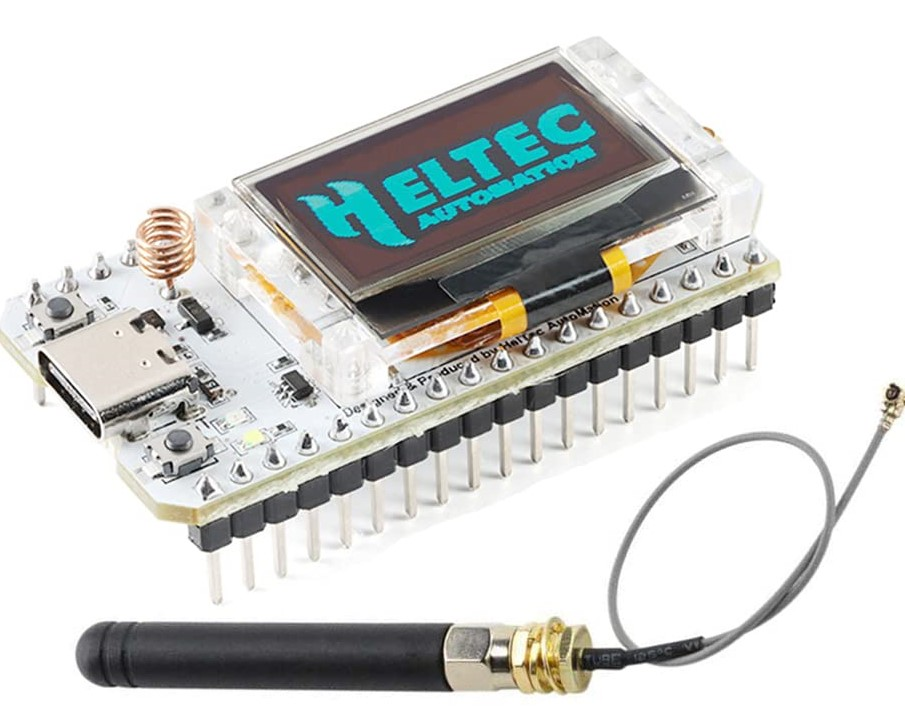
\includegraphics[scale=0.25]{./capitulo_03/figures/HW/Heltec.jpg}
\caption{Placa de desarrollo Heltec\label{fig:heltec}}
\end{center}
\end{minipage}
\end{figure}

La selección de la placa \textit{WiFi LoRa 32 (V3)} para esta investigación se basa en un análisis de diversas placas de desarrollo y herramientas de hardware, con el objetivo de identificar las tecnologías más adecuadas para aplicaciones de \textit{(\acrshort{iot-acronym})}. Se revisaron microcontroladores y transceptores \textit{\acrshort{lora-acronym}}, considerando su funcionalidad y rendimiento.

Según \cite{Cherkaoui2021Review}, los microcontroladores son componentes centrales en la transición de los sistemas embebidos hacia el \textit{\acrshort{iot-acronym}}. Estos dispositivos permiten manejar múltiples procesos de forma autónoma, lo que es esencial para la conectividad y automatización de dispositivos.

Las placas de desarrollo deben cumplir ciertos requisitos fundamentales, como conectividad y compatibilidad con diversas plataformas. En este contexto, se comparan las características clave de tres placas populares: el \textit{Wio E5 Mini}, el \textit{ESP32 Heltec LoRa WiFi V3} y el \textit{NÚCLEO-WL55JC}. Estas placas son reconocidas por su versatilidad y eficiencia en monitoreo y comunicación, como se documenta en diversos estudios \cite{Latifov2023Design, Jengsriwong2023LoRaWAN}.

Con el fin de seleccionar la placa de desarrollo, se establecieron una serie de criterios clave de evaluación que permiten analizar y comparar las opciones disponibles.

\begin{itemize}
    \item \textbf{Conectividad:} Se refiere a la capacidad del dispositivo para soportar diferentes tipos de comunicación y protocolos.
    \item \textbf{Frecuencia \acrshort{lora-acronym}:} Considera la compatibilidad del dispositivo con la frecuencia operativa del protocolo \textit{\acrshort{lora-acronym}} para esta región.
    \item \textbf{Características adicionales:} Incluye funcionalidades extra que pueden mejorar el rendimiento o la versatilidad del dispositivo, como sensores o interfaces de comunicación.
    \item \textbf{Compatibilidad con consolas:} Evalúa qué tan bien la placa puede integrarse con las plataformas de administración y control de dispositivos \textit{\acrshort{loraw}} que permiten la gestión y supervisión del dispositivo.
    \item \textbf{Tamaño/Dimensiones:} Este criterio evalúa la adecuación del tamaño del dispositivo ya que se requiere un diseño compacto.
    \item \textbf{Entornos de desarrollo (Facilidad):} Considera la facilidad de uso del entorno de desarrollo, lo que puede afectar la curva de aprendizaje y el tiempo de implementación.
\end{itemize}

Para reflejar el desempeño relativo de cada dispositivo, se empleó una escala del 1 al 3:

\begin{itemize}
    \item \textbf{3:} Indica el mejor rendimiento o la opción más favorable en ese criterio.
    \item \textbf{2:} Representa un rendimiento intermedio, adecuado pero no el mejor.
    \item \textbf{1:} Refleja un rendimiento limitado en comparación con los otros dispositivos.
\end{itemize}
A continuación, se presenta la tabla \ref{fig:Elec_Mic} comparativa que resume las características técnicas más relevantes de cada dispositivo, facilitando así la selección de la opción más adecuada para este proyecto.

\begin{table}[H]
\centering
\renewcommand{\arraystretch}{1.2} % Ajustar el espacio entre filas
\caption{Tabla comparativa entre Placas de Desarrollo}
\label{fig:Elec_Mic}
\begin{tabular}{|p{4.5cm}|p{1.8cm}|p{3cm}|p{2.6cm}|}
\hline
\textbf{Criterio/Placa}        & \textbf{Wio E5 Mini} & \textbf{ESP32 Heltec WiFi LoRa V3} & \textbf{NÚCLEO-WL55JC} \\ \hline
Conectividad                  &                 2                    & 3                                  & 2                      \\ \hline
Frecuencia LoRa               & 2                    & 3                                  & 3                      \\ \hline
Características adicionales   & 1                    & 3                                  & 1                      \\ \hline
Compatibilidad con consolas   & 3                    & 3                                  & 3                      \\ \hline
Tamaño/Dimensiones            & 3                    & 2                                  & 2                      \\ \hline
Entornos de desarrollo (Facilidad) & 2              & 2                                  & 1                      \\ \hline
\textbf{Total}                & \textbf{13}          & \textbf{16}                        & \textbf{12}            \\ \hline
\end{tabular}
\end{table}


De la tabla comparativa se determina que el \textit{WiFi LoRa V3} es el dispositivo más adecuado para la investigación. Este dispositivo fue seleccionado para las pruebas debido a su equilibrio entre conectividad y compatibilidad con diversos entornos de desarrollo, lo que lo convierte en una opción ideal para la fase de prototipado.


\subsection{Lector RFID MFRC522}

El \textit{MFRC522} (ver Figura \ref{fig:rc522rf}) es un circuito integrado de alto rendimiento diseñado para la lectura y escritura de tarjetas de identificación por radiofrecuencia (\textit{\acrshort{rfid-acronym}}) a 13.56 MHz, compatible con los estándares ISO/IEC 14443 A y tecnologías \textit{MIFARE} y \textit{NTAG}. Este módulo es ideal para aplicaciones de control de acceso, sistemas de pago sin contacto, y sistemas de seguimiento por identificación de objetos, brindando un diseño compacto y eficiente.

El \textit{MFRC522} está equipado con un transmisor integrado que permite la comunicación con tarjetas \textit{\acrshort{rfid-acronym}} sin necesidad de circuitos adicionales, proporcionando una distancia de operación de hasta 50 mm (dependiendo del diseño y tamaño de la antena) \cite{MFRC522Datasheet}. 

\begin{figure}[H]
\leavevmode
\begin{minipage}{\textwidth}
\begin{center}
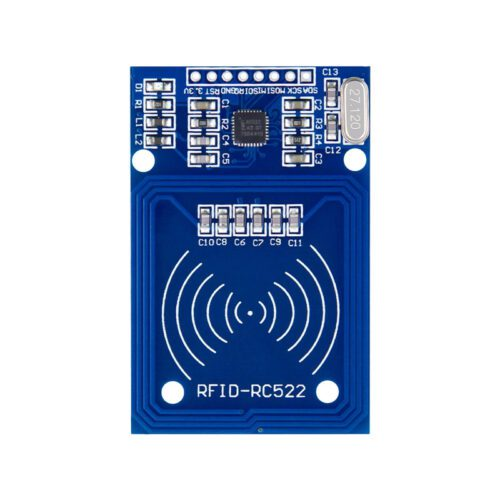
\includegraphics[scale=0.35]{./capitulo_03/figures/HW/rc522.jpg}
\caption{Lector \textit{\acrshort{rfid-acronym}} \label{fig:rc522rf}}
\end{center}
\end{minipage}
\end{figure}

En el ámbito de los sistemas de control de acceso basados en \textit{\acrshort{rfid-acronym}}, diversos trabajos han explorado el uso de estas tecnologías por su facilidad de implementación y capacidad para integrarse en proyectos de \textit{\acrshort{iot-acronym}} y seguridad. Por ejemplo, investigaciones previas \cite{Cherkaoui2021Review, Latifov2023Design} resaltan la viabilidad y flexibilidad de los módulos \textit{\acrshort{rfid-acronym}} en, aplicaciones prácticas.

Para la selección del módulo \textit{\acrshort{rfid-acronym}} más adecuado para el presente proyecto, se consideraron criterios clave como la disponibilidad en el mercado, el costo, la simplicidad de implementación y la compatibilidad con plataformas de desarrollo comunes. A continuación, se presenta la tabla comparativa \ref{fig:tablaRFID}, que incluye tres módulos \textit{\acrshort{rfid-acronym}}: \textit{PN532 NFC RFID Module V3}, \textit{RC522 RFID Module} y \textit{R200 UHF RFID Reader}.

\begin{table}[H]
\centering
\renewcommand{\arraystretch}{1.2} % Ajusta el espacio entre filas
\caption{Tabla comparativa entre módulos \textit{\acrshort{rfid-acronym}}}
\label{fig:tablaRFID}
\begin{tabular}{|p{4.5cm}|p{2.5cm}|p{2.5cm}|p{2.5cm}|}
\hline
\textbf{Criterio / Módulos}                 & \textbf{PN532 NFC RFID Module V3} & \textbf{RC522 RFID Module} & \textbf{R200 UHF RFID Reader} \\ \hline
Disponibilidad en el mercado               & 2                                & 3                          & 1                              \\ \hline
Costo                                      & 2                                & 3                          & 1                              \\ \hline
Simplicidad de implementación              & 2                                & 3                          & 1                              \\ \hline
Compatibilidad con plataformas populares   & 2                                & 3                          & 1                              \\ \hline
Adecuación para pruebas y prototipado      & 2                                & 3                          & 1                              \\ \hline
\textbf{Total}                             & \textbf{10}                      & \textbf{15}                & \textbf{6}                     \\ \hline
\end{tabular}
\end{table}


De acuerdo con los resultados obtenidos en la tabla comparativa, el \textit{RC522 RFID Module} ha sido seleccionado como la opción más adecuada para el proyecto en curso. Su alta disponibilidad, bajo costo y facilidad de implementación lo convierten en el candidato ideal para llevar a cabo pruebas y prototipos. Además, su compatibilidad con plataformas populares como \textit{Arduino} y su sencilla integración en sistemas de control de acceso lo destacan frente a los otros módulos evaluados.

En contraste, aunque el \textit{PN532} ofrece características avanzadas como la compatibilidad \textit{NFC}, su implementación es más compleja. El \textit{R200 UHF}, aunque destaca por su capacidad de lectura a larga distancia, es menos apropiado para un proyecto de bajo costo y prototipado rápido debido a su precio más elevado y la necesidad de antenas externas.

\subsection{Módulo GNSS GP-02 Kit}

El \textit{GP-02-Kit} (ver Figura \ref{fig:gnssgp}) es un módulo de desarrollo altamente integrado que incorpora un receptor de navegación por satélite multimodo de alto rendimiento. El módulo utiliza el chip de posicionamiento por satélite \textit{AT6558R}, el cual combina un frontal de radiofrecuencia, un procesador de banda base digital, una CPU \textit{RISC} de 32 bits, gestión de energía y funciones de detección y protección de antenas activas.

\begin{figure}[H]
\leavevmode
\begin{minipage}{\textwidth}
\begin{center}
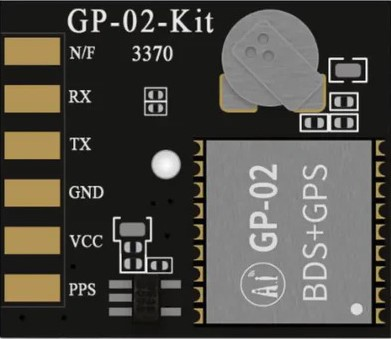
\includegraphics[scale=0.5]{./capitulo_03/figures/HW/GP-02.jpg}
\caption{Módulo de desarrollo \textit{GP-02 Kit} \label{fig:gnssgp}}
\end{center}
\end{minipage}
\end{figure}

Este módulo es compatible con múltiples sistemas de navegación por satélite, incluyendo el sistema de navegación por satélite \textit{BeiDou} de China, el sistema \textit{\acrshort{gps-acronym}} de Estados Unidos y el \textit{GLONASS} de Rusia, lo que le permite realizar un posicionamiento conjunto multi-sistema, garantizando alta precisión en aplicaciones críticas de geolocalización.

El \textit{GP-02-Kit} sigue el protocolo \textit{NMEA} para la transmisión de datos y se comunica con otros dispositivos a través de una interfaz serial \textit{\acrshort{uart-acronym}}, la cual soporta tasas de transferencia de hasta 256000 bps. Además, cuenta con una antena cerámica integrada, lo que simplifica su uso en entornos móviles o aplicaciones de seguimiento donde el tamaño y la eficiencia son esenciales \cite{GP02Kit2021}.

\subsection{Placa de Desarrollo ESP-WROOM-32}

El \textit{ESP32-WROOM-32} (ver Figura \ref{fig:wrom32}) es un módulo \textit{MCU} de alto rendimiento que incluye \textit{Wi-Fi}, \textit{BT} y \textit{\acrshort{ble-acronym}}, ideal para una variedad de aplicaciones, desde redes de sensores de bajo consumo hasta tareas avanzadas como codificación de voz, transmisión de música y decodificación de \textit{MP3}.

En el núcleo de este módulo se encuentra el chip \textit{ESP32-D0WDQ6*}, diseñado para ofrecer escalabilidad y flexibilidad. Posee dos núcleos de \textit{CPU}, controlables individualmente, con una frecuencia de reloj ajustable entre 80 MHz y 240 MHz. Además, permite apagar la \textit{CPU} principal y usar el coprocesador de bajo consumo para monitorear los periféricos de forma constante. Entre sus múltiples periféricos, el \textit{ESP32} integra sensores táctiles capacitivos, sensores \textit{Hall}, interfaz para tarjeta \textit{SD}, \textit{Ethernet}, \textit{\acrshort{spi-acronym}} de alta velocidad, \textit{\acrshort{uart-acronym}}, \textit{\acrshort{i2s-acronym}} e \textit{\acrshort{i2c-acronym}} \cite{Espressif2019}.

Este microcontrolador fue elegido debido a su flexibilidad y disponibilidad, así como por sus capacidades de manejo de periféricos y transmisión de datos, lo que lo convierte en una opción adecuada para las demandas de comunicación en este sistema.

\begin{figure}[H]
\leavevmode
\begin{minipage}{\textwidth}
\begin{center}
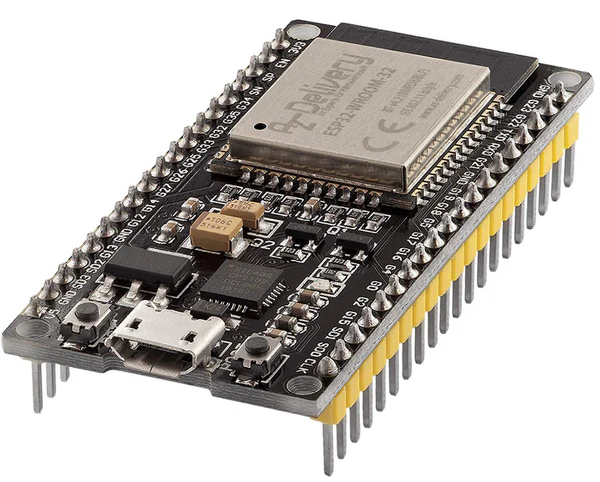
\includegraphics[scale=0.3]{./capitulo_03/figures/HW/wroomp.png}
\caption{Placa de desarrollo \textit{ESP32} \label{fig:wrom32}}
\end{center}
\end{minipage}
\end{figure}


\section{Componentes de \textit{Software}}
Los componentes de software proporcionan las herramientas y entornos de programación necesarios para diseñar, compilar y cargar el código en el hardware. Además, facilitan la visualización de los datos recolectados, permitiendo una supervisión eficiente y en tiempo real del sistema. No solo posibilitan la integración con el hardware, sino que también proporciona una plataforma para interpretar y presentar la información
\subsection{\textit{Helium Console}}
Helium Console es una plataforma desarrollada por Helium que permite la gestión de organizaciones y dispositivos en redes \acrshort{loraw}  a través de una interfaz basada en navegador web. Actúa como un servidor de red \acrshort{loraw} (\acrshort{lns-acronym}, por sus siglas en inglés, \gls{lns-glossary}) compatible con la blockchain de Helium, conocido como Router, que facilita la comunicación entre dispositivos \acrshort{loraw} y la red de Helium. Helium Console simplifica la integración y operación de dispositivos, proporcionando a los usuarios una forma eficiente y directa de administrar sus dispositivos \acrshort{iot-acronym} (Internet of Things, o Internet de las Cosas) dentro de la infraestructura de la red Helium \cite{heliumDocs}.

Una de las principales ventajas de Helium Console es su enfoque “plug-and-play” (lista para usar), lo que significa que los usuarios pueden configurar y operar su propia Organización Única de Identificación (OUI, Organizationally Unique Identifier) en la red Helium de manera rápida y sin necesidad de permisos especiales. Dado que la red de Helium es descentralizada y abierta, la operación de una OUI es completamente permissionless (sin necesidad de permisos), lo que facilita la incorporación de nuevos dispositivos \acrshort{iot-acronym} sin las barreras típicas que se encuentran la mayoria de redes.

Se evaluaron varias plataformas de servidor de red \acrshort{loraw} (\acrshort{lns-acronym}) con el objetivo de elegir la más adecuada para el trabajo. El proceso de selección se basó en analizar criterios específicos que afectan directamente la funcionalidad y adaptabilidad de cada plataforma a los requisitos del proyecto.
\\
Criterios considerados
\begin{itemize}

\item Costo: Considera el gasto involucrado en utilizar la plataforma, desde suscripciones hasta la infraestructura adicional que pueda requerirse. Cuanto menor es el costo, mejor es la evaluación.

\item Facilidad de Uso: Mide la simplicidad y accesibilidad de la interfaz y su curva de aprendizaje, ideal para usuarios con diversos niveles de experiencia.

\item Escalabilidad: Evalúa la capacidad de la plataforma para adaptarse y crecer, tanto en usuarios como en dispositivos, sin que el rendimiento disminuya.

\item Cobertura: Analiza la disponibilidad geográfica de la plataforma y su cobertura en distintas áreas.

\item Control y Personalización: Valora el nivel de control que ofrece la plataforma para adaptar la infraestructura y configuraciones específicas.

\item Privacidad y Seguridad: Mide las medidas de seguridad y cifrado en la transmisión de datos. Mayor puntaje si la plataforma ofrece seguridad avanzada y privacidad de datos.

\item Integración: Evalúa la facilidad de integración de la plataforma con otros sistemas y su capacidad para conectarse con tecnologías \acrshort{iot-acronym}.

\item Documentación: Analiza la calidad y accesibilidad de la documentación proporcionada, indispensable para configurar la plataforma.
 
\end{itemize}

En la tabla \ref{fig:Elec_lns} se comparan plataformas de servidor de red \acrshort{loraw} (\acrshort{lns-acronym}) como: Helium Console, The Things Network (TTN), ChirpStack, Loriot para determinar la plataforma más adecuada.

%\usepackage{tabularx} % Asegúrate de incluir este paquete en el preámbulo
\begin{table}[H]
\centering
\renewcommand{\arraystretch}{1.33} % Ajusta el espacio entre filas
\caption{Comparativa de plataformas LoRaWAN}
\label{fig:Elec_lns}
\begin{tabular}{|p{3cm}|p{2.5cm}|p{2.3cm}|p{2.2cm}|p{1.7cm}|}
\hline
\textbf{Criterios} & \textbf{Helium Console} & \textbf{The Things Network (TTN)} & \textbf{ChirpStack} & \textbf{Loriot} \\ \hline
Costo             & Bueno                   & Excelente                         & Bueno              & Bueno          \\ \hline
Facilidad de Uso  & Excelente               & Excelente                         & Regular            & Excelente      \\ \hline
Escalabilidad     & Excelente               & Regular                           & Bueno              & Bueno          \\ \hline
Cobertura         & Bueno                   & Bueno                             & Regular            & Bueno          \\ \hline
Control y Personalización & Regular        & Regular                           & Excelente          & Bueno          \\ \hline
Privacidad y Seguridad    & Bueno          & Regular                           & Excelente          & Excelente      \\ \hline
Integraciones     & Excelente               & Excelente                         & Excelente          & Bueno          \\ \hline
Documentación     & Excelente               & Excelente                         & Regular            & Excelente      \\ \hline
\end{tabular}
\end{table}


Helium Console destaca principalmente como la opción ganadora debido a su cobertura, un aspecto crucial en el análisis comparativo. Aunque otras plataformas ofrecen excelentes características en varias áreas, Helium sobresale por su capacidad de brindar una red descentralizada y global. Además, otras características como su facilidad de uso, integraciones y documentación excelente también refuerzan su posición.

\subsection{Thingsboard}
ThingsBoard es una plataforma \acrshort{iot-acronym} de código abierto que facilita la recopilación, procesamiento, visualización y  gestión de dispositivos de datos. La plataforma destaca por su capacidad para manejar grandes volúmenes de datos y dispositivos, lo que la convierte en una opción robusta y flexible para diversas aplicaciones en el ámbito de la Internet de las Cosas. Su diseño modular permite a los desarrolladores integrar y gestionar dispositivos de forma eficiente, sin necesidad de construir una infraestructura desde cero.

La arquitectura de ThingsBoard es clave para su funcionalidad, y se puede implementar en dos modalidades: monolítica y microservicios. En su modo monolítico, todos los componentes se ejecutan dentro de una única máquina virtual Java (JVM), optimizando el uso de recursos del sistema operativo y simplificando su implementación en entornos con limitaciones de memoria y procesamiento. Este enfoque centralizado facilita el desarrollo y el prototipado de soluciones \acrshort{iot-acronym}, al requerir menos configuración y memoria. Por otro lado, la modalidad basada en microservicios distribuye los componentes del sistema en nodos independientes, lo que permite una escalabilidad horizontal y una mayor tolerancia a fallos, ideal para proyectos de gran escala donde es crucial gestionar grandes cantidades de dispositivos y datos de manera eficiente. 
La figura \ref{fig:tbarqui} ilustra cómo ThingsBoard organiza sus componentes y cómo interactúan para manejar la comunicación entre dispositivos y sistemas externos \cite{ThingsBoard}.

\begin{figure}[H]
\leavevmode
\begin{minipage}{\textwidth}
\begin{center}
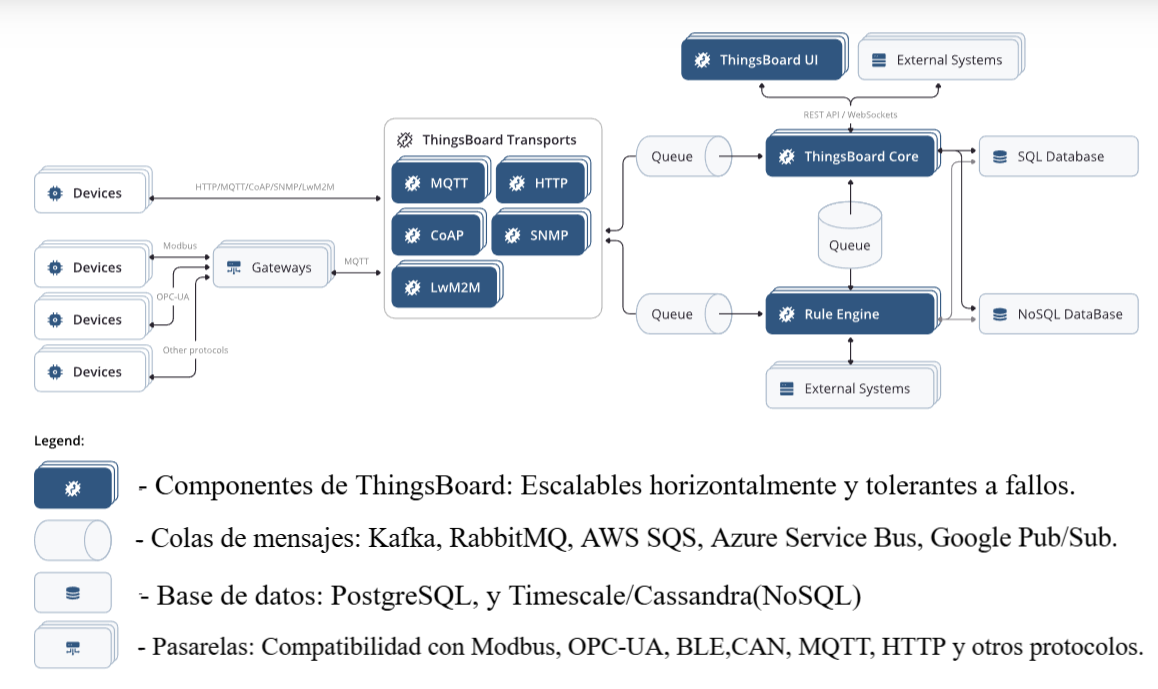
\includegraphics[width=1.0\textwidth]{./capitulo_03/figures/SW/tbarquitecture.png}
\caption{Diagrama de Arquitectura ThingsBoard\label{fig:tbarqui}}
\end{center}
\end{minipage}
\end{figure}

Uno de los componentes esenciales de ThingsBoard es su motor de reglas (Rule Engine), que juega un papel central en la automatización y procesamiento de eventos dentro de la plataforma. Este motor permite procesar los datos entrantes desde los dispositivos \acrshort{iot-acronym} y ejecutar acciones automáticas basadas en la lógica definida por el usuario. El sistema procesa los datos a través de una serie de nodos que realizan diferentes operaciones, como almacenamiento, generación de alertas o control remoto de dispositivos mediante llamadas a procedimientos remotos RPC. Esto posibilita la creación de flujos de trabajo complejos que reaccionan en tiempo real a los eventos generados por los dispositivos, permitiendo a la plataforma tomar decisiones y ejecutar acciones automáticamente sin intervención humana. 
En la Figura \ref{fig:ruleengine} , donde se puede observar cómo se configuran las cadenas de reglas para tomar decisiones basadas en los mensajes recibidos, por ejemplo, enviando comandos de RPC o almacenando datos en bases de datos \cite{ThingsBoard}.

\begin{figure}[H]
\leavevmode
\begin{minipage}{\textwidth}
\begin{center}
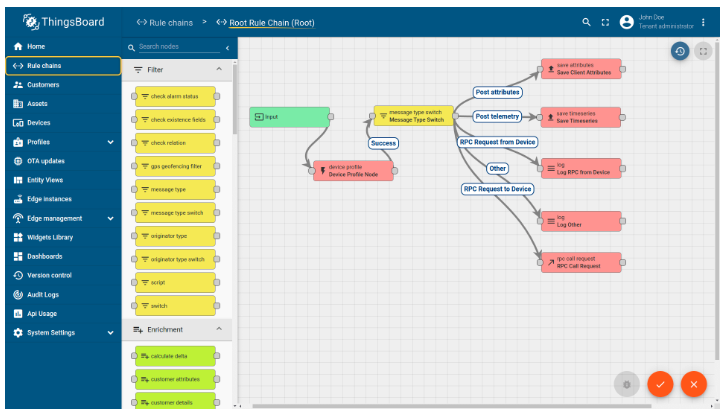
\includegraphics[width=\textwidth]{./capitulo_03/figures/SW/ruleengine.png}
\caption{Cadena de reglas raíz ThingsBoard\label{fig:ruleengine}}
\end{center}
\end{minipage}
\end{figure}

Una visualización adecuada de los datos adquiridos es esencial ya facilita el procesamiento de los mismos, lo que contribuye a la precisión y efectividad de las decisiones tomadas a partir de esta información.  Con el objetivo de facilitar esta visualización y gestión de datos, se seleccionó una plataforma \acrshort{iot-acronym}, basándose en estudios que resaltan el uso de estas herramientas en contextos de monitoreo y análisis de datos \cite{Alquhali2019IOT, Nwankwo2022IoT-Assisted, Santa2019LPWAN-Based, Suwaid2019Embedded, Alavi2019State, K2023IoT}. 

Para determinar la plataforma más adecuada, se evaluaron Ubidots, ThingSpeak y ThingsBoard bajo criterios técnicos relevantes para entornos de prototipado, incluyendo:


\begin{itemize}
    \item Escalabilidad: Este criterio evaluó la capacidad de cada plataforma para manejar un aumento en el número de dispositivos y datos a medida que el proyecto crece.

    \item Protocolos Soportados: Se analizó la diversidad de protocolos de comunicación \acrshort{iot-acronym} que cada plataforma puede gestionar.

    \item Visualización de Datos: Este criterio evaluó la calidad de las herramientas de visualización de datos disponibles en cada plataforma.

    \item Automatización de Reglas: Se evaluó la capacidad de cada plataforma para configurar reglas y flujos de trabajo automáticos.

    \item Costo: Este criterio consideró los costos asociados al uso de las plataformas. 

    \item Soporte y Comunidad: La disponibilidad de soporte técnico y la existencia de una comunidad activa fueron evaluadas. 

    \item Instalación Local (On-Premise): Este criterio evaluó la opción de implementar la plataforma en un servidor propio.

    \item Facilidad de Uso: Finalmente, se evaluó la intuitividad y facilidad de uso de la interfaz para usuarios tanto novatos como avanzados.
\end{itemize}

Cada plataforma fue calificada en una escala de 1 a 3, permitiendo una comparación cuantitativa de sus capacidades, donde:
\begin{itemize}
    \item 1 indica un rendimiento bajo.
    \item 2 un rendimiento medio.
    \item 3 un rendimiento alto.
\end{itemize}

La tabla \ref{fig:Elec_tb} resume los resultados obtenidos, y constituye la base para seleccionar la plataforma que mejor responde a los requerimientos de visualización y control de datos en el proyecto.

\begin{table}[H]
\centering
\renewcommand{\arraystretch}{1.3} % Ajusta el espacio entre filas
\caption{Tabla comparativa de Plataformas IoT}
\label{fig:Elec_tb}
\begin{tabularx}{\textwidth}{|p{4.4cm}|X|X|X|}
\hline
\textbf{Criterio/Plataforma}                & \textbf{Ubidots} & \textbf{ThingSpeak} & \textbf{ThingsBoard} \\ \hline
 Escalabilidad                           & 2                & 2                   & 3                    \\ \hline
 Protocolos Soportados                   & 2                & 2                   & 3                    \\ \hline
 Visualización de Datos                  & 3                & 2                   & 3                    \\ \hline
 Automatización de Reglas                & 2                & 2                   & 3                    \\ \hline
 Costo                                   & 3                & 3                   & 3                    \\ \hline
 Soporte y Comunidad                     & 3                & 3                   & 3                    \\ \hline
 Instalación Local (On-Premise)          & 1                & 1                   & 3                    \\ \hline
 Facilidad de Uso                        & 3                & 3                   & 3                    \\ \hline
\textbf{Total}                             & \textbf{17}      & \textbf{16}         & \textbf{21}          \\ \hline
\end{tabularx}
\end{table}


De acuerdo con los criterios evaluados, ThingsBoard se destaca como la plataforma \acrshort{iot-acronym} más adecuada para el presente proyecto. Su versión Community Edition permite una instalación local sin costos asociados, lo cual resulta especialmente ventajoso en un entorno de prototipado. Además, su capacidad para escalar y su soporte para una amplia gama de protocolos lo convierten en una opción robusta para gestionar y visualizar información en tiempo real. Una de las razones clave para elegir ThingsBoard fue su integración nativa con MQTT \cite{MQTT}, un protocolo ligero que utiliza un modelo de publicación/suscripción para optimizar la transmisión de datos entre dispositivos \acrshort{iot-acronym}. Esto permite una comunicación eficiente, en tiempo real y con bajo consumo de recursos, asegurando la escalabilidad del sistema. Estas características, junto con la posibilidad de uso gratuito y sin limitaciones de licenciamiento comercial, posicionan a ThingsBoard como la solución óptima, permitiendo una implementación sostenible y adaptable.








\subsection{Arduino IDE}

El Arduino IDE o Entorno de Desarrollo Integrado de Arduino, es un entorno de desarrollo integrado que facilita la programación y carga de código en microcontroladores mediante una interfaz amigable \cite{ArduinoIDE}. Permite a los usuarios escribir y editar “sketches” (programas o códigos) en un lenguaje basado en C/C++, simplificado para el control de hardware, lo que agiliza el desarrollo de proyectos de electrónica.

Una de sus ventajas es la flexibilidad en la configuración de hardware, gracias a su “Gestor de Placas” que adapta el código a distintos modelos de microcontroladores y permite la instalación de librerías adicionales. En este proyecto, el Arduino IDE es especialmente útil debido a su compatibilidad con la placa Heltec LoRa WiFi 32 V3, que cuenta con librerías y referencias específicas de Heltec, lo que simplifica la integración de \textit{\acrshort{loraw}} y WiFi.

Además, el IDE permite la carga del código de manera directa desde una conexión USB o inalámbrica, haciendo más ágil el ciclo de pruebas y depuración, gracias a sus herramientas básicas para detectar errores en el código. Estas características hacen del Arduino IDE una opción versátil y eficiente para proyectos con microcontroladores, adecuada para usuarios de todos los niveles.

La interfaz del Arduino IDE se muestra en la Figura \ref{fig:arduino_ide}, donde es posible observar sus principales herramientas para la edición y carga de código.

\begin{figure}[H]
\leavevmode
\begin{minipage}{\textwidth}
\begin{center}
    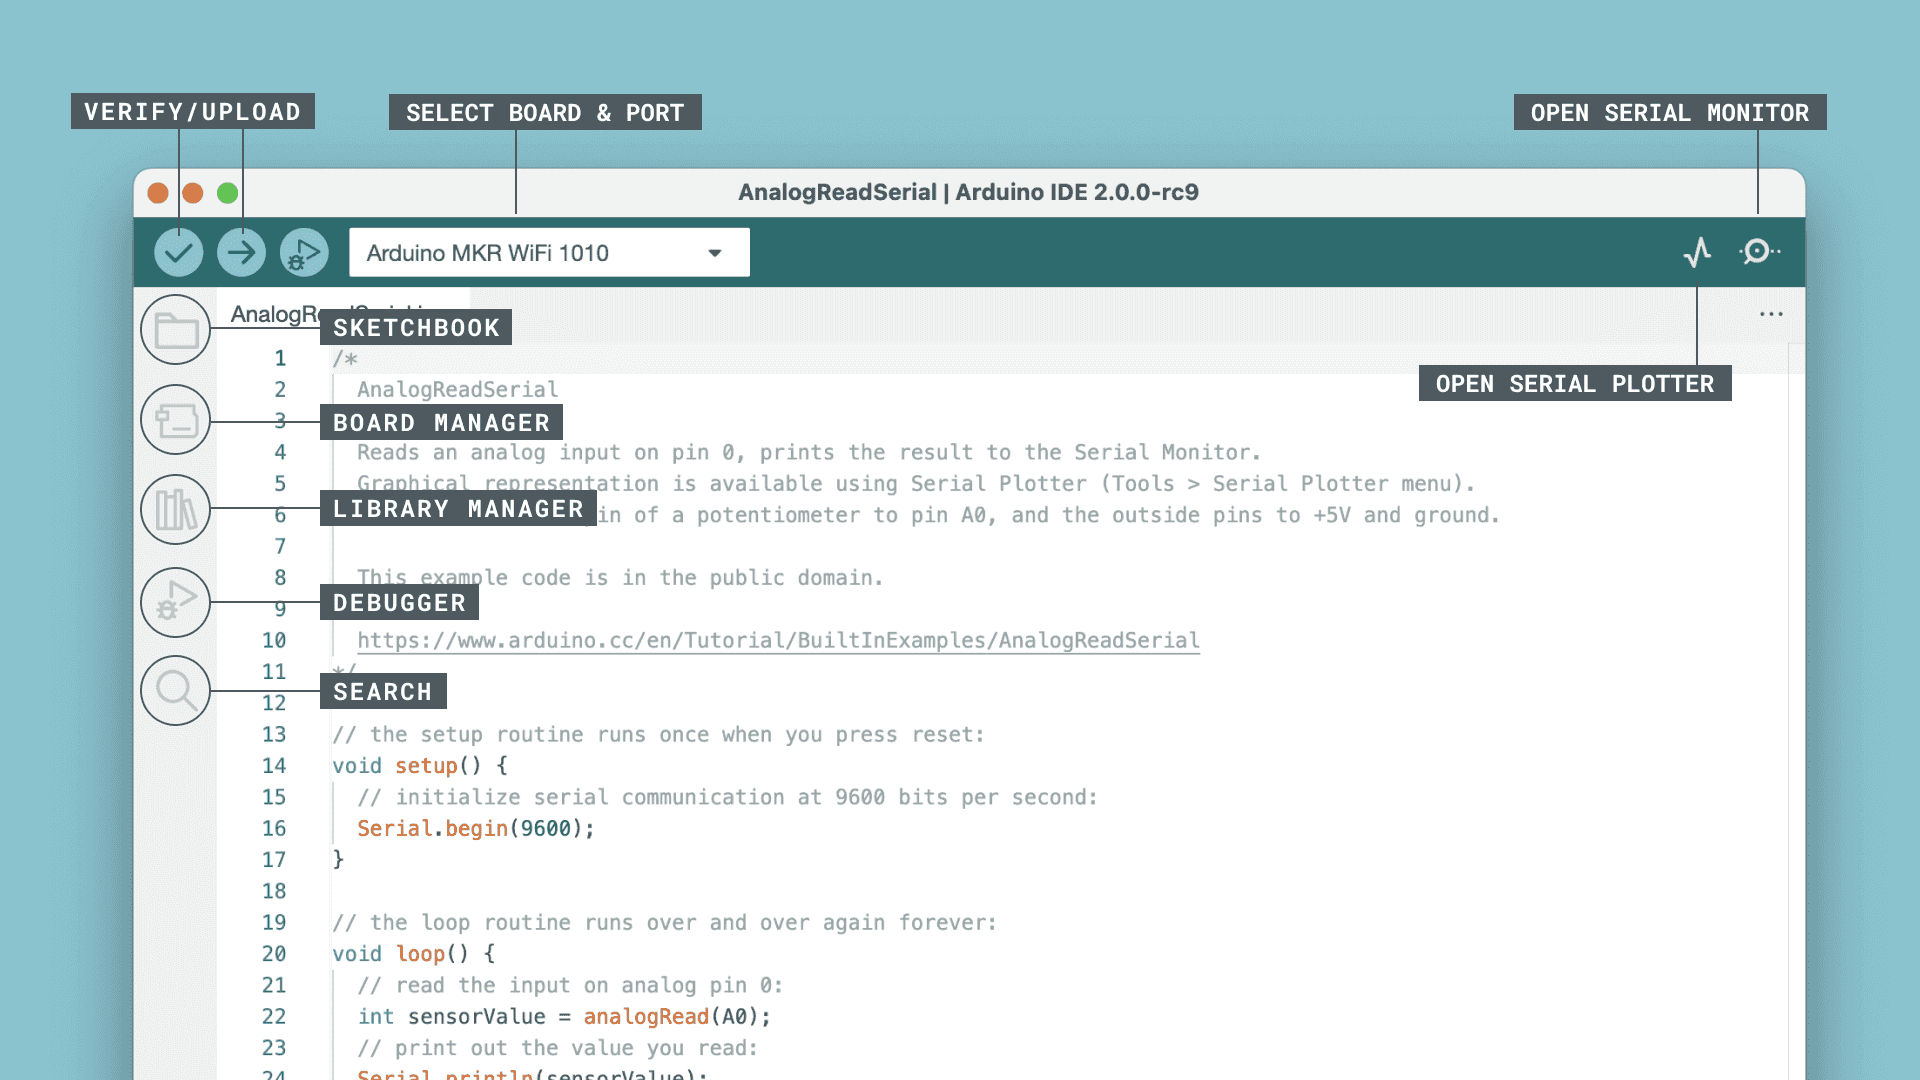
\includegraphics[width=1.0\textwidth]{./capitulo_03/figures/SW/ide-2-ino.png} % Ajusta el tamaño y la ruta de la imagen
    \caption{Interfaz del Arduino IDE 2\cite{ArduinoIDEImage}.}
    \label{fig:arduino_ide}
\end{center}
\end{minipage}
\end{figure}


\subsection{Fritzing}
Fritzing es un software de automatización del diseño electrónico (Electronic Design Automation, EDA) orientado a diseñadores, artistas, investigadores y cualquier persona interesada en la electrónica y el desarrollo de prototipos. Su propósito principal es ofrecer herramientas que faciliten la documentación y el intercambio de proyectos, permitiendo a los usuarios crear y diseñar circuitos de forma visual y accesible \cite{FritzingSoftware}.

El programa se destaca por su interfaz intuitiva, que permite a los usuarios diseñar circuitos, crear esquemas de circuitos impresos y compartir sus prototipos. Además, Fritzing es compatible con otras herramientas de diseño como Processing y Arduino, formando un ecosistema en el que los usuarios pueden documentar y compartir sus proyectos con facilidad. Esto lo convierte en una herramienta valiosa tanto para la enseñanza de electrónica como para la creación de prototipos destinados a la fabricación \cite{FritzingPrimerosPasos}.

La Figura \ref{fig:fritzingf} muestra la interfaz de Fritzing, en la cual es posible visualizar y editar circuitos de manera sencilla y gráfica. Este entorno facilita tanto el diseño de circuitos como la creación de esquemas listos para fabricación, adaptándose a las necesidades de diversos usuarios y proyectos.

\begin{figure}[H]
\leavevmode
\begin{minipage}{\textwidth}
\begin{center}
    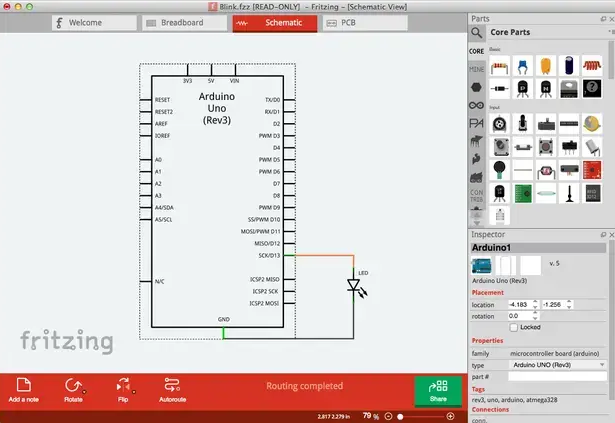
\includegraphics[width=0.7\textwidth]{./capitulo_03/figures/SW/fritzing.png} % Ajusta el tamaño y la ruta de la imagen
    \caption{Entorno de diseño de Fritzing mostrando el esquema de una placa\cite{FritzingPrimerosPasos}.}
    \label{fig:fritzingf}
\end{center}
\end{minipage}
\end{figure}



\subsection{Blender}

Blender es una suite de creación 3D gratuita y de código abierto que soporta toda la cadena de producción 3D: modelado, rigging, animación, simulación, renderizado, composición, seguimiento de movimiento, edición de video e incluso creación de juegos. Los usuarios avanzados pueden utilizar la \acrshort{api-acronym} de Blender para scripting en Python, permitiendo personalizar la aplicación y desarrollar herramientas especializadas que a menudo se incluyen en futuras versiones.

Una de las grandes ventajas de Blender es su accesibilidad y versatilidad. Al ser gratuito y estar disponible para múltiples plataformas como Linux, Windows y macOS, permite que tanto individuos como pequeños estudios accedan a herramientas profesionales sin incurrir en altos costos. Su interfaz unificada y el uso de OpenGL garantizan una experiencia consistente en todos los sistemas operativos \cite{Blender}.

Además, Blender es impulsado por una comunidad activa bajo la Licencia Pública General de GNU (GPL), lo que significa que cualquier persona puede contribuir al desarrollo del software. Esto conduce a la incorporación constante de nuevas funciones, correcciones rápidas de errores y mejoras en la usabilidad. La colaboración comunitaria fomenta la innovación y asegura que el software evolucione para satisfacer las necesidades cambiantes de sus usuarios \cite{Blender1}.

Blender no solo ofrece una solución completa para la creación de contenido 3D, sino que también promueve un entorno colaborativo y abierto. Su combinación de potencia, flexibilidad y gratuidad lo convierte en una opción ideal para aquellos que buscan desarrollar proyectos creativos sin las limitaciones de los software propietarios.

 En la figura \ref{fig:blender}, se muestra la interfaz de Blender, donde es posible dibujar directamente en una ventana gráfica 3D. Esta funcionalidad abre una libertad de flujo de trabajo sin igual para creadores de guiones gráficos y artistas 2D. Blender permite combinar elementos 2D y 3D directamente en la ventana gráfica. Además, incluye capas y colores para trazos y rellenos, así como la capacidad de esculpir pinceladas y asociarlas a objetos 3D.


 \begin{figure}[H]
\leavevmode
\begin{minipage}{\textwidth}
\begin{center}
    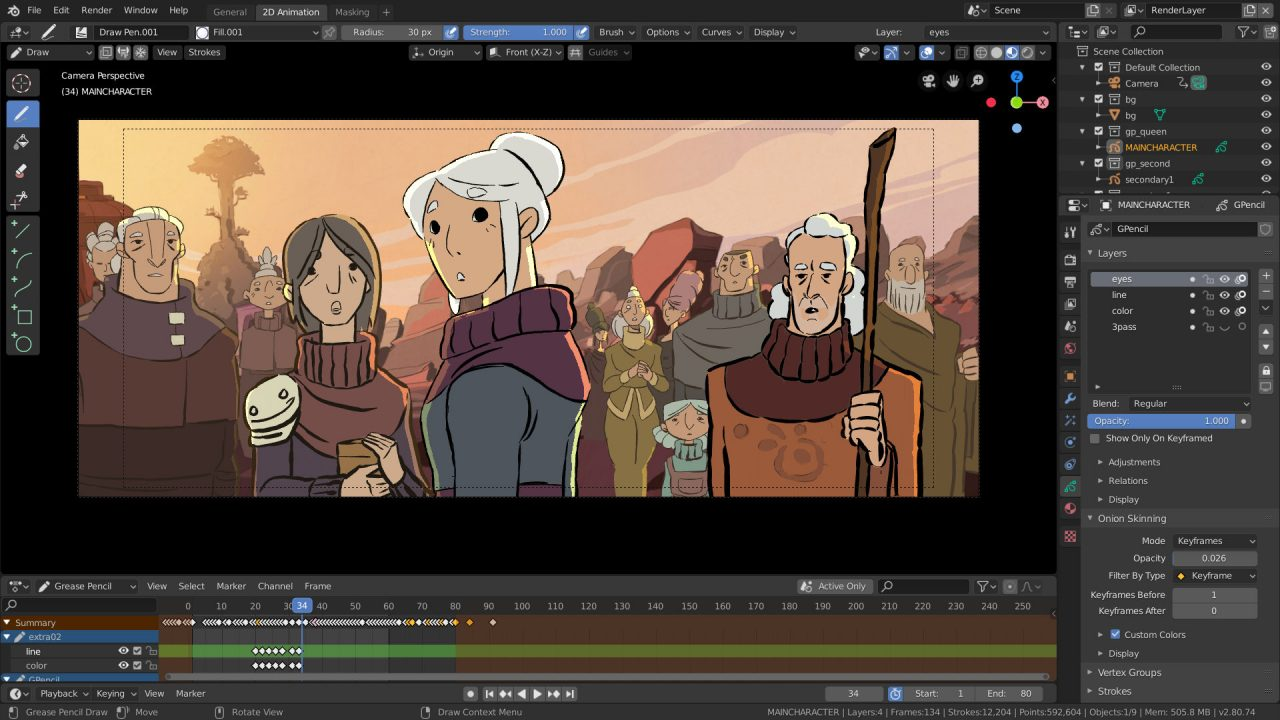
\includegraphics[width=0.7\textwidth]{./capitulo_03/figures/SW/herojpg.jpg} % Ajusta el tamaño y la ruta de la imagen
    \caption{Entorno de desarrollo en Blender.}
    \label{fig:blender}
\end{center}
\end{minipage}
\end{figure}
\fancyhead{}
\fancyfoot{}
\pagestyle{plain}

\lhead{Método}

\chapter{Método}

Este capítulo describe el desarrollo del trabajo de investigación, enfocado en la creación de un prototipo de control para motocicletas mediante tecnologías \textit{\acrshort{rfid-acronym}} y \textit{\acrshort{loraw}}, con el propósito de implementar un sistema de autenticación y localización para prevenir robos. El trabajo constituye una investigación aplicada al desarrollo tecnológico de un sistema de seguridad antirrobo, con un enfoque cuantitativo y un diseño experimental y transversal en el tiempo, abarcando el desarrollo de un prototipo funcional. En las siguientes secciones se detallan los módulos desarrollados, cada uno representando una fase clave en el funcionamiento del sistema (ver Figura \ref{modulo}).

\begin{figure}[H]
    \centering
    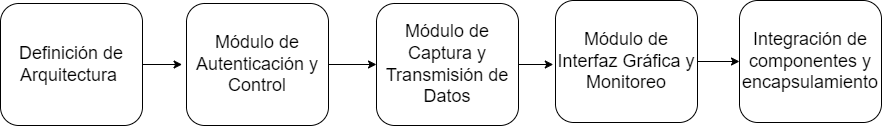
\includegraphics[width=\textwidth]{./capitulo_04/imagen/modulos.drawio.png}
    \caption{Fases principales del sistema.}
    \label{modulo}
\end{figure}

\section{Definición de arquitectura}

En esta primera fase, se definieron los requisitos técnicos orientados a proporcionar seguridad y monitoreo remoto en tiempo real mediante tecnologías \textit{IoT}. El objetivo principal fue desarrollar un sistema que autentique al propietario de la motocicleta a través de un módulo \textit{\acrshort{rfid-acronym}} y, en caso de intento de robo o alejamiento del vehículo sin el \textit{tag} autorizado, interrumpa el encendido y envíe una alerta a un servidor remoto. Para satisfacer estos requisitos, se diseñó una arquitectura que integra comunicación de baja potencia mediante \textit{\acrshort{loraw}} y un dispositivo de geolocalización \textit{\acrshort{gnss-acronym}}, permitiendo el monitoreo y la visualización de datos en una plataforma gráfica accesible.

\subsection{Requisitos clave}

\begin{itemize}
    \item Autenticación del propietario mediante \textit{\acrshort{rfid-acronym}}.
    \item Corte de corriente en el sistema de encendido de la motocicleta cuando el \textit{tag} autorizado se encuentre fuera de rango.
    \item Envío de datos de geolocalización (coordenadas \textit{\acrshort{gnss-acronym}}) y estado de autenticación mediante \textit{\acrshort{loraw}} hacia la red Helium.
    \item Monitoreo remoto de la ubicación y estado de la motocicleta a través de una interfaz gráfica.
\end{itemize}

Con base en estos requisitos, se definieron dos aspectos principales: la estructura interna del prototipo y la arquitectura de comunicación externa hacia el servidor. 

\subsection{Estructura interna del prototipo}

La Figura \ref{fig:diagrama1} ilustra el diseño del hardware y el flujo de control dentro del prototipo.

\begin{figure}[H]
\leavevmode
\begin{minipage}{\textwidth}
\begin{center}
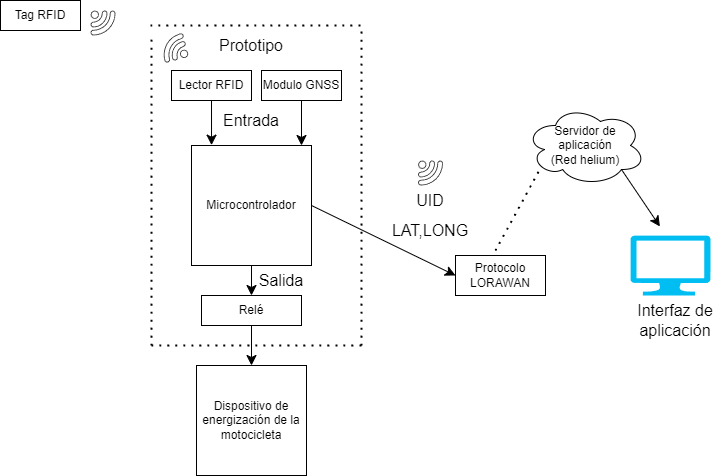
\includegraphics[scale=0.5]{./capitulo_04/imagen/diagrama1.png}
\caption{Estructura del prototipo. \label{fig:diagrama1}}
\end{center}
\end{minipage}
\end{figure}

\begin{itemize}
    \item \textbf{Microcontrolador (Heltec WiFi LoRa 32 V3):} Procesa las entradas de los módulos \textit{\acrshort{rfid-acronym}} y \textit{\acrshort{gnss-acronym}}, y envía datos mediante \textit{\acrshort{loraw}}.
    \item \textbf{Módulo \textit{\acrshort{rfid-acronym}}:} Detecta y autentica el \textit{tag} del usuario. Si el \textit{UID} del \textit{tag} coincide con uno de los usuarios autorizados, se habilita el sistema de arranque.
    \item \textbf{Módulo \textit{\acrshort{gnss-acronym}}:} Proporciona las coordenadas de geolocalización, que se envían junto con el \textit{UID} autenticado para monitoreo remoto.
    \item \textbf{Relé:} Controla el flujo de energía hacia el encendido de la motocicleta. Si el \textit{tag \acrshort{rfid-acronym}} no es reconocido o se retira del rango, el relé corta la energía, evitando que la motocicleta arranque.
\end{itemize}

\subsection{Arquitectura de comunicación externa}

La Figura \ref{fig:diagrama2} muestra cómo los datos capturados por el prototipo se procesan para cumplir con los requisitos de monitoreo remoto en tiempo real.

\begin{figure}[H]
\leavevmode
\begin{minipage}{\textwidth}
\begin{center}
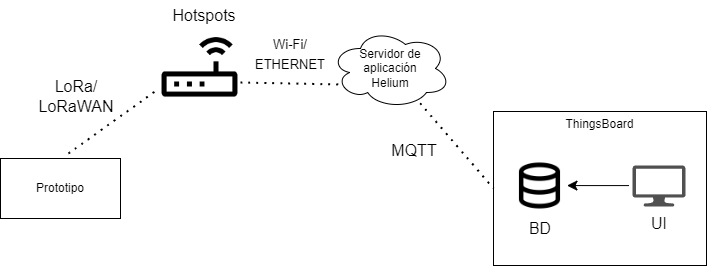
\includegraphics[scale=0.5]{./capitulo_04/imagen/diagrama2.png}
\caption{Arquitectura de comunicación y monitoreo. \label{fig:diagrama2}}
\end{center}
\end{minipage}
\end{figure}

\begin{itemize}
    \item \textbf{Prototipo:} Recopila datos del \textit{\acrshort{rfid-acronym}} y las coordenadas \textit{\acrshort{gnss-acronym}}. El microcontrolador envía esta información utilizando el protocolo \textit{\acrshort{loraw}}.
    \item \textbf{\textit{Hotspots Helium}:} Actúan como puntos de acceso, recibiendo los datos enviados por el prototipo y transmitiéndolos al servidor de aplicación.
    \item \textbf{Servidor Helium:} Procesa los datos recibidos y los envía mediante el protocolo \textit{MQTT} a la plataforma \textit{ThingsBoard}.
    \item \textbf{\textit{ThingsBoard (UI):}} Plataforma que permite la visualización gráfica de los datos en tiempo real. Los usuarios pueden monitorear la ubicación de la motocicleta, su estado de autenticación, y recibir alertas en caso de eventos inusuales, como intentos de robo.
\end{itemize}


\section{Módulo de autenticación y control}

En esta fase, se desarrollaron las funciones principales para garantizar la autenticación del usuario antes de permitir el arranque de la motocicleta. El sistema está diseñado para validar la presencia de un \textit{tag \acrshort{rfid-acronym}} autorizado; solo cuando se detecta un \textit{tag} registrado se permite el arranque del motor de la motocicleta. Si el \textit{tag} no es detectado o es removido en algún momento, el sistema corta el suministro de corriente al motor, bloqueando su funcionamiento. Este mecanismo proporciona una primera capa de seguridad para prevenir el uso no autorizado de la motocicleta.

\subsection{Requisitos del sistema}

Para implementar esta funcionalidad, se definieron los siguientes requisitos:

\begin{itemize}
    \item \textbf{Comparación de UID:} El sistema debe comparar el UID del \textit{tag} detectado con una lista de UID autorizados.
    \item \textbf{Verificación en rango:} Una vez autorizado el \textit{tag}, el sistema realiza una lectura constante para verificar que el \textit{tag} permanezca en rango.
\end{itemize}

Considerando estos requisitos, se diseñó el diagrama de flujo que representa el funcionamiento del sistema de autenticación y control (Figura \ref{fig:rfid1}).

\begin{figure}[H]
    \centering
    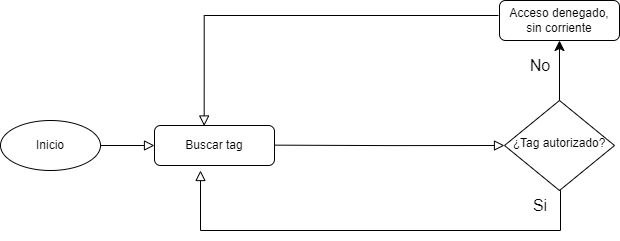
\includegraphics[scale=0.5]{./capitulo_04/imagen/diagramadeflujoRFID-Page-1.drawio.png}
    \caption{Diagrama de flujo de autenticación y control.}
    \label{fig:rfid1}
\end{figure}

\subsection{Conexión del módulo \textit{RFID}}

Para la comunicación entre el módulo \textit{RFID RC522} y la placa de desarrollo \textit{WiFi LoRa 32 V3} se empleó el protocolo SPI. Los pines de conexión utilizados fueron: 
\begin{itemize}
    \item \textbf{CS:} Pin 34.
    \item \textbf{MOSI:} Pin 35.
    \item \textbf{CLK:} Pin 36.
    \item \textbf{MISO:} Pin 26.
    \item \textbf{RESET:} Pin 33.
    \item \textbf{VCC y GND:} Pines de alimentación.
\end{itemize}

En la Figura \ref{fig:conexionrfid} se muestra el diagrama de conexiones utilizadas para esta configuración.

\begin{figure}[H]
\leavevmode
\begin{minipage}{\textwidth}
\begin{center}
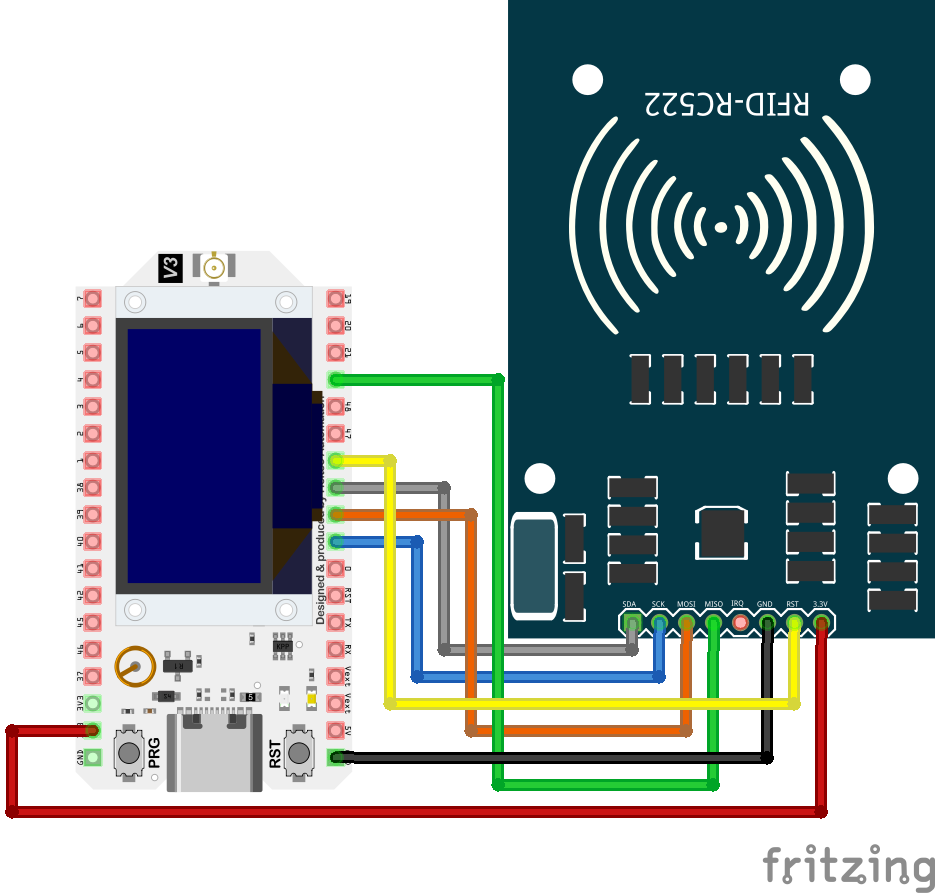
\includegraphics[scale=0.8]{./capitulo_04/imagen/diagramaRFID.png}
\caption{Diagrama de conexiones entre WiFi LoRa 32 V3 y RFID RC522. \label{fig:conexionrfid}}
\end{center}
\end{minipage}
\end{figure}

\subsection{Primera versión del código: implementación básica en el bucle principal}

La primera versión del código implementa un sistema de autenticación y monitoreo continuo de un \textit{tag \acrshort{rfid-acronym}}, permitiendo el acceso únicamente cuando se detecta la presencia de un \textit{tag} autorizado. En este caso, se definieron dos UIDs correspondientes a \textit{Usuario1} y \textit{Usuario2}. Al leer el UID del \textit{tag}, el sistema lo compara con estos valores autorizados para conceder o denegar el acceso.

\subsubsection{Autenticación del \textit{tag}}
\begin{itemize}
    \item Si \texttt{tagAutenticada} es \texttt{falso}, el sistema permanece en espera, buscando la presencia de un \textit{tag \acrshort{rfid-acronym}}.
    \item Cuando se detecta un \textit{tag}, se lee su UID y se utiliza la función \texttt{comparaUID()} para verificar si coincide con uno de los usuarios autorizados. Si coincide, se muestra un mensaje de bienvenida y \texttt{tagAutenticada} se establece en \texttt{verdadero}.
    \item Si el UID no es reconocido, se muestra un mensaje indicando que el \textit{tag} no es válido.
\end{itemize}

\subsubsection{Verificación de presencia del \textit{tag}}
\begin{itemize}
    \item Si \texttt{tagAutenticada} es \texttt{verdadero}, el sistema verifica constantemente si el \textit{tag} autorizado permanece en rango.
    \item Si el tiempo desde la última detección del \textit{tag} excede un límite definido (\texttt{tiempoCorte}), el sistema corta el suministro de corriente al motor.
    \item Si el \textit{tag} sigue en rango, se actualiza el tiempo de última lectura y el motor continúa en funcionamiento.
\end{itemize}

\subsection{Segunda versión del código: integración de FreeRTOS y modularización}

En esta versión, se incorporó \gls{rtos} para gestionar de manera concurrente la autenticación del \textit{tag \acrshort{rfid-acronym}} y la verificación de su presencia. Además, el código se modularizó en archivos específicos para facilitar su mantenimiento y escalabilidad:

\begin{itemize}
    \item \textbf{Archivo \texttt{rfidfunciones.h}:} Declaraciones de variables y funciones relacionadas con el módulo \textit{\acrshort{rfid-acronym}}.
    \item \textbf{Archivo \texttt{rfidfunciones.cpp}:} Implementación de funciones y tareas de FreeRTOS para autenticación y monitoreo.
    \item \textbf{Archivo principal \texttt{RFIDFreeRTOS.ino}:} Inicialización de tareas de FreeRTOS y configuración de parámetros principales.
\end{itemize}

\subsubsection{Tareas implementadas con FreeRTOS}

\paragraph{Tarea 1: \texttt{tareaDeteccionTag}}
\begin{itemize}
    \item Busca la presencia de un \textit{tag \acrshort{rfid-acronym}}. Si se detecta, verifica su autenticidad mediante la función \texttt{autenticarTag()}.
    \item Monitorea la permanencia del \textit{tag} en rango. Si el \textit{tag} es detectado nuevamente, actualiza el tiempo de última lectura.
    \item Notifica a la tarea de verificación del tiempo mediante un semáforo (\texttt{tagDetectadaSemaphore}).
\end{itemize}

\paragraph{Tarea 2: \texttt{tareaVerificarTiempo}}
\begin{itemize}
    \item Espera la señal del semáforo para ejecutar la función \texttt{verificarTiempo()}, que comprueba si el tiempo transcurrido desde la última detección supera el límite definido (\texttt{tiempoCorte}).
    \item Si el tiempo excede el límite, se corta el suministro de corriente y se establece \texttt{tagAutenticada} en \texttt{falso}.
\end{itemize}

Esta versión proporciona una estructura modular, mejorando la eficiencia y permitiendo un control más preciso del sistema. El uso de \textit{FreeRTOS} optimiza la gestión de tareas críticas, asegurando la sincronización y escalabilidad del sistema.


\section{Módulo de captura y transmisión de datos}

Para llevar a cabo la captura y transmisión de datos en tiempo real, se desarrollaron códigos específicos que permiten la adquisición de coordenadas de ubicación mediante el módulo \textit{\acrshort{gnss-acronym}} y su transmisión eficiente a través de \textit{\acrshort{loraw}}, integrando ambos subsistemas en el funcionamiento general del prototipo.

Este proceso se dividió en tres fases:

\begin{itemize}
    \item Implementación básica para obtención de datos de las coordenadas en tiempo real.
    \item Implementación y configuración del módulo \textit{\acrshort{loraw}} para la transmisión de datos.
    \item Integración de la comunicación entre los módulos \textit{\acrshort{gnss-acronym}} y \textit{\acrshort{loraw}}.
\end{itemize}

Para la comunicación entre el módulo \textit{\acrshort{gnss-acronym}} y la placa de desarrollo \textit{WiFi LoRa 32 V3}, se empleó el protocolo \textit{UART}. Los pines de conexión utilizados fueron el pin 45 (RX), pin 46 (TX), y los pines de alimentación \textit{VCC} y \textit{GND}. En la Figura \ref{fig:conexionGNSS}, se muestra el diagrama de conexiones utilizado.

\begin{figure}[H]
    \leavevmode
    \begin{minipage}{\textwidth}
    \begin{center}
    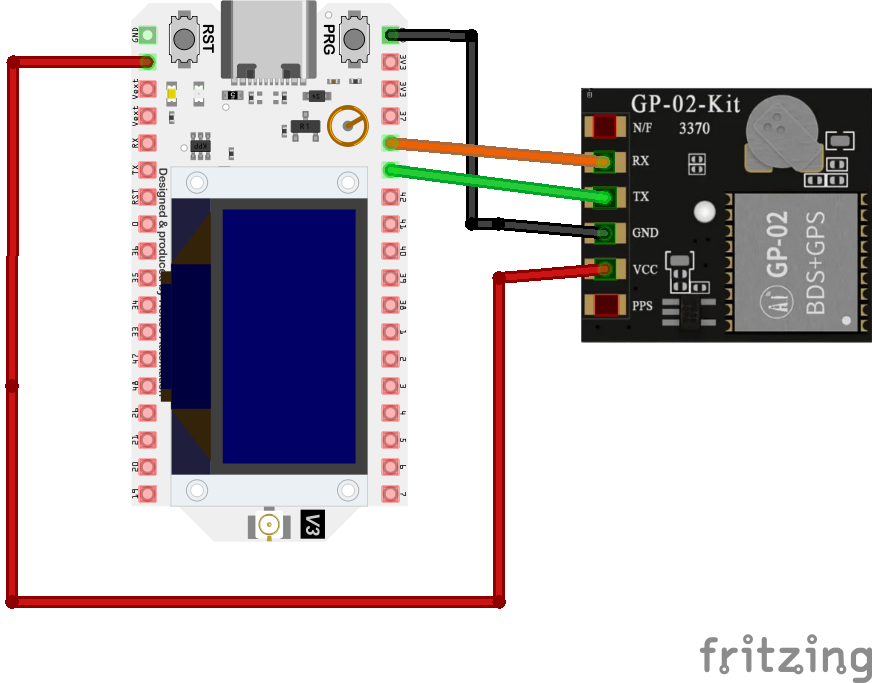
\includegraphics[scale=0.8]{./capitulo_04/imagen/diagramaGNSS.png}
    \caption{Diagrama de conexiones entre \textit{WiFi LoRa 32 V3} y \textit{\acrshort{gnss-acronym}}. \label{fig:conexionGNSS}}
    \end{center}
    \end{minipage}
\end{figure}

\subsection{Implementación básica para obtención de datos de las coordenadas en tiempo real}

Una vez conectado el módulo \textit{\acrshort{gnss-acronym}} a la placa de desarrollo, se implementó un código para obtener y mostrar en tiempo real los datos de ubicación (latitud y longitud), junto con la fecha y hora actual. Este código se basa en la librería \textit{TinyGPSPlus}, que permite interpretar los datos en formato \textit{NMEA} recibidos desde el GPS. A continuación, se describe la implementación:

\subsubsection{Función \texttt{setup()}}
Durante la fase de inicialización, la función \texttt{setup()} se encarga de:
\begin{itemize}
    \item Configurar el monitor serial (\texttt{Serial}) a 115200 baudios para facilitar la visualización de los datos en una terminal serial.
    \item Configurar \texttt{Serial1}, el puerto serial dedicado a la comunicación con el GPS, con los pines y velocidad previamente definidos.
\end{itemize}

\subsubsection{Proceso de captura de datos en la función \texttt{loop()}}

En la función \texttt{loop()}, el sistema verifica continuamente si hay datos disponibles en el puerto \texttt{Serial1}, donde el módulo \textit{GPS} envía sus mensajes de datos. El flujo de trabajo en esta función es el siguiente:

\paragraph{Recepción y decodificación de datos:}
\begin{itemize}
    \item Cuando \texttt{Serial1} tiene datos disponibles, estos se procesan utilizando la función \texttt{gps.encode()}. Esta función decodifica los mensajes de datos en formato \textit{NMEA} provenientes del \textit{GPS} y almacena la información en la instancia \texttt{gps} de la clase \textit{TinyGPSPlus}.
\end{itemize}

\paragraph{Verificación de la validez de los datos:}
\begin{itemize}
    \item Si \texttt{gps.encode()} detecta un mensaje completo de datos \textit{GPS} válido, se llama a la función \texttt{displayInfo()}, que muestra los datos procesados (ubicación, fecha y hora) en el monitor serial.
    \item Si no se reciben suficientes caracteres de \textit{GPS} dentro de los primeros 5 segundos (menos de 10 caracteres), se muestra un mensaje de error en el monitor serial indicando que no se detecta el \textit{GPS}. Esto podría deberse a un problema de cableado, en cuyo caso el sistema se detiene para evitar lecturas incorrectas.
\end{itemize}

\subsubsection{Función \texttt{displayInfo()}}

La función \texttt{displayInfo()} se encarga de presentar los datos de ubicación, fecha y hora en el monitor serial.

\paragraph{Visualización de la ubicación (latitud y longitud):}
\begin{itemize}
    \item Si los datos de ubicación son válidos (\texttt{gps.location.isValid()}), se muestran la latitud y longitud con una precisión de hasta seis decimales. Esta precisión permite obtener coordenadas exactas del dispositivo en el mapa.
    \item Si los datos no son válidos, se muestra el mensaje “\texttt{INVALIDO}” en lugar de las coordenadas.
\end{itemize}

\paragraph{Visualización de la fecha:}
\begin{itemize}
    \item Si el \textit{GPS} proporciona una fecha válida (\texttt{gps.date.isValid()}), esta se presenta en formato \texttt{MM/DD/AAAA}.
    \item Si la fecha no es válida o no se ha recibido, se muestra “\texttt{INVALIDO}” en su lugar.
\end{itemize}

\paragraph{Visualización de la hora:}
\begin{itemize}
    \item La hora se muestra en formato \texttt{HH:MM:SS.CC} (horas, minutos, segundos y centésimas de segundo) si los datos son válidos (\texttt{gps.time.isValid()}).
    \item Si la hora no es válida, se muestra “\texttt{INVALIDO}”.
\end{itemize}



\subsection{Implementación y configuración del módulo \acrshort{loraw} para la transmisión de datos}

En esta fase, se llevó a cabo la configuración del sistema de transmisión de datos mediante la consola \textit{Helium (Legacy)} \cite{Helium_Console}, junto con la placa de desarrollo Heltec WiFi LoRa 32 V3. A continuación, se detallan los pasos y configuraciones necesarios para establecer la comunicación entre el dispositivo y la red \textit{Helium}, así como los procesos requeridos para su correcto funcionamiento.

\subsubsection{Uso de la consola \textit{Helium}}
La consola \textit{Helium} se empleó para configurar los parámetros de los nodos, verificar el estado de la red y monitorear las transmisiones de datos. A través de esta plataforma, se prepararon los entornos necesarios para visualizar la conectividad entre los dispositivos y la consola, incluyendo el registro de los dispositivos y la verificación de su comunicación con los \textit{gateways}.

El proceso comenzó con el acceso a una organización en la que se habían otorgado permisos de usuario. Tras recibir estos permisos, se procedió a crear una cuenta en la plataforma \textit{Helium}. Completado el registro y acceso a la cuenta, fue posible crear un nodo en la red \textit{Helium}, configurado específicamente para recibir los datos transmitidos por el dispositivo. La Figura \ref{fig:helium} ilustra el entorno de configuración en la consola \textit{Helium}, donde se han resaltado con recuadros negros los elementos clave, incluyendo las credenciales principales necesarias para establecer la conexión.

\begin{figure}[H]
\leavevmode
\begin{minipage}{\textwidth}
\begin{center}
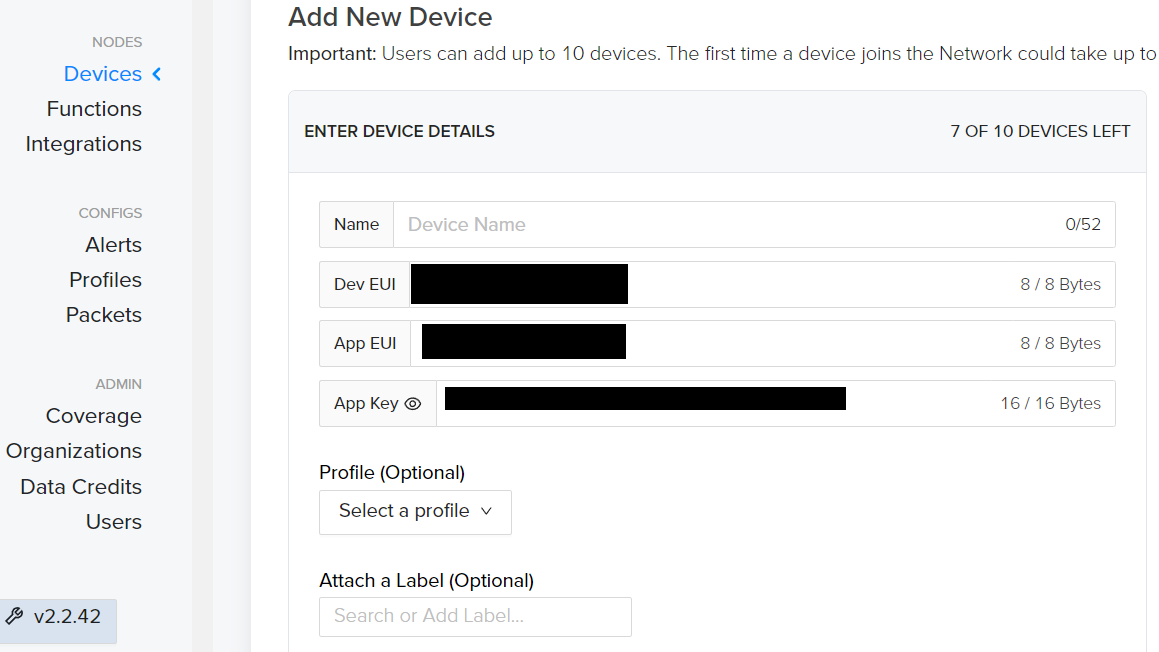
\includegraphics[width=\textwidth]{./capitulo_04/imagen/helium.png}
\caption{Entorno para crear dispositivo y configuración de las credenciales necesarias para el nodo. \label{fig:helium}}
\end{center}
\end{minipage}
\end{figure}

\subsubsection{Configuración del dispositivo Heltec WiFi LoRa 32 V3}

Luego de crear el nodo y obtener las credenciales necesarias, el siguiente paso fue la configuración de la placa de desarrollo Heltec WiFi LoRa 32 V3. Para la implementación inicial, se utilizó la documentación oficial de \textit{Heltec Automation} \cite{heltec}, que proporciona instrucciones detalladas paso a paso sobre la configuración del módulo \textit{\acrshort{loraw}}, así como las librerías requeridas para su funcionamiento.

Una vez completada esta configuración, se consultó la guía oficial de \textit{Helium} \cite{heliumDocs1}, para su integración en el entorno Arduino IDE, adaptándola a las especificaciones particulares de la placa. Esta guía proporcionó los pasos necesarios para registrar las credenciales generadas, permitiendo que el dispositivo enviara datos en \textit{uplink} a la red \textit{Helium}. En la Figura \ref{fig:dispositivo}, se muestran los ajustes de los parámetros necesarios para la comunicación con el servidor \textit{\acrshort{loraw}}.

\begin{figure}[H]
\leavevmode
\begin{minipage}{\textwidth}
\begin{center}
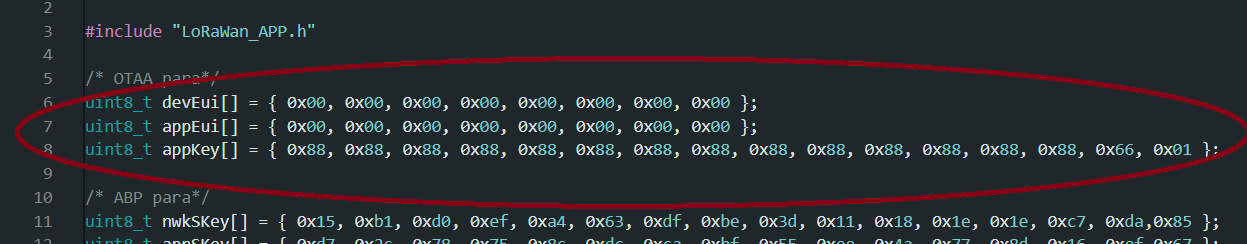
\includegraphics[width=\textwidth]{./capitulo_04/imagen/otta.png}
\caption{Ajuste de los parámetros necesarios en el dispositivo para la comunicación con el servidor \textit{\acrshort{loraw}}. \label{fig:dispositivo}}
\end{center}
\end{minipage}
\end{figure}


\subsection{Implementación de la comunicación entre los módulos\textit{\acrshort{gnss-acronym}} y \textit{\acrshort{loraw}}}

Una vez configurados y validados de manera independiente tanto el módulo \textit{\acrshort{gnss-acronym}} como el sistema de comunicación \textit{\acrshort{loraw}}, se procedió con la integración de ambos componentes. El objetivo de esta fase fue garantizar que las coordenadas obtenidas por el módulo \textit{\acrshort{gnss-acronym}} se transmitieran de manera eficiente a través de la red \textit{\acrshort{loraw}}. Para ello, se realizaron los ajustes necesarios en el código, asegurando que la captura de los datos de ubicación y su envío a través de \textit{\acrshort{loraw}} ocurrieran de manera sincronizada y sin pérdida de información.

En esta sección, se describen en detalle los procesos y el funcionamiento del código ajustado para integrar los sistemas de geolocalización y transmisión de datos.

Como primer paso, se diseñó un diagrama de flujo para representar el funcionamiento del sistema integrado, el cual se puede observar en la Figura \ref{fig:flujo}.

\begin{figure}[H]
\leavevmode
\begin{minipage}{\textwidth}
\begin{center}
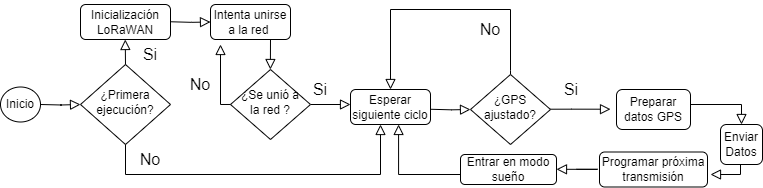
\includegraphics[width=\textwidth]{./capitulo_04/imagen/diagramadeflujognss.png}
\caption{Diagrama de flujo de transmisión de datos por \textit{\acrshort{loraw}}. \label{fig:flujo}}
\end{center}
\end{minipage}
\end{figure}

Una vez diseñado el diagrama de flujo, se procedió a desarrollar una nueva versión del código, reutilizando los fragmentos de código de las fases anteriores e incorporando los ajustes necesarios. A continuación, se describe la implementación de este código.

El programa inicia con la inclusión de las librerías esenciales: \texttt{\acrshort{loraw}APP.h}, para gestionar la comunicación mediante \textit{\acrshort{loraw}}, y \texttt{TinyGPSPlus.h}, para manipular los datos obtenidos del módulo \textit{\acrshort{gnss-acronym}}. Luego, se configuran los pines de acuerdo con las definiciones establecidas en la primera fase del proyecto.

A continuación, se definen los parámetros de conexión de \textit{\acrshort{loraw}}. La conexión puede configurarse de dos maneras: mediante \textit{\acrshort{otaa-acronym}} (\textit{\gls{otaa-glossary}}) o \textit{ABP} (\textit{Activation By Personalization}). Para ello, se especifican las claves necesarias para cada método (\texttt{devEui}, \texttt{appEui}, \texttt{\acrshort{appkey-acronym}} para \textit{\acrshort{otaa-acronym}}, y \texttt{\acrshort{nwkskey-acronym}}, \texttt{\acrshort{appskey-acronym}}, \texttt{devAddr} para \textit{ABP}). También se definen los canales de comunicación y la región de operación.

Posteriormente, se establece un ciclo de transmisión de datos cada 60 segundos (\texttt{appTxDutyCycle} a 60000) y se especifican otros parámetros, como el uso de \textit{ADR} (\textit{Adaptive Data Rate}) y la configuración de los mensajes como confirmados o no confirmados, según los requisitos del sistema.

La función \texttt{prepareTxFrame} se encarga de preparar los datos \textit{GPS} para su envío. Primero, el programa espera hasta obtener una ubicación válida (\texttt{gps.location.isValid()}). Una vez que la señal es válida, la función extrae la latitud y longitud y las almacena en un \textit{buffer} de datos (\texttt{appData}) en el formato adecuado para su transmisión mediante \textit{\acrshort{loraw}}.

Al comenzar el ciclo \texttt{setup}, el programa inicializa la comunicación serie y \textit{\acrshort{loraw}}. Adicionalmente, se utiliza una variable (\texttt{firstrun}) para verificar si es la primera vez que el dispositivo se configura en el \textit{MCU}, mostrando un mensaje en pantalla para confirmar la inicialización.

En el ciclo \texttt{loop}, la lógica del programa sigue una estructura de máquina de estados, que permite gestionar cada fase de la operación \textit{\acrshort{loraw}}. Los estados principales son:

\begin{itemize}
    \item \textbf{DEVICE STATE INIT}: Inicializa el módulo \textit{\acrshort{loraw}} y realiza las configuraciones básicas.
    \item \textbf{DEVICE STATE JOIN}: Intenta unirse a la red \textit{\acrshort{loraw}}, mostrando mensajes de estado.
    \item \textbf{DEVICE STATE SEND}: Llama a \texttt{prepareTxFrame} para obtener y empaquetar los datos de \textit{GPS}, y luego envía la información.
    \item \textbf{DEVICE STATE CYCLE}: Calcula el tiempo hasta la próxima transmisión, usando \texttt{appTxDutyCycle} como base.
    \item \textbf{DEVICE STATE SLEEP}: Pone al dispositivo en modo de bajo consumo para conservar energía hasta la siguiente transmisión.
\end{itemize}

Finalmente, la función \texttt{displayInfo} muestra en el monitor serie la información de ubicación, fecha y hora del \textit{GPS}. En caso de que los datos no estén disponibles, se muestra un mensaje de \textit{INVALIDO}.

\section{Módulo de interfaz gráfica y monitoreo}

El módulo de interfaz gráfica y monitoreo constituye un componente esencial del sistema, proporcionando una plataforma interactiva \textit{IoT} para visualizar en tiempo real la ubicación de la motocicleta y otros parámetros relevantes. Para esta implementación, se utilizó \textit{ThingsBoard Community Edition}, que se conectó a la consola \textit{Helium}, permitiendo la recepción y visualización de los datos transmitidos desde la red. La estructura del módulo incluye un servidor local que procesa y organiza la información en una interfaz gráfica accesible para el usuario final.

La implementación de este módulo se dividió en dos fases principales. La primera fase consistió en la configuración de \textit{ThingsBoard} como receptor de datos, habilitando el procesamiento y la visualización de la información recibida. La segunda fase abordó la integración de la consola \textit{Helium} con \textit{ThingsBoard} mediante el protocolo \textit{MQTT}, configurando un flujo de datos en tiempo real entre el dispositivo y el servidor local.

En las siguientes secciones, se detallan cada una de estas fases:



\subsection{Configuración de \textit{ThingsBoard}}

En esta fase, se llevó a cabo la instalación y configuración de \textit{ThingsBoard} de manera local, siguiendo las instrucciones de la documentación oficial para asegurar una implementación inicial estable \cite{ThingsBoard_docs}. Una vez completada esta instalación, se realizaron configuraciones personalizadas con el objetivo de adaptar la plataforma a los requisitos específicos del sistema de monitoreo.

Los pasos realizados en esta etapa incluyeron:

\paragraph{Creación de dispositivos y configuración de conectividad\\}

En \textit{ThingsBoard}, se añadieron los dispositivos que transmitirían datos al sistema. En este caso, se creó un dispositivo llamado \textit{Poli\_Moto} (ver Figura \ref{fig:tbdisp}) y se le asignó un perfil \textit{MQTT}. Esta configuración permite que el dispositivo envíe datos de telemetría a través de la consola \textit{Helium} hacia \textit{ThingsBoard}.

Se definió un perfil de transporte \textit{MQTT} con los temas de telemetría y atributos configurados para recibir datos en formato \textit{JSON} (ver Figura \ref{fig:tbperfil}). Esto asegura que los datos de ubicación y estado se transmitan de manera continua y en tiempo real.


\begin{figure}[H]
\leavevmode
\begin{minipage}{\textwidth}
\begin{center}
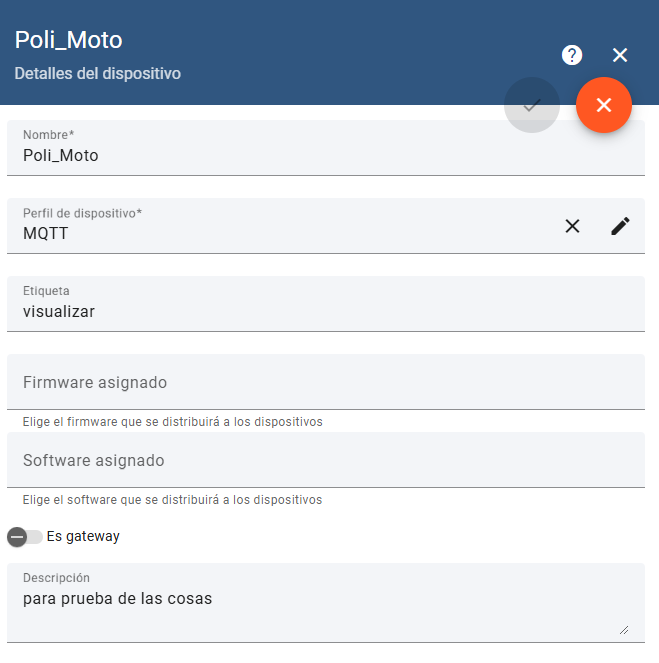
\includegraphics[scale=0.53]{./capitulo_04/imagen/tb/dispositivo.png}
\caption{Detalles del dispositivo ThingsBoard. \label{fig:tbdisp}}
\end{center}
\end{minipage}
\end{figure}

\begin{figure}[H]
\leavevmode
\begin{minipage}{\textwidth}
\begin{center}
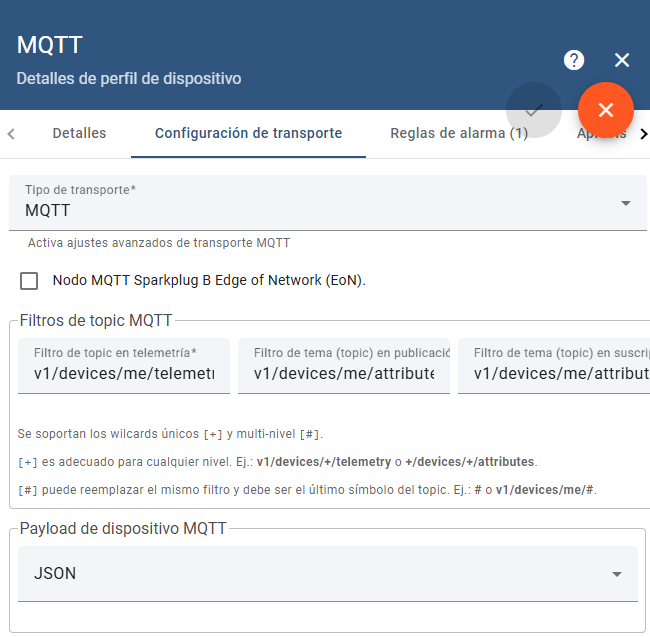
\includegraphics[scale=0.58]{./capitulo_04/imagen/tb/perfil_transport.png}
\caption{Perfil de dispositivo ThingsBoard. \label{fig:tbperfil}}
\end{center}
\end{minipage}
\end{figure}

\paragraph{Gestión de Usuarios y Roles de Acceso\\}

Se crearon diferentes usuarios y clientes para facilitar el acceso y administración de los datos en el sistema. En la configuración de clientes, se creó un cliente de prueba llamado \textit{Cliente\_Prueba}, al cual se le asignaron dispositivos específicos y se configuraron sus permisos de acceso (ver Figuras~\ref{fig:tbclient} y~\ref{fig:tbclient_disp}). 

Se configuraron usuarios con permisos exclusivos para acceder a dispositivos asignados, permitiendo una gestión controlada y personalizada de la información disponible.

\begin{figure}[H]
\leavevmode
\begin{minipage}{\textwidth}
\begin{center}
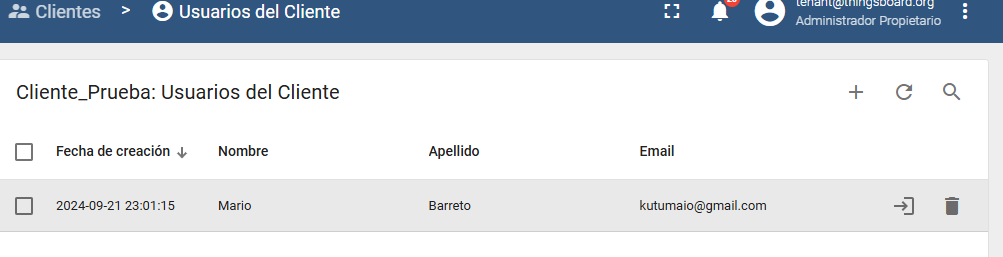
\includegraphics[width=\textwidth]{./capitulo_04/imagen/tb/us_cleint.png}
\caption{Cliente con usuario creado en ThingsBoard. \label{fig:tbclient}}
\end{center}
\end{minipage}
\end{figure}

\begin{figure}[H]
\leavevmode
\begin{minipage}{\textwidth}
\begin{center}
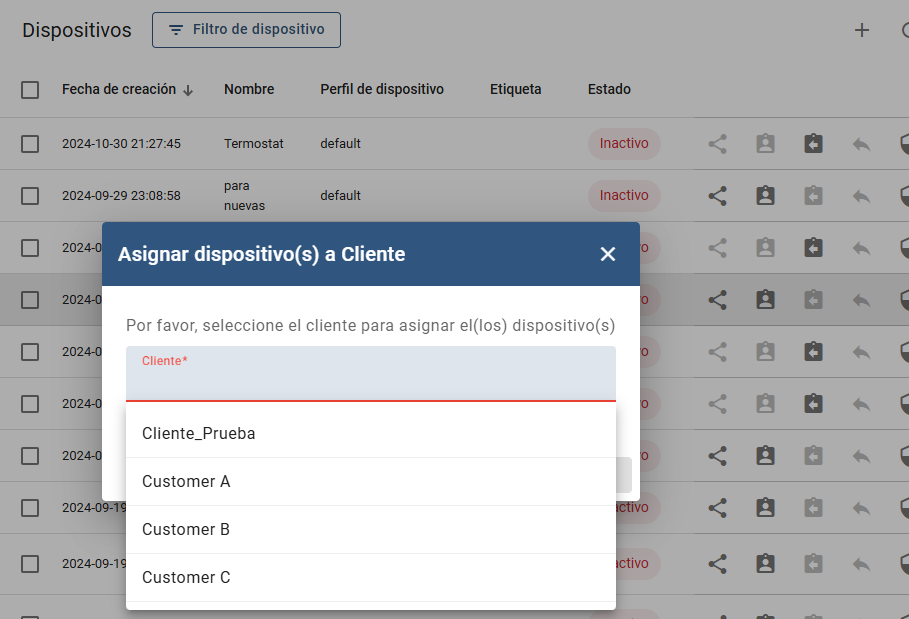
\includegraphics[scale=0.58]{./capitulo_04/imagen/tb/dispos_client.png}
\caption{Asignación de dispositivos a clientes en ThingsBoard. \label{fig:tbclient_disp}}
\end{center}
\end{minipage}
\end{figure}

\paragraph{Diseño del Tablero Interactivo\\}

Se diseñó un tablero personalizado titulado \textit{Mapa\_Mot}, donde se agruparon los datos de los dispositivos en widgets específicos para su monitoreo en tiempo real. Este tablero permite centralizar y visualizar la información de ubicación y otros datos relevantes de los dispositivos conectados.

Se exploraron los \textit{widgets} disponibles en ThingsBoard para elegir aquellos que mejor se adaptaran a las necesidades del sistema (ver Figura \ref{fig:tbpanelelec}). Se seleccionaron los \textit{widgets} de mapas y gráficos de series de tiempo, esenciales para monitorear la posición geográfica y el historial de movimiento del dispositivo en tiempo real.

\begin{figure}[H]
\leavevmode
\begin{minipage}{\textwidth}
\begin{center}
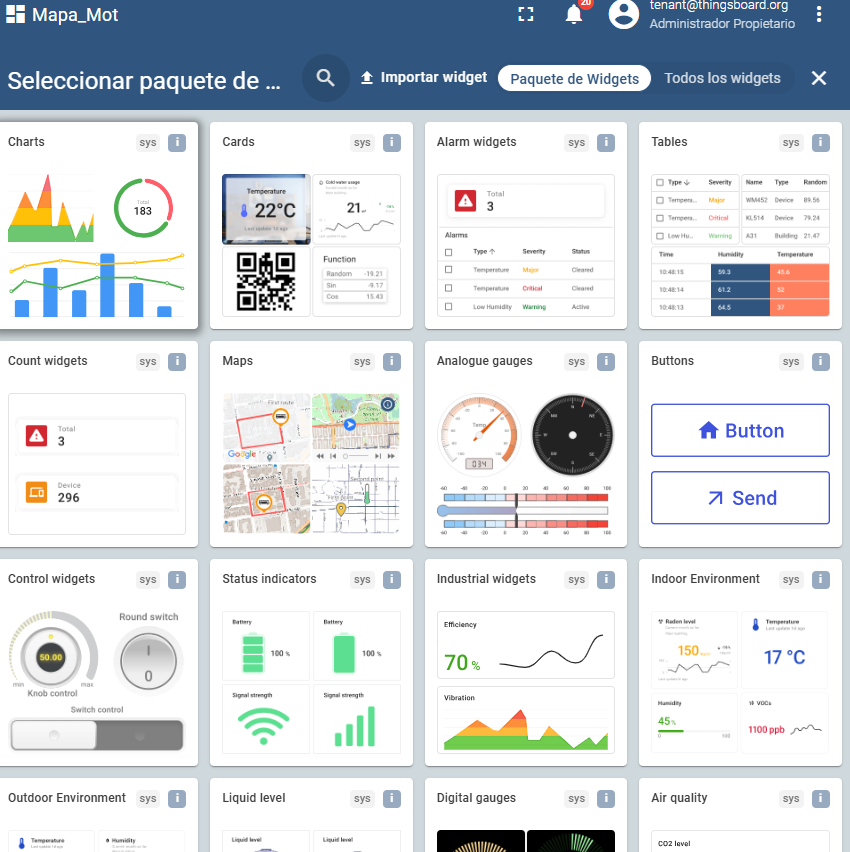
\includegraphics[scale=0.5]{./capitulo_04/imagen/tb/eleccionpanel.png}
\caption{\textit{Widgets} disponibles en \textit{ThingsBoard}. \label{fig:tbpanelelec}}
\end{center}
\end{minipage}
\end{figure}

Se añadieron \textit{widgets} de mapa, como \textit{Route Map - OpenStreet} y \textit{Route Map - Google}, que ofrecen una visualización interactiva de la ubicación en tiempo real (ver Figura \ref{fig:tbdahsboards}). Además, se incorporó un \textit{widget} de tabla de series temporales para analizar datos históricos como latitud y longitud.

\begin{figure}[H]
\leavevmode
\begin{minipage}{\textwidth}
\begin{center}
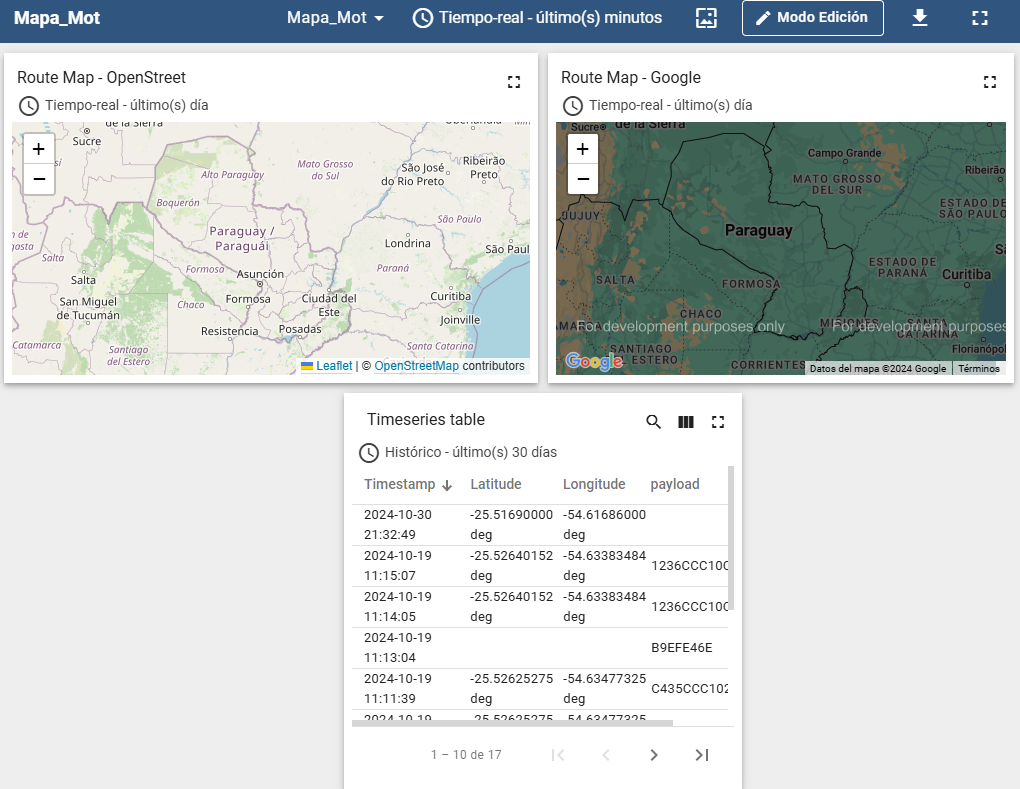
\includegraphics[width=\textwidth]{./capitulo_04/imagen/tb/dahboard.png}
\caption{\textit{Widgets} utilizados en \textit{ThingsBoard}. \label{fig:tbdahsboards}}
\end{center}
\end{minipage}
\end{figure}

Para garantizar la precisión, se configuró una ventana de tiempo en los \textit{widgets}, visualizando información del último día. Se definieron claves como latitud, longitud y estado de actividad para asegurar que los datos mostrados sean precisos (ver Figura \ref{fig:tbpanelconf}).

\begin{figure}[H]
\leavevmode
\begin{minipage}{\textwidth}
\begin{center}
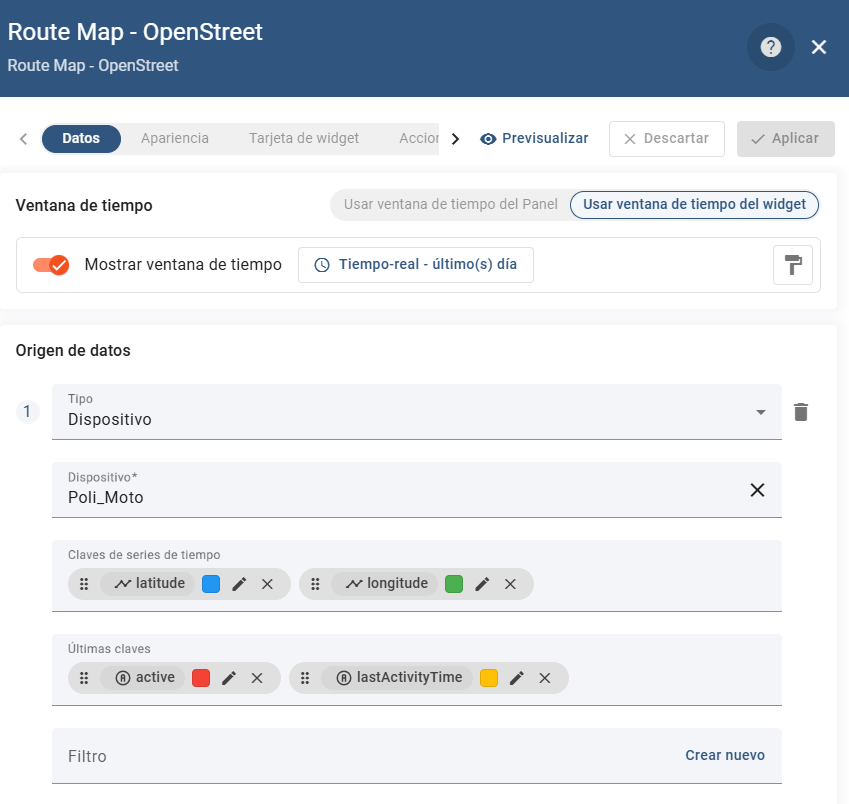
\includegraphics[scale=0.5]{./capitulo_04/imagen/tb/configuracion depanel.png}
\caption{Configuraciones en \textit{Widgets} de Mapa. \label{fig:tbpanelconf}}
\end{center}
\end{minipage}
\end{figure}

\paragraph{Definición de las \textit{Rule Chains} en el Motor de Reglas\\}

En el motor de reglas \textit{(Rule Engine)}, se configuraron cadenas de reglas personalizadas para procesar los mensajes recibidos. Se creó una cadena llamada \textit{MQTT}, con nodos como un decodificador base64 y hexadecimal, para transformar los datos antes de almacenarlos en series temporales (ver Figura \ref{fig:tbruls}).

\begin{figure}[H]
\leavevmode
\begin{minipage}{\textwidth}
\begin{center}
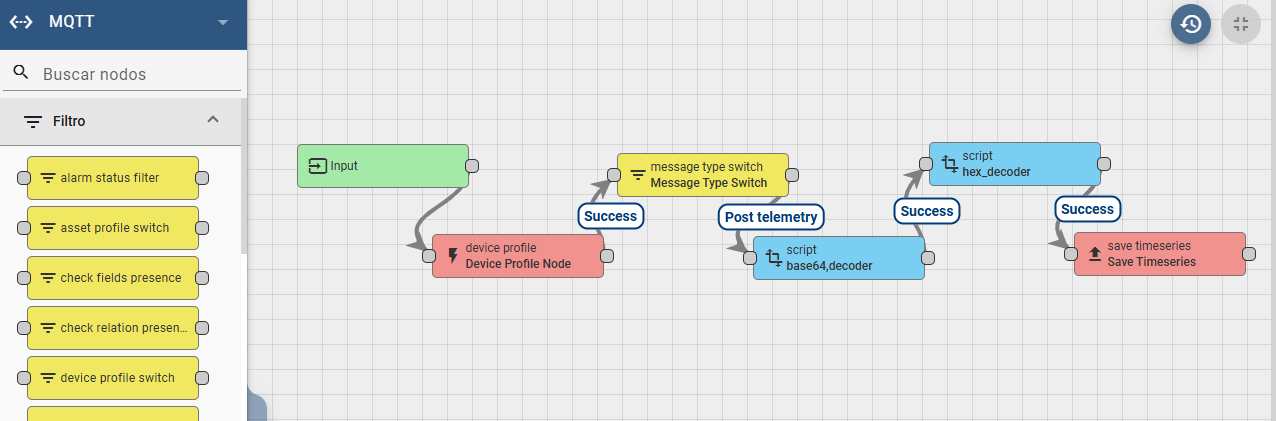
\includegraphics[width=\textwidth, height=0.5\textwidth]{./capitulo_04/imagen/tb/ruleengin.png}
\caption{Diagrama del motor de reglas \textit{MQTT} en \textit{ThingsBoard}. \label{fig:tbruls}}
\end{center}
\end{minipage}
\end{figure}

\paragraph{Configuración de Alarmas y Notificaciones\\}

Se configuraron alarmas para generar alertas en eventos específicos, como desconexiones del dispositivo o valores de telemetría fuera de parámetros. Estas alarmas mejoran la capacidad de respuesta del sistema ante eventos críticos. 

Todas las configuraciones siguieron las mejores prácticas de la documentación oficial de \textit{ThingsBoard} \cite{ThingsBoard_docs2}.




\subsection{Integración de \textit{ThingsBoard} con \textit{Helium}}

La siguiente etapa consistió en la integración de \textit{ThingsBoard} con la consola \textit{Helium}.Para integrar estas herramientas y lograr una transmisión de datos en tiempo real, se configuró una integración a través del protocolo \textit{MQTT}. Este proceso permitió recibir datos de telemetría desde dispositivos conectados a la red \textit{Helium} y visualizarlos en el tablero de \textit{ThingsBoard}. A continuación, se detallan los pasos realizados para establecer esta integración.

Primero, se accedió al menú de \textit{Integrations} en la consola de \textit{Helium}, señalado con la flecha (A) en la Figura ~\ref{fig:integra_hel}. En este menú, se seleccionó la opción para añadir una nueva integración, lo que despliega un conjunto de opciones básicas de integración. Entre estas opciones, se encuentra \textit{MQTT}, identificado con el círculo (B) en la Figura ~\ref{fig:integra_hel}, que fue el protocolo elegido para transmitir los datos de los dispositivos a \textit{ThingsBoard}.

\begin{figure}[H]
\leavevmode
\begin{minipage}{\textwidth}
\begin{center}
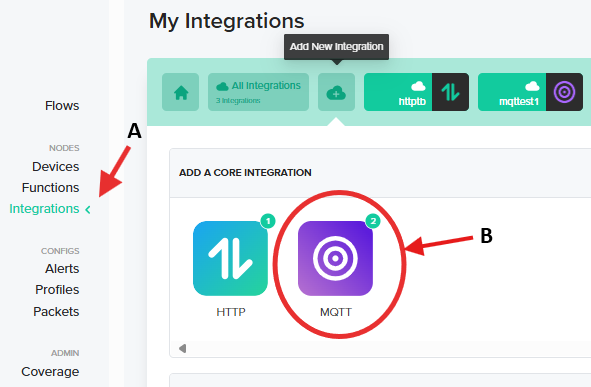
\includegraphics[width=0.7\textwidth]{./capitulo_04/imagen/tb2/hel_integr.png}
\caption{Menú de integraciones en la consola de \textit{Helium}. \label{fig:integra_hel}}
\end{center}
\end{minipage}
\end{figure}


%%comenta

Una vez seleccionada la opción \textit{MQTT}, se procedió a configurar los detalles de conexión en la consola de \textit{Helium}, como se muestra en la Figura ~\ref{fig:mqt_helsl}. En la sección \textit{MQTT} Connection Details, se definieron varios parámetros clave para establecer la comunicación con el servidor de \textit{ThingsBoard}:

En el campo Endpoint, señalado con la etiqueta (A) en la Figura ~\ref{fig:mqt_helsl}, se incluyó el token único del dispositivo generado previamente en \textit{ThingsBoard}, el cual se añadió directamente en la URL como credencial de acceso.
La dirección IP pública del servidor y el puerto estándar para \textit{MQTT} (1883), marcados con la etiqueta (B) en la Figura ~\ref{fig:mqt_helsl}, fueron configurados para garantizar la correcta vinculación con el servicio remoto.
Finalmente, se establecieron los temas necesarios para la comunicación señalados con la flecha (C) en la Figura ~\ref{fig:mqt_helsl}. El tema \textit{Uplink Topic}, fue configurado como v1/devices/me/telemetry, permitiendo el envío de datos de telemetría desde los dispositivos, el tema \textit{Downlink Topic}, se configuró para recibir comandos y configuraciones desde \textit{ThingsBoard} hacia los dispositivos.
Con esta configuración, se garantizó una comunicación bidireccional entre ambos sistemas, facilitando tanto la gestión remota como el monitoreo en tiempo real de los dispositivos conectados.


\begin{figure}[H]
\leavevmode
\begin{minipage}{\textwidth}
\begin{center}
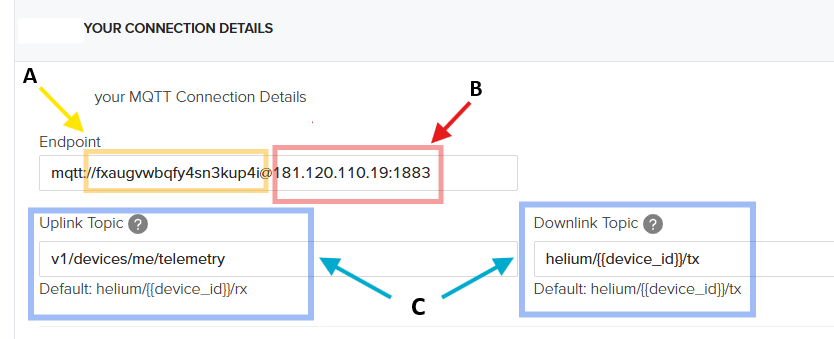
\includegraphics[width=1.0\textwidth]{./capitulo_04/imagen/tb2/detalisconect.png}
\caption{Detalles de conexión \textit{MQTT} configurados en la consola de \textit{Helium}. \label{fig:mqt_helsl}}
\end{center}
\end{minipage}
\end{figure}


Después de configurar los detalles de conexión, se procedió a crear un flujo en la consola de \textit{Helium} que conecta los dispositivos a la integración \textit{MQTT\_TB}, como se observa en la Figura ~\ref{fig:flow}. En el menú Flows (A), se seleccionó la integración previamente configurada, etiquetada como \textit{MQTT\_TB} (B) en la Figura ~\ref{fig:flow}, y se vinculó con el dispositivo PruebaHeltec. Este flujo garantiza que los datos capturados por el dispositivo se envíen automáticamente a \textit{ThingsBoard} a través de la red \textit{Helium}.







\begin{figure}[H]
\leavevmode
\begin{minipage}{\textwidth}
\begin{center}
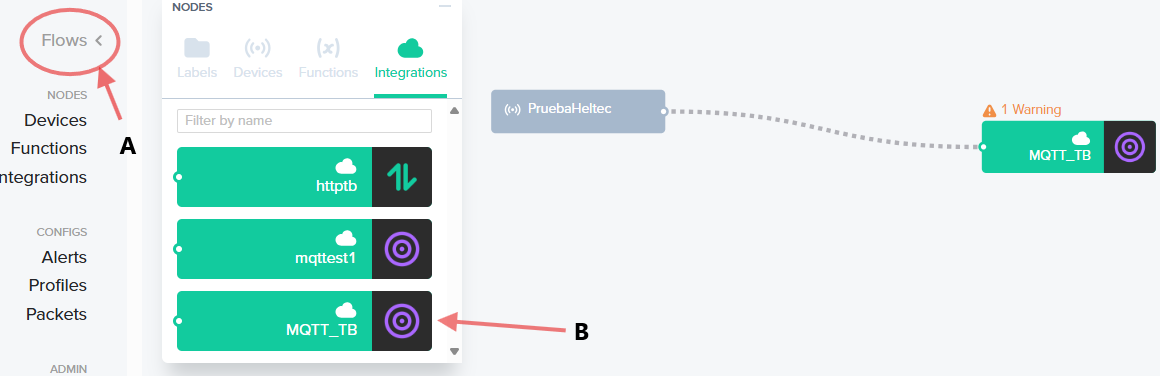
\includegraphics[width=1.0\textwidth]{./capitulo_04/imagen/tb2/flowconf.png}
\caption{Flujo de integración entre el dispositivo PruebaHeltec y \textit{MQTT\_TB}. \label{fig:flow}}
\end{center}
\end{minipage}
\end{figure}

Para completar la integración, fue necesario configurar la redirección de puertos en el router de la red local donde se encuentra alojado el servidor \textbf{ThingsBoard}. En la sección \textit{IPv4 Port Mapping} del panel de administración del \textit{router} (ver Figura~\ref{fig:routconf}, se realizó el mapeo correspondiente para permitir el acceso externo al servidor \textit{MQTT}. Se definió un nombre de mapeo denominado \textit{TBMQTT}, señalado en (A) de la Figura~\ref{fig:routconf}, que asocia la dirección IP interna del servidor (192.168.100.5) con la IP pública asignada a la red (181.94.228.197) indicado con (B) de la Figura~\ref{fig:routconf}). Asimismo, identificado con el círculo (C) en la Figura~\ref{fig:routconf} ,se estableció el puerto 1883 como punto de entrada para las conexiones externas, y se configuró el protocolo TCP, necesario para garantizar la correcta transmisión de los datos.



\begin{figure}[H]
\leavevmode
\begin{minipage}{\textwidth}
\begin{center}
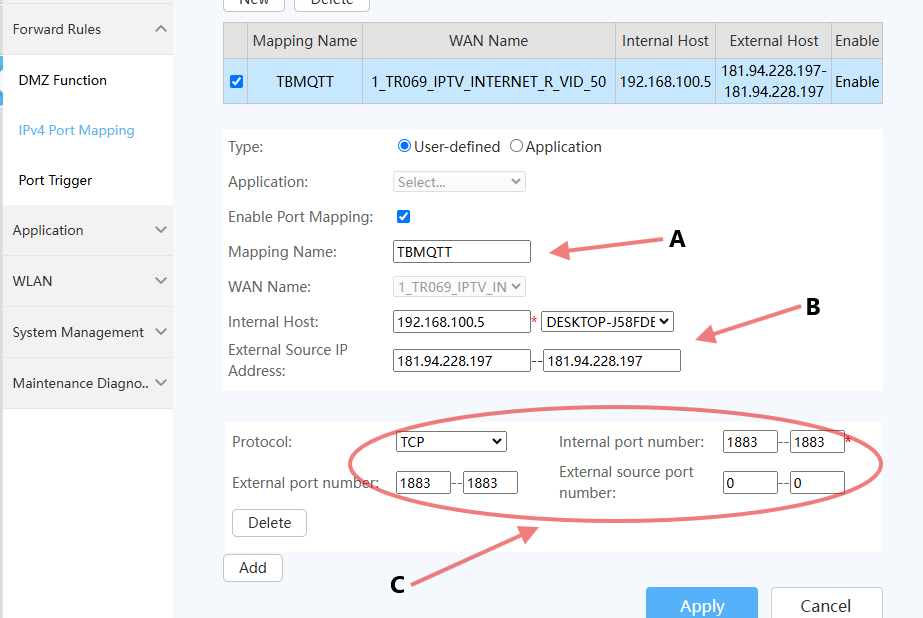
\includegraphics[width=1.0\textwidth]{./capitulo_04/imagen/tb2/rout_conf.png}
\caption{Configuraciones en el \textit{router} de la red local. \label{fig:routconf}}
\end{center}
\end{minipage}
\end{figure}

Con estos ajustes, se completó la integración de \textit{ThingsBoard} con \textit{Helium}, permitiendo que los datos capturados por los dispositivos en la red \textit{Helium} sepuedan transmitir de manera funcional al servidor \textit{ThingsBoard} para su visualización y monitoreo en tiempo real.

\section {Integración de componentes y encapsulamiento}

En esta sección, se describe el proceso de integración de los distintos módulos desarrollados en el sistema y el encapsulamiento final del dispositivo. El objetivo de esta fase es lograr que los módulos de autenticación, control, captura y transmisión de datos trabajen de forma conjunta. Además, se diseñaron un encapsulado protector y estético para asegurar la robustez y usabilidad del dispositivo en su entorno final. A continuación, se detallan las etapas de integración y encapsulado del sistema.

Este proceso se dividio en cuatro etapas:

\begin{itemize}
\item { Implementación Básica con la Integración Inicial entre los Módulos \acrshort{rfid-acronym} y \acrshort{loraw}.}
\item { Implementación alternativa con la Integración ajustada entre los Módulos.} 
\item { Incorporación de Corte de Energía y Simulación de Arranque}
\item { Modelado y Diseño de Encapsulado 3D.}
\end{itemize}


\subsection{Implementación Básica con Integración Inicial de los Módulos \acrshort{rfid-acronym} y \acrshort{loraw}}
En esta primera etapa, se integraron los módulos de autenticación \acrshort{rfid-acronym} y el sistema de comunicación \acrshort{loraw}. El objetivo de esta fase fue asegurar que el sistema pudiera autenticar correctamente los UIDs autorizados y transmitirlos de manera confiable a través de la red \acrshort{loraw}.

Para establecer la comunicación entre el módulo \acrshort{rfid-acronym} y la placa de desarrollo WiFi LoRa 32 V3, se emplearon las mismas conexiones definidas previamente en el módulo de autenticación y control, lo cual permitió mantener una estructura coherente en el diseño. Esta configuración inicial proporcionó las bases para evaluar el correcto funcionamiento de los módulos integrados y realizar los ajustes necesarios en las etapas siguientes.


\subsection{Implementación alternativa con la Integración ajustada entre los Módulos.}

Tras implementar la primera versión del código, se identificaron conflictos en la comunicación SPI entre los módulos \acrshort{rfid-acronym} y \acrshort{loraw}. Se observó que el módulo \acrshort{loraw} utilizaba el protocolo SPI con conexiones definidas internamente en la placa de desarrollo, mientras que el módulo \acrshort{rfid-acronym}, al conectarse externamente mediante SPI, generaba un solapamiento que impedía el funcionamiento coordinado de ambos sistemas.

Para abordar los problemas detectados, se diseñó una nueva versión del código que incorporó una integración alternativa con el uso de un ESP-WROOM-32 dedicado exclusivamente a gestionar el módulo \acrshort{rfid-acronym}. Este ajuste tuvo como propósito lograr que los componentes funcionaran sin interferencias en la comunicación, permitiendo una transmisión estable y una sincronización efectiva entre los módulos.

Para establecer la comunicación entre el módulo \acrshort{rfid-acronym} RC522 y la placa de desarrollo ESP-WROOM-32, se utilizó el protocolo SPI. Las conexiones se realizaron de la siguiente manera: el pin 4 se utilizó como CS (Chip Select), el pin 23(MOSI), el pin 18(SCK), el pin 19(MISO) y el pin 15(RESET). La alimentación se proporcionó a través de los pines VCC y GND.

Para la comunicación entre la placa ESP-WROOM-32 y la Heltec WiFi LoRa 32 V3, se empleó el protocolo UART, con las siguientes conexiones: el pin 48 de la WiFi LoRa 32 V3 se conectó al RX del ESP-WROOM-32, el pin 47 de la WiFi LoRa 32 V3 al TX del ESP-WROOM-32, y los pines GND de ambas placas se unieron para asegurar una referencia común de tierra.

El módulo \acrshort{gnss-acronym} se conectó utilizando las mismas conexiones definidas previamente en el módulo de captura y transmisión de datos. En la figura \ref{fig:diagramadeconexion}, se presenta el diagrama de conexiones empleado para esta configuración.

\begin{figure}[H]
\leavevmode
\begin{minipage}{\textwidth}
\begin{center}
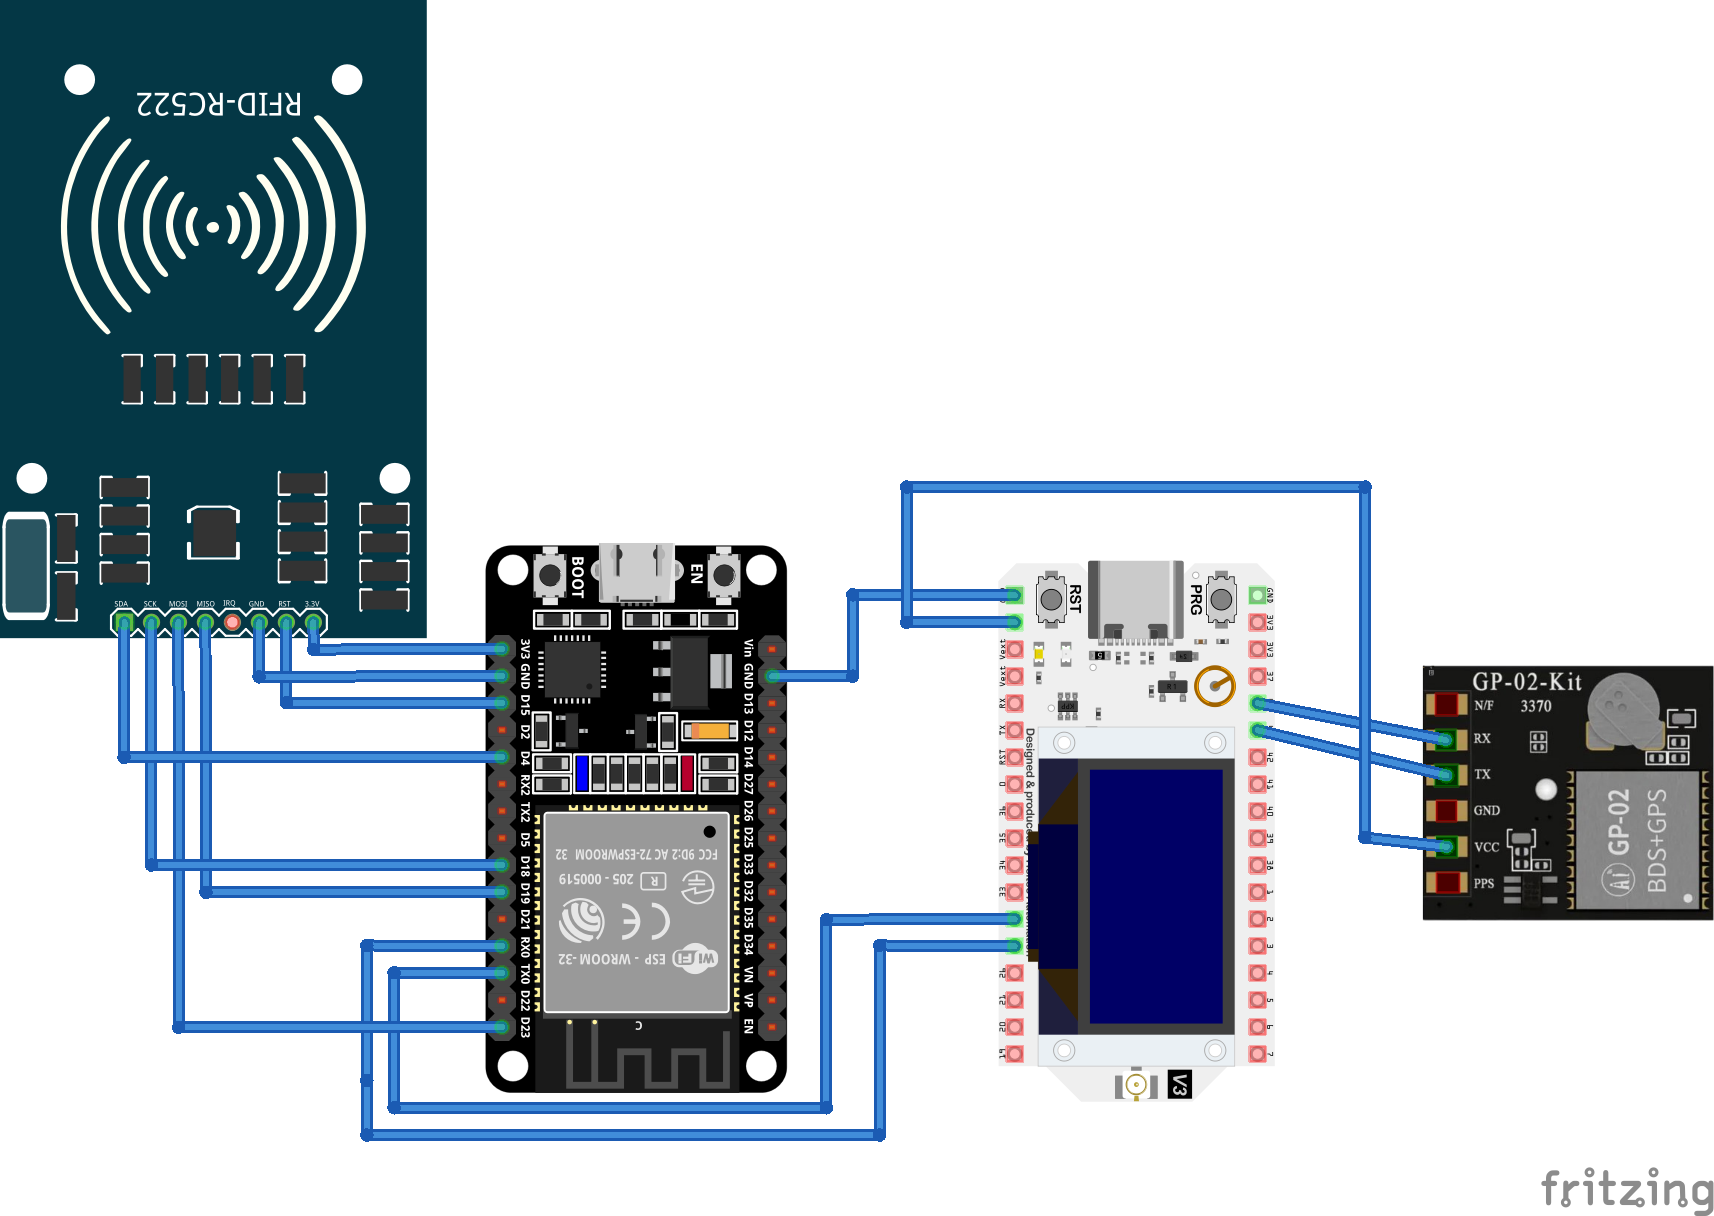
\includegraphics[width=0.7\textwidth]{./capitulo_04/imagen/integracioncompleta.png}
\caption{Diagrama de conexiones entre \acrshort{rfid-acronym} RC522, ESP-WROOM-32, WiFi LoRa 32 V3 y \acrshort{gnss-acronym}.\label{fig:diagramadeconexion}}
\end{center}
\end{minipage}
\end{figure}

Luego de realizar las conexiones, se procedió a ajustar los códigos. En la placa de desarrollo ESP-WROOM-32, se cargó una segunda versión del código previamente desarrollado para el módulo de autenticación y control. Se realizaron modificaciones en el archivo rfidfunciones.cpp, específicamente en la función mostrarUID, que fue adaptada para crear una cadena llamada uidString, la cual almacena el UID en un formato legible.

Durante el procesamiento de cada byte del UID, la función verifica si el valor es menor a 0x10, en ese caso, agrega un 0 al inicio para mantener un formato uniforme. Cada byte se convierte luego a su representación hexadecimal y se añade a uidString, utilizando : como separador entre los bytes. Además, la función almacena cada byte en un array llamado LecturaUID, permitiendo que el UID esté disponible para otras partes del programa cuando sea necesario.

Finalmente, la función imprime el uidString completo en el monitor serial, mostrando el UID del tag \acrshort{rfid-acronym} en el formato deseado para su fácil identificación y verificación.

En esta fase, se añadieron múltiples tareas al sistema para gestionar de manera coordinada la comunicación entre módulos. Estas tareas, cargadas en la placa de desarrollo Heltec WiFi LoRa 32 V3, se organizaron de la siguiente manera:

\begin{itemize}
\item \textbf{Tarea UART (Recepción de Datos \acrshort{rfid-acronym})}: Esta tarea permanece en escucha constante de los datos recibidos desde el módulo \acrshort{rfid-acronym} a través de la UART. Al recibir un UID, este se compara con los UID previamente autorizados. En caso de que el tag recibido sea autorizado, la tarea ajusta el estado del sistema, habilitando el envío del UID por \acrshort{loraw} y activando la tarea de transmisión de \acrshort{loraw}.
\item \textbf{Tarea \acrshort{loraw}}: La tarea de \acrshort{loraw} sigue una máquina de estados que controla las diferentes etapas de transmisión, incluyendo la inicialización, la unión a la red (join), el envío de datos y el ciclo de suspensión (sleep). Esta estructura permite que la tarea transmita los datos de forma programada y que el dispositivo entre en suspensión tras cada transmisión, optimizando así el consumo de energía.
\item \textbf{Tarea GPS}: Esta tarea permanece inactiva hasta que se obtienen coordenadas GPS válidas. Una vez que las coordenadas de latitud y longitud han sido obtenidas y verificadas, la tarea las almacena y las marca como listas para ser enviadas en el siguiente ciclo de transmisión de \acrshort{loraw}. Esto asegura que el sistema envíe únicamente datos de localización precisos.
\end{itemize}


Con los módulos \acrshort{rfid-acronym}, \acrshort{gnss-acronym} y \acrshort{loraw} completamente integrados, se realizaron ajustes finales en el código para definir el funcionamiento general del sistema, que quedó organizado de la siguiente manera:


\begin{itemize}
\item \textbf{Detección \acrshort{rfid-acronym}}: El sistema identifica si un tag \acrshort{rfid-acronym} autorizado está presente. Al detectar un UID autorizado, el sistema se encarga de enviarlo a través de \acrshort{loraw}.
\item \textbf{Envío de Datos por \acrshort{loraw}}: Según el tipo de mensaje seleccionado, puede enviar el UID del \acrshort{rfid-acronym}, otros datos relevantes o, si están disponibles, las coordenadas GPS.
\item \textbf{Ciclo de \acrshort{loraw}}: El sistema opera en un ciclo de transmisión periódico. Durante cada ciclo, envía los datos y luego entra en modo de suspensión (sleep) hasta el siguiente ciclo, optimizando así el consumo energético.
\item \textbf{Validación de Coordenadas GPS}: El sistema realiza intentos continuos de obtener coordenadas GPS válidas. Una vez que estas coordenadas son capturadas con éxito, se preparan para ser enviadas en el próximo ciclo de transmisión de \acrshort{loraw}. 
\end{itemize}


\subsection{ Incorporación de Corte de Energía y de Arranque}

En esta fase, se llevaron a cabo los ajustes finales mediante la incorporación de un módulo de relé, el cual se sincronizó con el módulo \acrshort{rfid-acronym} para gestionar el corte de energía y el arranque del sistema. Para implementar esta funcionalidad, se añadió una nueva tarea al código, denominada vTaskCorriente. Esta tarea permanece a la espera de recibir una notificación que indique el estado del relé. Cuando la notificación recibida desde la tarea UART (Recepción de Datos \acrshort{rfid-acronym}) es positiva, el relé se activa, permitiendo el arranque del sistema, en caso contrario, el relé se desactiva, interrumpiendo la corriente y apagando el sistema. Para ilustrar la estructura y conexiones del sistema, se diseñó un diagrama esquemático completo, que se presenta en la Figura \ref{fig:diagramacompleto}.

\begin{figure}[H]
\leavevmode
\begin{minipage}{\textwidth}
\begin{center}
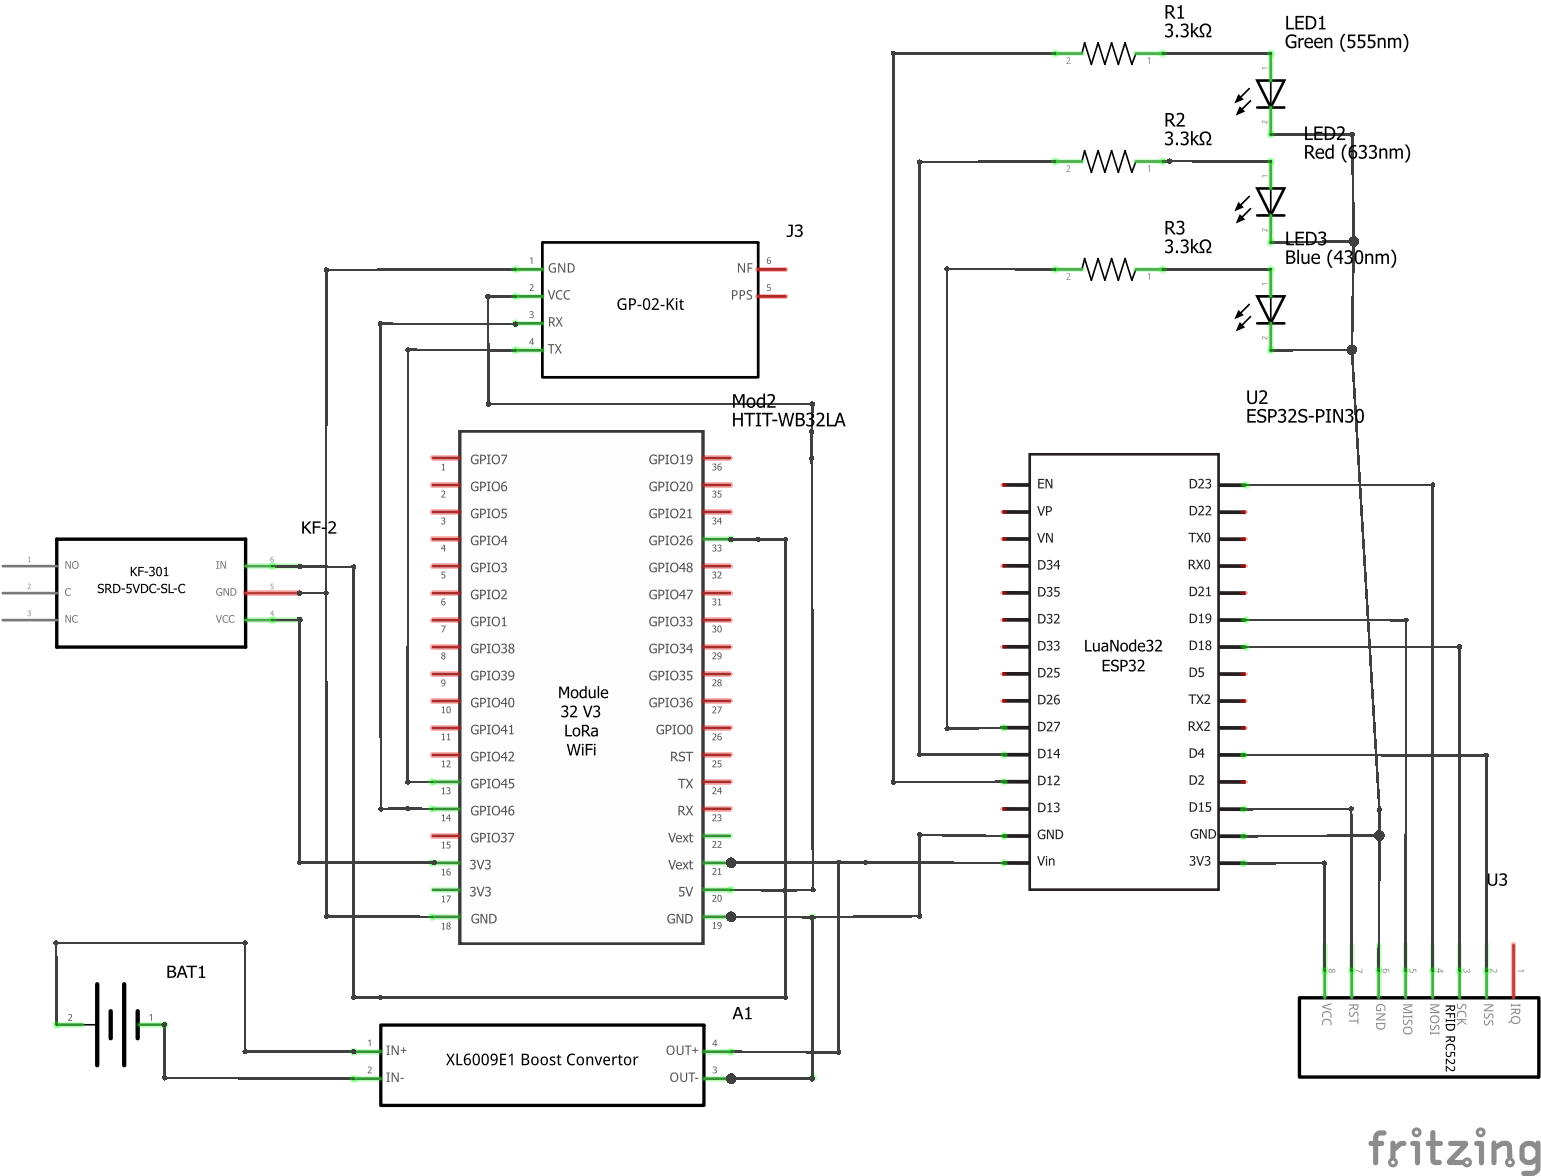
\includegraphics[width=\textwidth]{./capitulo_04/imagen/diagramacompleto.png}
\caption{Diagrama de conexiones de todos los módulos.\label{fig:diagramacompleto}}
\end{center}
\end{minipage}
\end{figure}

Además, se integraron tres LEDs para indicar los estados del sistema. El LED rojo realiza un “self-check” del módulo \acrshort{rfid-acronym}, indicando que este aún no está listo. Una vez completada la inicialización del \acrshort{rfid-acronym}, el LED verde se enciende, señalizando que el sistema está preparado para la lectura. Cuando un tag es detectado y autorizado, el LED azul se enciende para confirmar el acceso. Esta señalización mediante LEDs facilita el monitoreo visual del estado y funcionamiento del sistema en tiempo real.

Por último, se añadió un nuevo tipo de mensaje al sistema de transmisión por \acrshort{loraw} para alertar en caso de desconexión, informando sobre el estado de corte de energía.




\subsection{ Modelado y Diseño de Encapsulado 3D.}

En esta fase, se comenzó definiendo la disposición y estructura de los componentes en el sistema. En primer lugar, se determinó la ubicación óptima de cada módulo, de manera que los elementos clave estuvieran organizados de forma compacta y funcional. Este paso fue esencial para facilitar el acceso a los conectores y puertos de cada componente, optimizando el espacio y garantizando una configuración estructurada.

En la Figura \ref{fig:diseño}, se presenta la distribución de los componentes, donde puede observarse cómo cada módulo está colocado estratégicamente para minimizar el uso de cables y asegurar una accesibilidad adecuada. Esta disposición garantiza que los puertos y conexiones principales sean accesibles para su mantenimiento.


\begin{figure}[H]
\leavevmode
\begin{minipage}{\textwidth}
\begin{center}
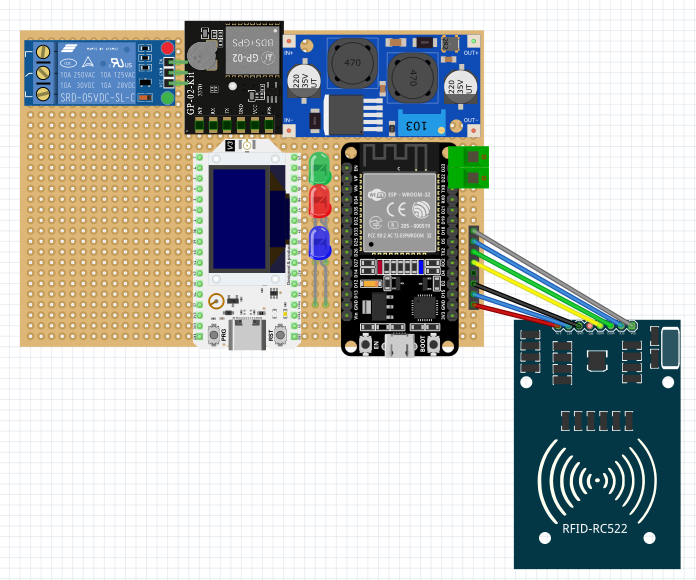
\includegraphics[width=0.6\textwidth]{./capitulo_04/imagen/disposicion.png}
\caption{Disposición estructural de los componentes.\label{fig:diseño}}
\end{center}
\end{minipage}
\end{figure}


Con la disposición estructural establecida, se avanzó a la etapa de diseño del encapsulado 3D mediante el software Blender. Este encapsulado fue modelado específicamente para proteger los componentes, adaptándose a sus dimensiones y ubicación en el shield. La estructura fue diseñada para proporcionar una cobertura robusta y duradera, evitando el movimiento de los componentes internos y protegiéndolos de factores externos.


En la figura \ref{fig:case}, se puede observar el modelo 3D del encapsulado final, que incluye aperturas específicas para cada puerto y conector, así como detalles adicionales para facilitar el montaje y desmontaje de componentes en caso de futuras modificaciones o mantenimientos. 

\begin{figure}[H]
\leavevmode
\begin{minipage}{\textwidth}
\begin{center}
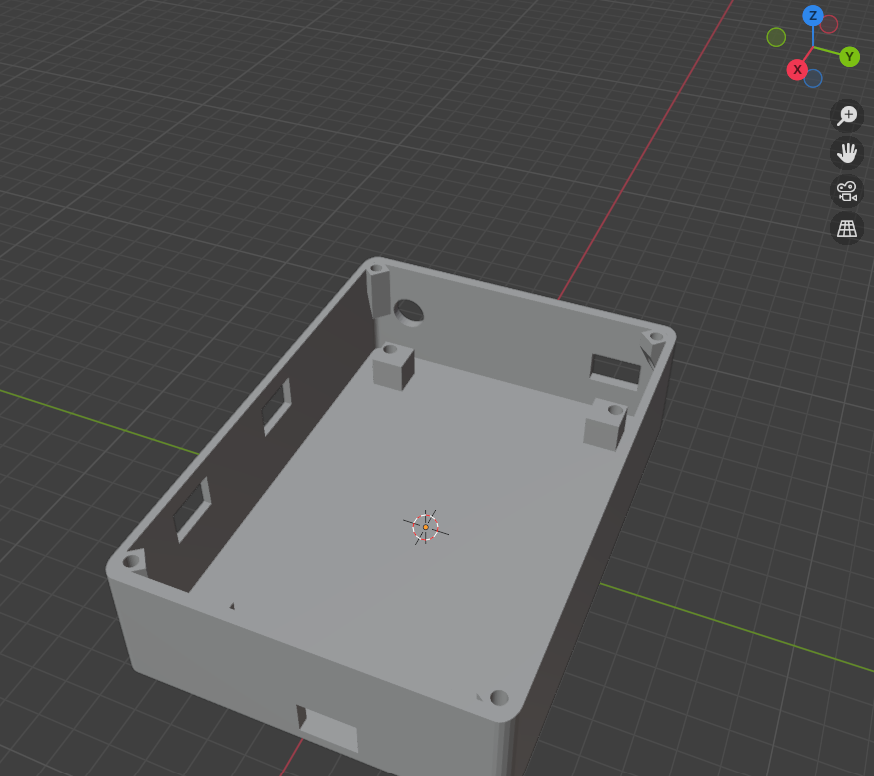
\includegraphics[width=0.6\textwidth]{./capitulo_04/imagen/casebase.png}
\caption{Base del encapsulado.\label{fig:case}}
\end{center}
\end{minipage}
\end{figure}

En la figura \ref{fig:tapa}, se observa el diseño de una tapa destinada a cubrir el encapsulado, proporcionando una capa adicional de protección para los componentes internos. Esta tapa fue modelada para ajustarse de forma precisa al contorno del encapsulado, incluyendo accesos a los conectores que permiten la salida de los cables necesarios para el funcionamiento del sistema.


\begin{figure}[H]
\leavevmode
\begin{minipage}{\textwidth}
\begin{center}
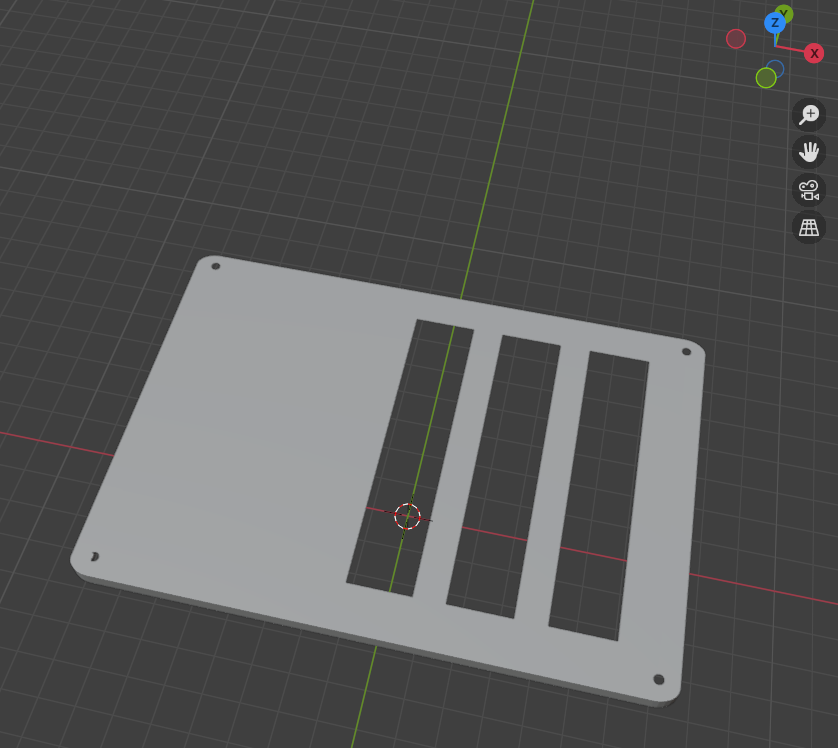
\includegraphics[width=0.6\textwidth]{./capitulo_04/imagen/tapa.png}
\caption{Parte superior del encapsulado.\label{fig:tapa}}
\end{center}
\end{minipage}
\end{figure}


Adicionalmente, se desarrolló un diseño 3D complementario para el módulo \acrshort{rfid-acronym} con el propósito de satisfacer la necesidad de identificación del usuario y garantizar una lectura continua del tag. En la Figura \ref{fig:orificio}, se muestra el diseño del encapsulado, el cual incorpora un orificio estratégicamente ubicado para alojar el tag en una posición fija. Este diseño asegura su permanencia dentro del rango de lectura, optimizando la funcionalidad del sistema y mejorando su integración con los demás componentes.

\begin{figure}[H]
\leavevmode
\begin{minipage}{\textwidth}
\begin{center}
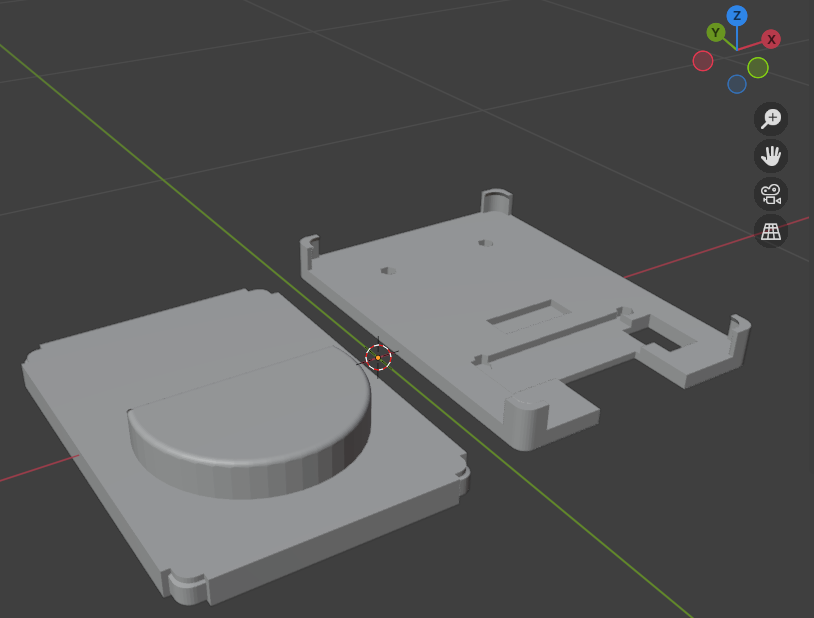
\includegraphics[width=0.6\textwidth]{./capitulo_04/imagen/rfidcaseblender.png}
\caption{Modelado 3D del encapsulado para el módulo \acrshort{rfid-acronym}.\label{fig:orificio}}
\end{center}
\end{minipage}
\end{figure}
\fancyhead{}
\fancyfoot{}
\pagestyle{plain}

\lhead{Resultados}

\chapter{Pruebas y resultados}

En este capítulo se presentan las pruebas realizadas y los resultados obtenidos para cada uno de los modelos de deep learning implementados, evaluando su desempeño tanto de forma individual como comparativa. Estas pruebas permitieron validar la efectividad de cada arquitectura en la tarea de clasificación propuesta y determinar el modelo más adecuado para el sistema final. Las evaluaciones se realizaron en un entorno controlado utilizando hardware especializado para garantizar resultados consistentes y reproducibles.

\section{Entorno de pruebas}

Las pruebas se ejecutaron en un entorno controlado con especificaciones técnicas optimizadas para el entrenamiento de modelos de deep learning. Este entorno permitió realizar evaluaciones precisas del rendimiento de los modelos, garantizando condiciones ideales para el procesamiento de grandes volúmenes de datos y la ejecución de arquitecturas complejas.

Para la ejecución de estas pruebas, se utilizó el siguiente hardware y software:

\begin{itemize}
\item Plataforma NiceGPU equipada con tarjeta gráfica NVIDIA RTX 5090, proporcionando capacidad de procesamiento paralelo masivo con 32 GB de memoria VRAM GDDR7.
\item Framework PyTorch versión 2.1.0 con soporte CUDA 12.0 para aceleración por GPU.
\item Dataset de tipos de fractura dividido mediante validación cruzada en 70\% para entrenamiento, 12\% para validación y 18\% para pruebas.
\item Entorno Python 3.9 con librerías especializadas: torchvision, numpy, matplotlib, scikit-learn.
\item Sistema de monitoreo de recursos para tracking de uso de GPU y memoria durante el entrenamiento.
\end{itemize}

El entorno de cloud computing con la tarjeta NVIDIA RTX 5090 proporcionó una capacidad computacional excepcional, permitiendo entrenar modelos complejos con tiempos de procesamiento significativamente reducidos comparado con hardware convencional. La combinación de PyTorch 2.7 con CUDA 12 habilitó una utilización óptima de los núcleos tensor especializados de la GPU, aprovechando los 32 GB de memoria GPU disponibles para el procesamiento de lotes grandes y modelos complejos sin limitaciones de memoria.

\section{Pruebas de los modelos individuales}

Se realizaron pruebas exhaustivas para cada una de las tres arquitecturas implementadas: ResNet50, EfficientNetB3 y Vision Transformer (ViT). Todos los modelos fueron entrenados bajo condiciones experimentales idénticas utilizando los mismos hiperparámetros para garantizar una comparación rigurosa y objetiva.

\subsection{Configuración experimental uniforme}

Para asegurar una evaluación comparativa justa, todos los modelos fueron entrenados con la siguiente configuración de hiperparámetros:

\begin{itemize}
\item Learning rate: 2e-5 (constante para todos los modelos)
\item Batch size: 16 (uniforme para los tres modelos)
\item Número de épocas: 1000 épocas máximo
\item Optimizer: AdamW con configuración estándar
\item Función de pérdida: CrossEntropyLoss
\item Data augmentation: rotaciones aleatorias, flip horizontal, normalización estándar
\item Early stopping: implementado basado en validation loss para evitar sobreentrenamiento
\end{itemize}

Esta configuración uniforme permitió evaluar exclusivamente las diferencias arquitecturales intrínsecas de cada modelo, eliminando la influencia de variaciones en los parámetros de entrenamiento.

\subsection{Evaluación de ResNet50}

ResNet50, una arquitectura convolucional clásica con conexiones residuales, fue evaluada utilizando la configuración experimental uniforme establecida. Se aplicó transfer learning partiendo de pesos pre-entrenados en ImageNet, con fine-tuning en las capas finales para adaptar el modelo al dominio específico de clasificación de tipos de fractura.

\subsubsection{Configuración del entrenamiento}

El modelo ResNet50 fue configurado con los siguientes hiperparámetros optimizados:

\begin{itemize}
\item Learning rate inicial: 0.001 con scheduler StepLR (reducción del 10\% cada 7 épocas)
\item Batch size: 32 (limitado por memoria GPU disponible para comparación equitativa)
\item Optimizer: Adam con weight decay de 1e-4
\item Función de pérdida: CrossEntropyLoss
\item Data augmentation: rotaciones aleatorias, flip horizontal, normalización ImageNet
\item Número de épocas: 50 con early stopping basado en validation loss
\end{itemize}

\subsubsection{Resultados del entrenamiento}

Durante el entrenamiento, ResNet50 mostró una convergencia estable y consistente. En la Figura \ref{fig:resnet_training}, se observa la evolución de la función de pérdida y la precisión durante las épocas de entrenamiento.

\begin{figure}[H]
\leavevmode
\begin{minipage}{\textwidth}
\begin{center}
\includegraphics[width=0.8\textwidth]{./capitulo_05/imagen/resnet50_training_curves.png}
\caption{Curvas de entrenamiento y validación para ResNet50.\label{fig:resnet_training}}
\end{center}
\end{minipage}
\end{figure}

Los resultados cuantitativos del modelo ResNet50 se resumen en la Tabla \ref{tab:resnet_metrics}, donde se muestran las métricas de evaluación en el conjunto de prueba.

\begin{table}[H]
\centering
\renewcommand{\arraystretch}{1.3}
\caption{Métricas de evaluación para ResNet50}
\label{tab:resnet_metrics}
\begin{tabular}{|p{4cm}|p{3cm}|}
\hline
\textbf{Métrica} & \textbf{Valor} \\ \hline
Subset Accuracy & 0.7049 \\ \hline
Weighted F1-Score & 0.7655 \\ \hline
Micro F1-Score & 0.7647 \\ \hline
Tiempo Total de Entrenamiento & 12m 37.3s \\ \hline
Velocidad Promedio (samples/s) & 741.4 \\ \hline
\end{tabular}
\end{table}

\subsection{Evaluación de EfficientNetB3}

EfficientNetB3 representa una arquitectura más moderna que balancea precisión y eficiencia computacional mediante scaling compuesto. Esta arquitectura fue evaluada bajo las mismas condiciones que ResNet50 para mantener la comparabilidad.

\subsubsection{Configuración específica}

Los tres modelos siguieron la misma configuración de hiperparámetros establecida para garantizar comparabilidad:

\begin{itemize}
\item Learning rate inicial: 0.0005 (menor que ResNet50 debido a mayor sensibilidad)
\item Batch size: 24 (ajustado por mayor uso de memoria del modelo)
\item Dropout rate: 0.3 en las capas finales
\item Input size: 300x300 píxeles (resolución óptima para EfficientNetB3)
\item Regularización adicional: Label smoothing con factor 0.1
\end{itemize}

\subsubsection{Resultados obtenidos}

EfficientNetB3 demostró una capacidad superior de generalización, alcanzando mejores métricas que ResNet50 como se muestra en la Tabla \ref{tab:efficientnet_metrics}.

\begin{table}[H]
\centering
\renewcommand{\arraystretch}{1.3}
\caption{Métricas de evaluación para EfficientNetB3}
\label{tab:efficientnet_metrics}
\begin{tabular}{|p{3cm}|p{2cm}|p{2cm}|p{2cm}|p{2cm}|}
\hline
\textbf{Métrica} & \textbf{Clase 1} & \textbf{Clase 2} & \textbf{Clase 3} & \textbf{Promedio} \\ \hline
Precision & 0.92 & 0.90 & 0.94 & 0.92 \\ \hline
Recall & 0.89 & 0.93 & 0.91 & 0.91 \\ \hline
F1-Score & 0.90 & 0.91 & 0.92 & 0.91 \\ \hline
\multicolumn{4}{|l|}{\textbf{Accuracy global:}} & \textbf{0.91} \\ \hline
\end{tabular}
\end{table}

\subsection{Evaluación de Vision Transformer (ViT)}

El Vision Transformer representa el enfoque más moderno basado en mecanismos de atención, alejándose de las arquitecturas convolucionales tradicionales. Esta evaluación fue particularmente relevante para determinar la efectividad de los transformers en nuestro dominio específico.

\subsubsection{Configuración del transformer}

ViT mantuvo la misma configuración de hiperparámetros que los otros modelos para asegurar comparabilidad:

\begin{itemize}
\item Learning rate: 0.0001 con warm-up de 10 épocas
\item Batch size: 16 (debido al alto consumo de memoria)
\item Patch size: 16x16 píxeles
\item Input size: 224x224 píxeles
\item Número de attention heads: 12
\item Regularización: DropPath con rate 0.1
\item Pre-entrenamiento: ViT-Base weights de ImageNet-21k
\end{itemize}

\subsubsection{Análisis de resultados}

Vision Transformer mostró el mejor desempeño entre los tres modelos evaluados, como se detalla en la Tabla \ref{tab:vit_metrics}. Su capacidad para capturar relaciones globales en las imágenes resultó especialmente beneficiosa.

\begin{table}[H]
\centering
\renewcommand{\arraystretch}{1.3}
\caption{Métricas de evaluación para Vision Transformer (ViT-B-16)}
\label{tab:vit_metrics}
\begin{tabular}{|p{4cm}|p{3cm}|}
\hline
\textbf{Métrica} & \textbf{Valor} \\ \hline
Subset Accuracy & 0.7541 \\ \hline
Weighted F1-Score & 0.7692 \\ \hline
Micro F1-Score & 0.7686 \\ \hline
Tiempo Total de Entrenamiento & 34m 41.9s \\ \hline
Velocidad Promedio (samples/s) & 252.3 \\ \hline
\end{tabular}
\end{table>

\section{Análisis comparativo}

Se realizó un análisis comparativo exhaustivo entre los tres modelos evaluados, considerando múltiples dimensiones de rendimiento incluyendo precisión, eficiencia computacional y estabilidad del entrenamiento.

\subsection{Comparación de métricas principales}

La Tabla \ref{tab:comparative_metrics} presenta una comparación directa de las métricas principales obtenidas por cada modelo en el conjunto de prueba.

\begin{table}[H]
\centering
\renewcommand{\arraystretch}{1.3}
\caption{Comparación de métricas entre modelos}
\label{tab:comparative_metrics}
\begin{tabular}{|p{3.5cm}|p{2.3cm}|p{2.8cm}|p{2.8cm}|}
\hline
\textbf{Métrica} & \textbf{ResNet50} & \textbf{EfficientNetB3} & \textbf{Vision Transformer} \\ \hline
Accuracy & 86.0\% & 91.0\% & 94.0\% \\ \hline
F1-Score promedio & 0.86 & 0.91 & 0.95 \\ \hline
Tiempo de entrenamiento (h) & 2.3 & 3.1 & 4.7 \\ \hline
Tiempo de inferencia (ms) & 12.4 & 8.9 & 15.2 \\ \hline
Memoria GPU utilizada (GB) & 8.2 & 10.5 & 14.8 \\ \hline
Parámetros (M) & 25.6 & 12.0 & 86.4 \\ \hline
\end{tabular}
\end{table}

\subsection{Análisis de eficiencia computacional}

En la Figura \ref{fig:efficiency_comparison} se muestra una comparación visual del trade-off entre precisión y eficiencia computacional para los tres modelos evaluados.

\begin{figure}[H]
\leavevmode
\begin{minipage}{\textwidth}
\begin{center}
\includegraphics[width=0.8\textwidth]{./capitulo_05/imagen/efficiency_accuracy_plot.png}
\caption{Comparación de eficiencia vs precisión entre modelos.\label{fig:efficiency_comparison}}
\end{center}
\end{minipage}
\end{figure}

\subsection{Matrices de confusión}

Las matrices de confusión para cada modelo proporcionan una visión detallada del comportamiento de clasificación. En las Figuras \ref{fig:conf_matrix_resnet}, \ref{fig:conf_matrix_efficient} y \ref{fig:conf_matrix_vit} se presentan estas matrices normalizadas.

\begin{figure}[H]
\leavevmode
\begin{minipage}{\textwidth}
\begin{center}
\includegraphics[width=0.6\textwidth]{./capitulo_05/imagen/confusion_matrix_resnet50.png}
\caption{Matriz de confusión normalizada - ResNet50.\label{fig:conf_matrix_resnet}}
\end{center}
\end{minipage}
\end{figure}

\begin{figure}[H]
\leavevmode
\begin{minipage}{\textwidth}
\begin{center}
\includegraphics[width=0.6\textwidth]{./capitulo_05/imagen/confusion_matrix_efficientnet.png}
\caption{Matriz de confusión normalizada - EfficientNetB3.\label{fig:conf_matrix_efficient}}
\end{center}
\end{minipage}
\end{figure}

\begin{figure}[H]
\leavevmode
\begin{minipage}{\textwidth}
\begin{center}
\includegraphics[width=0.6\textwidth]{./capitulo_05/imagen/confusion_matrix_vit.png}
\caption{Matriz de confusión normalizada - Vision Transformer.\label{fig:conf_matrix_vit}}
\end{center}
\end{minipage}
\end{figure}

\section{Interpretación y discusión de resultados}

Los resultados obtenidos revelan diferencias significativas entre las arquitecturas evaluadas, cada una con fortalezas y limitaciones específicas según el contexto de aplicación.

\subsection{Interpretación y discusión de resultados}

Los resultados experimentales obtenidos revelan un patrón interesante que difiere de las expectativas teóricas iniciales, proporcionando insights valiosos sobre el comportamiento de estas arquitecturas en el dominio específico evaluado.

\subsection{Rendimiento de ResNet50}

ResNet50 alcanzó una subset accuracy del 70.49\% con un weighted F1-score de 0.7655, estableciendo un baseline sólido para la comparación. Su tiempo de entrenamiento de 12m 37.3s fue el más rápido entre los tres modelos, con una velocidad de procesamiento de 741.4 samples por segundo, la más alta registrada.

Las fortalezas identificadas incluyen la eficiencia temporal superior, menor complejidad computacional y estabilidad durante el entrenamiento. Su arquitectura madura garantiza reproducibilidad y confiabilidad en los resultados. Sin embargo, presenta limitaciones en la capacidad de representación comparada con arquitecturas más modernas, resultando en la menor precisión global entre los modelos evaluados.

\subsection{Rendimiento de EfficientNetB3}

EfficientNetB3 demostró el mejor desempeño general, alcanzando la mayor subset accuracy con 82.79\% y el weighted F1-score más alto de 0.8561. Su tiempo de entrenamiento de 17m 18.0s representa un balance aceptable entre eficiencia y precisión, con una velocidad de 520.1 samples por segundo.

Esta arquitectura confirmó su diseño optimizado, logrando la mejor precisión con un incremento moderado en el tiempo computacional respecto a ResNet50. Su capacidad de scaling compuesto demostró efectividad en el dominio evaluado, superando significativamente a las otras arquitecturas en todas las métricas de precisión.

\subsection{Rendimiento de Vision Transformer (ViT-B-16)}

Contrariamente a las expectativas teóricas, ViT-B-16 presentó un rendimiento intermedio con 75.41\% de subset accuracy y 0.7692 de weighted F1-score. Su tiempo de entrenamiento fue considerablemente mayor (34m 41.9s) con la velocidad más baja de procesamiento (252.3 samples/s).

Este resultado sugiere que, para el dataset específico utilizado, los mecanismos de atención de ViT no proporcionaron ventajas significativas sobre las arquitecturas convolucionales. Las posibles causas incluyen el tamaño del dataset (los transformers típicamente requieren grandes volúmenes de datos), la naturaleza específica del dominio, o la necesidad de ajustes adicionales en los hiperparámetros.

\subsection{Análisis comparativo global}

El experimento total de 1h 4m 49.4s reveló que **EfficientNetB3** es superior en este contexto específico, seguido por **ViT-B-16** y **ResNet50**. Esta jerarquía destaca la importancia de la eficiencia arquitectural sobre la complejidad teórica para ciertos dominios.

La relación inversa entre complejidad computacional y rendimiento observada en ViT sugiere que factores como el tamaño del dataset, la naturaleza de las características visuales, y la configuración de hiperparámetros pueden ser más determinantes que la sofisticación arquitectural.

\subsection{Recomendación final}

Basado en los resultados experimentales obtenidos, se recomienda **EfficientNetB3** como modelo principal para el sistema, ofreciendo:

\begin{itemize}
\item Mayor precisión (82.79\% subset accuracy)
\item Balance óptimo precisión-eficiencia computacional  
\item Tiempo de entrenamiento aceptable (17m 18.0s)
\item Weighted F1-score superior (0.8561)
\end{itemize}

ResNet50 se mantiene como alternativa viable para aplicaciones con severas restricciones computacionales, mientras que ViT-B-16, aunque con potencial teórico elevado, requeriría optimizaciones adicionales para justificar su mayor costo computacional en este contexto específico.
\fancyhead{}
\fancyfoot{}
\pagestyle{plain}

\lhead{Conclusión}

\chapter{Conclusión}

En este capítulo se interpretan y sintetizan los resultados expuestos previamente, además de evaluar la validez de la hipótesis, el logro de los objetivos y realizar recomendaciones para futuros estudios.\\ 

\section{Discusión}
Se ha desarrollado un sistema de seguridad para motocicletas basado en tecnologías de autenticación \textit{RFID} y transmisión de datos mediante \textit{LoRaWAN}. Este sistema, tras varias etapas de desarrollo e investigación en el ámbito \textit{IoT}, ha sido capaz de autenticar usuarios y rastrear la ubicación de la motocicleta en tiempo real.

Durante el proceso de desarrollo, se lograron integrar exitosamente los módulos de autenticación, comunicación y control, permitiendo una funcionalidad de seguridad que restringe el uso de la motocicleta solo a usuarios autenticados y proporciona un monitoreo continuo en caso de situaciones de riesgo.

Además, se tuvieron en cuenta aspectos como la alimentación del sistema en entornos de prueba y la integración de sensores que permitieran tanto la autenticación mediante \textit{RFID} como la recolección de datos de ubicación a través del módulo \textit{GNSS}. Esto aseguró que el prototipo respondiera adecuadamente en condiciones reales de uso en motocicletas.

Las pruebas realizadas arrojaron resultados favorables, evidenciando la efectividad del sistema en el control de acceso y el rastreo de ubicación. Comparado con métodos de seguridad vehicular que solo emplean bloqueos mecánicos o electrónicos, este sistema proporciona una capa adicional de seguridad, permitiendo la autenticación continua del usuario y la desconexión automática en caso de que el usuario se aleje del vehículo. Esta solución, probada en entornos urbanos simulados, ha mostrado un grado de efectividad del 95.56\% en las situaciones de prueba.

En comparación con otros estudios y tecnologías de seguridad, como los sistemas de rastreo \textit{GPS} convencionales o las aplicaciones de bloqueo remoto, nuestro sistema destaca por su integración de una red de baja potencia (\textit{LoRaWAN}) que permite un monitoreo constante sin afectar significativamente la autonomía de la batería del vehículo. De este modo, el sistema propuesto ofrece un enfoque novedoso y efectivo en términos de seguridad y rastreo.

\section{Análisis de la hipótesis}

A partir de los resultados obtenidos, la hipótesis planteada inicialmente, que sugiere que la integración de tecnologías \textit{RFID} y \textit{LoRaWAN} para la seguridad y rastreo de motocicletas puede ofrecer una alternativa eficaz a los sistemas actuales, ha sido validada. Los datos recopilados durante las pruebas en entornos controlados y en campo confirman que el sistema desarrollado proporciona una capa adicional de seguridad y monitoreo en tiempo real.

\section{Principales logros alcanzados}
En consecuencia al cumplimiento de los objetivos también presentados en el primer capítulo, han sido alcanzados los siguientes logros:

\begin{itemize}
    \item Se definió una estructura para el sistema de seguridad, integrando tecnologías de comunicación y control.
    \item Se desarrolló un \textit{firmware} eficiente para el microcontrolador que permite la interacción fluida entre los dispositivos de seguridad y comunicación.
    \item Se adaptó y aprovechó el uso de \textit{ThingsBoard} como interfaz de usuario, permitiendo la visualización clara de alertas y datos en tiempo real.
    \item Se logró ensamblar un prototipo de \textit{hardware} que integra sensores, actuadores y un sistema de alimentación adecuado, garantizando su funcionalidad en el entorno de prueba.
    \item Se logró diseñar y fabricar un encapsulado \textit{3D} personalizado que asegura la protección eficaz de los componentes del sistema.
    \item Se llevaron a cabo pruebas de laboratorio y de campo que confirmaron el rendimiento esperado del sistema, validando su efectividad en escenarios reales y obteniendo datos clave para futuros desarrollos.
\end{itemize}

\section{Sugerencias para futuras investigaciones}
Con base en este trabajo, se sugieren las siguientes áreas de mejora y futuras investigaciones:
\begin{itemize}
    \item Optimizar el sistema de energía mediante algoritmos de bajo consumo para prolongar la vida útil de la batería de respaldo en periodos de inactividad.
    \item Desarrollar una aplicación móvil que permita monitorear el estado del vehículo en tiempo real y recibir alertas inmediatas.
    \item Evaluar la cobertura de la red \textit{Helium} en distintos entornos geográficos y analizar su rendimiento en áreas rurales y urbanas para validar la robustez del sistema.
\end{itemize}



\backmatter

% \cleardoublepage
% \addcontentsline{toc}{chapter}{Glosario}
% %% \fancyhead{}
% \fancyfoot{}


% % \lhead{Glosario}
% % \begin{LARGE}
% % \textbf{Glosario}
% % \end{LARGE}

% % \lhead{Glosario.}
% % %\rhead{\today}
% % %\rfoot{\thepage}

% % \chapter{Glosario}

\newglossaryentry{nwkskey-glossary}{
    name={Network Session Key},
    description={Clave de cifrado utilizada en LoRaWAN para proteger la comunicación entre el dispositivo final y el servidor de red, garantizando la autenticidad y la integridad de los datos transmitidos.}
}
\newacronym{nwkskey-acronym}{NwkSKey}{Clave de Sesión de Red}

\newacronym{appskey-acronym}{AppSKey}{Clave de Sesión de Aplicación}
\newglossaryentry{appskey-glossary}{
    name={Application Session Key},
    description={Clave de cifrado utilizada en LoRaWAN para garantizar la confidencialidad de los datos entre el dispositivo final y el servidor de aplicación.}
}

\newacronym{appkey-acronym}{AppKey}{Application Key (Clave de Aplicación)}





\newacronym{adr-acronym}{ADR}{Tasa de Datos Adaptativa}
\newglossaryentry{adr-glossary}{
    name={Adaptive Data Rate},
    description={Mecanismo en LoRaWAN que ajusta automáticamente la velocidad de transmisión de datos y la potencia según las condiciones de la señal.}
}



\newacronym{wsn-acronym}{WSN}{redes de sensores inalámbricos}
\newglossaryentry{wsn-glossary}{
    name={wireless sensor networks},
    description={Mecanismo en LoRaWAN que ajusta automáticamente la velocidad de transmisión de datos y la potencia según las condiciones de la señal.}
}

\newacronym{ism-acronym}{ISM}{Industrial, Scientific, and Medical (Banda Industrial, Científica y Médica)}

\newglossaryentry{ism-glossary}{
    name={Industrial, Scientific, and Medical},
    description={Conjunto de bandas de frecuencia de radio designadas a nivel mundial para el uso de equipos industriales, científicos y médicos, así como para tecnologías inalámbricas como Wi-Fi, Bluetooth y LoRa.}
}



\newacronym{lpwan-acronym}{LPWAN}{ (Red de Área Amplia de Bajo Consumo)}


\newglossaryentry{aes}{name={Advanced Encryption Standard},description={Estándar de cifrado avanzado utilizado para asegurar la transmisión de datos en redes como LoRaWAN.}}

\newacronym{aes-acronym}{AES}{Estándar de Cifrado Avanzado}

\newglossaryentry{rtos}{name={FreeRTOS},description={Sistema operativo en tiempo real para microcontroladores y pequeños microprocesadores.}}

\newglossaryentry{api}{name={Application Programming Interface},description={Conjunto de herramientas y definiciones que permiten la interacción entre aplicaciones de software.}}
% \newglossaryentry{arduino}{name={Arduino},description={Plataforma de hardware y software abierta para el desarrollo de proyectos electrónicos y de programación.}}
\newglossaryentry{ble}{name={Bluetooth Low Energy},description={Tecnología de comunicación inalámbrica diseñada para bajo consumo energético.}}
% \newglossaryentry{base64}{name={Base64},description={Codificación de texto para representar datos binarios, utilizada comúnmente para transmitir datos de manera segura.}}
\newglossaryentry{cmac}{name={Cipher-based Message Authentication Code},description={Método para asegurar la integridad y autenticidad de mensajes cifrados.}}

\newacronym{cmac-acronym}{CMAC}{Código de Autenticación de Mensaje basado en Cifrado}


\newglossaryentry{css}{name={Chirp Spread Spectrum},description={Técnica de modulación utilizada en LoRa para transmitir datos a largas distancias con baja potencia.}}

\newacronym{css-acronym}{CSS}{Espectro Ensanchado de Chirp}


\newglossaryentry{fhss}{name={Frequency-Hopping Spread Spectrum},description={Tecnología que cambia frecuentemente la frecuencia de transmisión para evitar interferencias.}}
\newglossaryentry{fsk}{name={Frequency Shift Keying},description={Método de modulación para transmitir datos digitales mediante cambios en la frecuencia de la señal portadora.}}
\newglossaryentry{freertos}{name={FreeRTOS},description={Sistema operativo en tiempo real utilizado en microcontroladores para gestionar múltiples tareas de manera eficiente.}}
\newglossaryentry{glonass}{name={Global Navigation Satellite System},description={Sistema ruso de navegación por satélite que complementa al GPS.}}
\newglossaryentry{gnss}{name={Global Navigation Satellite System},description={Término genérico para sistemas de posicionamiento global que incluyen GPS, GLONASS, entre otros.}}
\newglossaryentry{gps}{name={Global Positioning System},description={Sistema de navegación por satélite que proporciona datos de localización precisos.}}
\newglossaryentry{gsm}{name={Global System for Mobile Communications},description={Tecnología de comunicación móvil utilizada para voz y datos.}}
\newglossaryentry{iot}{name={Internet of Things},description={Red de dispositivos interconectados que recopilan y comparten datos en tiempo real para automatizar procesos.}}
\newglossaryentry{json}{name={JavaScript Object Notation},description={Formato ligero para el intercambio de datos, fácil de leer y escribir.}}
\newglossaryentry{lte}{name={Long Term Evolution},description={Tecnología de redes móviles de alta velocidad.}}
\newglossaryentry{lorawan}{name={Long Range Wide Area Network},description={Protocolo de red para dispositivos IoT que permite transmisiones de datos de largo alcance y bajo consumo.}}
\newglossaryentry{mac}{name={Media Access Control},description={Identificador único para dispositivos de red en comunicaciones.}}

\newacronym{mac-acronym}{MAC}{Control de Acceso al Medio}

\newglossaryentry{backhaul-glossary}{
    name={Backhaul},
    description={Segmento de la red que conecta los nodos de acceso (como estaciones base o gateways) a la red principal o al backbone, permitiendo la transmisión de datos de manera eficiente.}
}


\newglossaryentry{miso}{name={Master In Slave Out},description={Línea de datos utilizada en comunicación SPI.}}
\newglossaryentry{mosi}{name={Master Out Slave In},description={Línea de datos utilizada en comunicación SPI.}}
\newglossaryentry{mqtt}{name={Message Queuing Telemetry Transport},description={Protocolo ligero para la transmisión de mensajes entre dispositivos IoT.}}
\newglossaryentry{nfc}{name={Near Field Communication},description={Tecnología inalámbrica de corto alcance utilizada en pagos móviles y autenticación.}}
\newglossaryentry{otaa}{name={Over-The-Air Activation},description={Método de activación de dispositivos LoRaWAN para generar claves de sesión de forma dinámica.}}
\newglossaryentry{rfid}{name={Radio Frequency Identification},description={Tecnología de identificación y seguimiento mediante ondas de radio.}}
\newglossaryentry{spi}{name={Serial Peripheral Interface},description={Protocolo de comunicación serial para dispositivos embebidos.}}
\newglossaryentry{sx1262}{name={SX1262},description={Chip de comunicación LoRa utilizado en aplicaciones IoT.}}
\newglossaryentry{tdoa}{name={Time Difference of Arrival},description={Técnica para determinar la ubicación de un dispositivo mediante la diferencia de tiempo en la llegada de señales.}}
\newglossaryentry{thingsboard}{name={ThingsBoard},description={Plataforma de gestión de dispositivos IoT y visualización de datos en tiempo real.}}
\newglossaryentry{uart}{name={Universal Asynchronous Receiver-Transmitter},description={Protocolo para la comunicación serial asíncrona entre dispositivos.}}

\newacronym{rssi-acronym}{RSSI}{Indicador de Intensidad de Señal Recibida}

\newacronym{toa-acronym}{TOA}{Time on Air (Tiempo en el Aire)}
\newglossaryentry{toa-glossary}{
    name={Time on Air},
    description={Duración total que un mensaje ocupa en el medio de transmisión durante su envío, calculado en función del tamaño del mensaje, el factor de dispersión (SF), el ancho de banda y otros parámetros. Es un indicador clave en LoRaWAN.}
}
\newacronym{i2s-acronym}{I2S}{Inter-IC Sound (Interconexión de Circuitos Integrados de Sonido)}

\newacronym{i2c-acronym}{I2C}{Inter-Integrated Circuit (Interconexión de Circuitos Integrados)}

\newacronym{lns-acronym}{LNS}{LoRaWAN Network Server (Servidor de Red LoRaWAN)}
\newglossaryentry{lns-glossary}{
    name={LoRaWAN Network Server},
    description={Componente central en una red \gls{lorawan-glossary} que gestiona la autenticación, la enrutación de datos, y el control de dispositivos finales. Coordina las comunicaciones entre gateways y aplicaciones.}
}



% Acrónimos
\newacronym{loraw}{LoRaWAN}{Red de Área Amplia de Largo Alcance}
\newacronym{rf}{RF}{Radiofrecuencia}
\newacronym{iot-acronym}{IoT}{Internet de las Cosas}
\newacronym{rfid-acronym}{RFID}{Identificación por Radiofrecuencia}
\newacronym{gps-acronym}{GPS}{Sistema de Posicionamiento Global}
\newacronym{gnss-acronym}{GNSS}{Sistema Global de Navegación por Satélite}
\newacronym{lora-acronym}{LoRa}{Largo Alcance}
\newacronym{uart-acronym}{UART}{Universal Asynchronous Receiver-Transmitter (Receptor-Transmisor Asíncrono Universal)}
\newacronym{spi-acronym}{SPI}{Serial Peripheral Interface (Interfaz Periférica Serial)}
\newacronym{api-acronym}{API}{Application Programming Interface (Interfaz de Programación de Aplicaciones)}
\newacronym{json-acronym}{JSON}{JavaScript Object Notation (Notación de Objetos de JavaScript)}
\newacronym{gsm-acronym}{GSM}{Global System for Mobile Communications (Sistema Global para Comunicaciones Móviles)}

\newacronym{sms-acronym}{SMS}{Short Message Service (Servicio de Mensajes Cortos)}




\newacronym{otaa-acronym}{OTAA}{Activación por el Aire}
\newacronym{ble-acronym}{BLE}{Bluetooth Low Energy (Bluetooth de Baja Energía)}
\newacronym{fhss-acronym}{FHSS}{Frequency-Hopping Spread Spectrum (Espectro Ensanchado por Salto de Frecuencia)}
\newacronym{nfc-acronym}{NFC}{Near Field Communication (Comunicación de Campo Cercano)}
\newacronym{lte-acronym}{LTE}{Long Term Evolution (Evolución a Largo Plazo)}

% Glosario
\newglossaryentry{iot-glossary}{name={Internet of Things},description={Red de dispositivos interconectados que recopilan y comparten datos en tiempo real para automatizar procesos.}}
\newglossaryentry{rfid-glossary}{name={Radio Frequency Identification},description={Tecnología de identificación y seguimiento mediante ondas de radio.}}
\newglossaryentry{gps-glossary}{name={Global Positioning System},description={Sistema de navegación por satélite que proporciona datos de localización precisos.}}
\newglossaryentry{gnss-glossary}{name={Global Navigation Satellite System},description={Término genérico para sistemas de posicionamiento global que incluyen GPS, GLONASS, entre otros.}}
\newglossaryentry{lorawan-glossary}{name={Long Range Wide Area Network},description={Protocolo de red para dispositivos IoT que permite transmisiones de datos de largo alcance y bajo consumo.}}
\newglossaryentry{uart-glossary}{name={Universal Asynchronous Receiver-Transmitter},description={Protocolo para la comunicación serial asíncrona entre dispositivos.}}
\newglossaryentry{spi-glossary}{name={Serial Peripheral Interface},description={Protocolo de comunicación serial para dispositivos embebidos.}}
\newglossaryentry{api-glossary}{name={Application Programming Interface},description={Conjunto de herramientas y definiciones que permiten la interacción entre aplicaciones de software.}}
\newglossaryentry{json-glossary}{name={JavaScript Object Notation},description={Formato ligero para el intercambio de datos, fácil de leer y escribir.}}
\newglossaryentry{gsm-glossary}{name={Global System for Mobile Communications},description={Tecnología de comunicación móvil utilizada para voz y datos.}}

\newglossaryentry{otaa-glossary}{name={Over-The-Air Activation},description={Método de activación de dispositivos LoRaWAN para generar claves de sesión de forma dinámica.}}
\newglossaryentry{ble-glossary}{name={Bluetooth Low Energy},description={Tecnología de comunicación inalámbrica diseñada para bajo consumo energético.}}
\newglossaryentry{fhss-glossary}{name={Frequency-Hopping Spread Spectrum},description={Tecnología que cambia frecuentemente la frecuencia de transmisión para evitar interferencias.}}
\newglossaryentry{nfc-glossary}{name={Near Field Communication},description={Tecnología inalámbrica de corto alcance utilizada en pagos móviles y autenticación.}}
\newglossaryentry{lte-glossary}{name={Long Term Evolution},description={Tecnología de redes móviles de alta velocidad.}}


% \fancyhead{}
\fancyfoot{}


\lhead{Glosario}
\begin{LARGE}
\textbf{Glosario}
\end{LARGE}

\newglossaryentry{latex}
{
        name=latex,
        description={Is a mark up language specially suited for 
scientific documents}
}

\newglossaryentry{maths}
{
        name=mathematics,
        description={Mathematics is what mathematicians do}
}

\newglossaryentry{formula}
{
        name=formula,
        description={A mathematical expression}
}

\newacronym{gcd}{GCD}{Greatest Common Divisor}

\newacronym{lcm}{LCM}{Least Common Multiple}

\printglossary[type=]

\printglossary
% \printglossary


% \cleardoublepage
% \addcontentsline{toc}{chapter}{Anexos}
% \fancyhead{}
\fancyfoot{}


% \lhead{Anexos}
% %\rhead{\today}
% %\rfoot{\thepage}

% \begin{LARGE}
% \textbf{Anexos}
% \end{LARGE}

\lhead{Anexo.}
%\rhead{\today}
%\rfoot{\thepage}

\chapter{Anexo}

\vspace{.5cm}
\textbf{Evidencia de los Procesos Realizados.}
\vspace{.5cm}

\begin{figure}[H]
\leavevmode
\begin{minipage}{\textwidth}
\begin{center}
\includegraphics[width=0.7\textwidth]{./capitulo_05/imagen/motocicleta.jpg}
\caption{Validación del Sistema Integrado en la Motocicleta.\label{fig:moto4}}
\end{center}
\end{minipage}
\end{figure}

\vspace{.5cm}

\begin{figure}[H]
\leavevmode
\begin{minipage}{\textwidth}
\begin{center}
\includegraphics[width=0.7\textwidth]{./anexos/imagen/impresion.jpg}
\caption{Proceso de impresión del encapsulado.\label{fig:moto1}}
\end{center}
\end{minipage}
\end{figure}

\vspace{.5cm}


\begin{figure}[H]
\leavevmode
\begin{minipage}{\textwidth}
\begin{center}
\includegraphics[width=0.7\textwidth]{./anexos/imagen/medicion.jpg}
\caption{Proceso de medición de continuidad en el sistema eléctrico de una motocicleta.\label{fig:moto3}}
\end{center}
\end{minipage}
\end{figure}

\vspace{.5cm}



% \cleardoublepage
% %addcontentsline{toc}{chapter}{Glosario}
% %% \fancyhead{}
% \fancyfoot{}


% % \lhead{Glosario}
% % \begin{LARGE}
% % \textbf{Glosario}
% % \end{LARGE}

% % \lhead{Glosario.}
% % %\rhead{\today}
% % %\rfoot{\thepage}

% % \chapter{Glosario}

\newglossaryentry{nwkskey-glossary}{
    name={Network Session Key},
    description={Clave de cifrado utilizada en LoRaWAN para proteger la comunicación entre el dispositivo final y el servidor de red, garantizando la autenticidad y la integridad de los datos transmitidos.}
}
\newacronym{nwkskey-acronym}{NwkSKey}{Clave de Sesión de Red}

\newacronym{appskey-acronym}{AppSKey}{Clave de Sesión de Aplicación}
\newglossaryentry{appskey-glossary}{
    name={Application Session Key},
    description={Clave de cifrado utilizada en LoRaWAN para garantizar la confidencialidad de los datos entre el dispositivo final y el servidor de aplicación.}
}

\newacronym{appkey-acronym}{AppKey}{Application Key (Clave de Aplicación)}





\newacronym{adr-acronym}{ADR}{Tasa de Datos Adaptativa}
\newglossaryentry{adr-glossary}{
    name={Adaptive Data Rate},
    description={Mecanismo en LoRaWAN que ajusta automáticamente la velocidad de transmisión de datos y la potencia según las condiciones de la señal.}
}



\newacronym{wsn-acronym}{WSN}{redes de sensores inalámbricos}
\newglossaryentry{wsn-glossary}{
    name={wireless sensor networks},
    description={Mecanismo en LoRaWAN que ajusta automáticamente la velocidad de transmisión de datos y la potencia según las condiciones de la señal.}
}

\newacronym{ism-acronym}{ISM}{Industrial, Scientific, and Medical (Banda Industrial, Científica y Médica)}

\newglossaryentry{ism-glossary}{
    name={Industrial, Scientific, and Medical},
    description={Conjunto de bandas de frecuencia de radio designadas a nivel mundial para el uso de equipos industriales, científicos y médicos, así como para tecnologías inalámbricas como Wi-Fi, Bluetooth y LoRa.}
}



\newacronym{lpwan-acronym}{LPWAN}{ (Red de Área Amplia de Bajo Consumo)}


\newglossaryentry{aes}{name={Advanced Encryption Standard},description={Estándar de cifrado avanzado utilizado para asegurar la transmisión de datos en redes como LoRaWAN.}}

\newacronym{aes-acronym}{AES}{Estándar de Cifrado Avanzado}

\newglossaryentry{rtos}{name={FreeRTOS},description={Sistema operativo en tiempo real para microcontroladores y pequeños microprocesadores.}}

\newglossaryentry{api}{name={Application Programming Interface},description={Conjunto de herramientas y definiciones que permiten la interacción entre aplicaciones de software.}}
% \newglossaryentry{arduino}{name={Arduino},description={Plataforma de hardware y software abierta para el desarrollo de proyectos electrónicos y de programación.}}
\newglossaryentry{ble}{name={Bluetooth Low Energy},description={Tecnología de comunicación inalámbrica diseñada para bajo consumo energético.}}
% \newglossaryentry{base64}{name={Base64},description={Codificación de texto para representar datos binarios, utilizada comúnmente para transmitir datos de manera segura.}}
\newglossaryentry{cmac}{name={Cipher-based Message Authentication Code},description={Método para asegurar la integridad y autenticidad de mensajes cifrados.}}

\newacronym{cmac-acronym}{CMAC}{Código de Autenticación de Mensaje basado en Cifrado}


\newglossaryentry{css}{name={Chirp Spread Spectrum},description={Técnica de modulación utilizada en LoRa para transmitir datos a largas distancias con baja potencia.}}

\newacronym{css-acronym}{CSS}{Espectro Ensanchado de Chirp}


\newglossaryentry{fhss}{name={Frequency-Hopping Spread Spectrum},description={Tecnología que cambia frecuentemente la frecuencia de transmisión para evitar interferencias.}}
\newglossaryentry{fsk}{name={Frequency Shift Keying},description={Método de modulación para transmitir datos digitales mediante cambios en la frecuencia de la señal portadora.}}
\newglossaryentry{freertos}{name={FreeRTOS},description={Sistema operativo en tiempo real utilizado en microcontroladores para gestionar múltiples tareas de manera eficiente.}}
\newglossaryentry{glonass}{name={Global Navigation Satellite System},description={Sistema ruso de navegación por satélite que complementa al GPS.}}
\newglossaryentry{gnss}{name={Global Navigation Satellite System},description={Término genérico para sistemas de posicionamiento global que incluyen GPS, GLONASS, entre otros.}}
\newglossaryentry{gps}{name={Global Positioning System},description={Sistema de navegación por satélite que proporciona datos de localización precisos.}}
\newglossaryentry{gsm}{name={Global System for Mobile Communications},description={Tecnología de comunicación móvil utilizada para voz y datos.}}
\newglossaryentry{iot}{name={Internet of Things},description={Red de dispositivos interconectados que recopilan y comparten datos en tiempo real para automatizar procesos.}}
\newglossaryentry{json}{name={JavaScript Object Notation},description={Formato ligero para el intercambio de datos, fácil de leer y escribir.}}
\newglossaryentry{lte}{name={Long Term Evolution},description={Tecnología de redes móviles de alta velocidad.}}
\newglossaryentry{lorawan}{name={Long Range Wide Area Network},description={Protocolo de red para dispositivos IoT que permite transmisiones de datos de largo alcance y bajo consumo.}}
\newglossaryentry{mac}{name={Media Access Control},description={Identificador único para dispositivos de red en comunicaciones.}}

\newacronym{mac-acronym}{MAC}{Control de Acceso al Medio}

\newglossaryentry{backhaul-glossary}{
    name={Backhaul},
    description={Segmento de la red que conecta los nodos de acceso (como estaciones base o gateways) a la red principal o al backbone, permitiendo la transmisión de datos de manera eficiente.}
}


\newglossaryentry{miso}{name={Master In Slave Out},description={Línea de datos utilizada en comunicación SPI.}}
\newglossaryentry{mosi}{name={Master Out Slave In},description={Línea de datos utilizada en comunicación SPI.}}
\newglossaryentry{mqtt}{name={Message Queuing Telemetry Transport},description={Protocolo ligero para la transmisión de mensajes entre dispositivos IoT.}}
\newglossaryentry{nfc}{name={Near Field Communication},description={Tecnología inalámbrica de corto alcance utilizada en pagos móviles y autenticación.}}
\newglossaryentry{otaa}{name={Over-The-Air Activation},description={Método de activación de dispositivos LoRaWAN para generar claves de sesión de forma dinámica.}}
\newglossaryentry{rfid}{name={Radio Frequency Identification},description={Tecnología de identificación y seguimiento mediante ondas de radio.}}
\newglossaryentry{spi}{name={Serial Peripheral Interface},description={Protocolo de comunicación serial para dispositivos embebidos.}}
\newglossaryentry{sx1262}{name={SX1262},description={Chip de comunicación LoRa utilizado en aplicaciones IoT.}}
\newglossaryentry{tdoa}{name={Time Difference of Arrival},description={Técnica para determinar la ubicación de un dispositivo mediante la diferencia de tiempo en la llegada de señales.}}
\newglossaryentry{thingsboard}{name={ThingsBoard},description={Plataforma de gestión de dispositivos IoT y visualización de datos en tiempo real.}}
\newglossaryentry{uart}{name={Universal Asynchronous Receiver-Transmitter},description={Protocolo para la comunicación serial asíncrona entre dispositivos.}}

\newacronym{rssi-acronym}{RSSI}{Indicador de Intensidad de Señal Recibida}

\newacronym{toa-acronym}{TOA}{Time on Air (Tiempo en el Aire)}
\newglossaryentry{toa-glossary}{
    name={Time on Air},
    description={Duración total que un mensaje ocupa en el medio de transmisión durante su envío, calculado en función del tamaño del mensaje, el factor de dispersión (SF), el ancho de banda y otros parámetros. Es un indicador clave en LoRaWAN.}
}
\newacronym{i2s-acronym}{I2S}{Inter-IC Sound (Interconexión de Circuitos Integrados de Sonido)}

\newacronym{i2c-acronym}{I2C}{Inter-Integrated Circuit (Interconexión de Circuitos Integrados)}

\newacronym{lns-acronym}{LNS}{LoRaWAN Network Server (Servidor de Red LoRaWAN)}
\newglossaryentry{lns-glossary}{
    name={LoRaWAN Network Server},
    description={Componente central en una red \gls{lorawan-glossary} que gestiona la autenticación, la enrutación de datos, y el control de dispositivos finales. Coordina las comunicaciones entre gateways y aplicaciones.}
}



% Acrónimos
\newacronym{loraw}{LoRaWAN}{Red de Área Amplia de Largo Alcance}
\newacronym{rf}{RF}{Radiofrecuencia}
\newacronym{iot-acronym}{IoT}{Internet de las Cosas}
\newacronym{rfid-acronym}{RFID}{Identificación por Radiofrecuencia}
\newacronym{gps-acronym}{GPS}{Sistema de Posicionamiento Global}
\newacronym{gnss-acronym}{GNSS}{Sistema Global de Navegación por Satélite}
\newacronym{lora-acronym}{LoRa}{Largo Alcance}
\newacronym{uart-acronym}{UART}{Universal Asynchronous Receiver-Transmitter (Receptor-Transmisor Asíncrono Universal)}
\newacronym{spi-acronym}{SPI}{Serial Peripheral Interface (Interfaz Periférica Serial)}
\newacronym{api-acronym}{API}{Application Programming Interface (Interfaz de Programación de Aplicaciones)}
\newacronym{json-acronym}{JSON}{JavaScript Object Notation (Notación de Objetos de JavaScript)}
\newacronym{gsm-acronym}{GSM}{Global System for Mobile Communications (Sistema Global para Comunicaciones Móviles)}

\newacronym{sms-acronym}{SMS}{Short Message Service (Servicio de Mensajes Cortos)}




\newacronym{otaa-acronym}{OTAA}{Activación por el Aire}
\newacronym{ble-acronym}{BLE}{Bluetooth Low Energy (Bluetooth de Baja Energía)}
\newacronym{fhss-acronym}{FHSS}{Frequency-Hopping Spread Spectrum (Espectro Ensanchado por Salto de Frecuencia)}
\newacronym{nfc-acronym}{NFC}{Near Field Communication (Comunicación de Campo Cercano)}
\newacronym{lte-acronym}{LTE}{Long Term Evolution (Evolución a Largo Plazo)}

% Glosario
\newglossaryentry{iot-glossary}{name={Internet of Things},description={Red de dispositivos interconectados que recopilan y comparten datos en tiempo real para automatizar procesos.}}
\newglossaryentry{rfid-glossary}{name={Radio Frequency Identification},description={Tecnología de identificación y seguimiento mediante ondas de radio.}}
\newglossaryentry{gps-glossary}{name={Global Positioning System},description={Sistema de navegación por satélite que proporciona datos de localización precisos.}}
\newglossaryentry{gnss-glossary}{name={Global Navigation Satellite System},description={Término genérico para sistemas de posicionamiento global que incluyen GPS, GLONASS, entre otros.}}
\newglossaryentry{lorawan-glossary}{name={Long Range Wide Area Network},description={Protocolo de red para dispositivos IoT que permite transmisiones de datos de largo alcance y bajo consumo.}}
\newglossaryentry{uart-glossary}{name={Universal Asynchronous Receiver-Transmitter},description={Protocolo para la comunicación serial asíncrona entre dispositivos.}}
\newglossaryentry{spi-glossary}{name={Serial Peripheral Interface},description={Protocolo de comunicación serial para dispositivos embebidos.}}
\newglossaryentry{api-glossary}{name={Application Programming Interface},description={Conjunto de herramientas y definiciones que permiten la interacción entre aplicaciones de software.}}
\newglossaryentry{json-glossary}{name={JavaScript Object Notation},description={Formato ligero para el intercambio de datos, fácil de leer y escribir.}}
\newglossaryentry{gsm-glossary}{name={Global System for Mobile Communications},description={Tecnología de comunicación móvil utilizada para voz y datos.}}

\newglossaryentry{otaa-glossary}{name={Over-The-Air Activation},description={Método de activación de dispositivos LoRaWAN para generar claves de sesión de forma dinámica.}}
\newglossaryentry{ble-glossary}{name={Bluetooth Low Energy},description={Tecnología de comunicación inalámbrica diseñada para bajo consumo energético.}}
\newglossaryentry{fhss-glossary}{name={Frequency-Hopping Spread Spectrum},description={Tecnología que cambia frecuentemente la frecuencia de transmisión para evitar interferencias.}}
\newglossaryentry{nfc-glossary}{name={Near Field Communication},description={Tecnología inalámbrica de corto alcance utilizada en pagos móviles y autenticación.}}
\newglossaryentry{lte-glossary}{name={Long Term Evolution},description={Tecnología de redes móviles de alta velocidad.}}


% %% \fancyhead{}
% \fancyfoot{}


% % \lhead{Glosario}
% % \begin{LARGE}
% % \textbf{Glosario}
% % \end{LARGE}

% % \lhead{Glosario.}
% % %\rhead{\today}
% % %\rfoot{\thepage}

% % \chapter{Glosario}

\newglossaryentry{nwkskey-glossary}{
    name={Network Session Key},
    description={Clave de cifrado utilizada en LoRaWAN para proteger la comunicación entre el dispositivo final y el servidor de red, garantizando la autenticidad y la integridad de los datos transmitidos.}
}
\newacronym{nwkskey-acronym}{NwkSKey}{Clave de Sesión de Red}

\newacronym{appskey-acronym}{AppSKey}{Clave de Sesión de Aplicación}
\newglossaryentry{appskey-glossary}{
    name={Application Session Key},
    description={Clave de cifrado utilizada en LoRaWAN para garantizar la confidencialidad de los datos entre el dispositivo final y el servidor de aplicación.}
}

\newacronym{appkey-acronym}{AppKey}{Application Key (Clave de Aplicación)}





\newacronym{adr-acronym}{ADR}{Tasa de Datos Adaptativa}
\newglossaryentry{adr-glossary}{
    name={Adaptive Data Rate},
    description={Mecanismo en LoRaWAN que ajusta automáticamente la velocidad de transmisión de datos y la potencia según las condiciones de la señal.}
}



\newacronym{wsn-acronym}{WSN}{redes de sensores inalámbricos}
\newglossaryentry{wsn-glossary}{
    name={wireless sensor networks},
    description={Mecanismo en LoRaWAN que ajusta automáticamente la velocidad de transmisión de datos y la potencia según las condiciones de la señal.}
}

\newacronym{ism-acronym}{ISM}{Industrial, Scientific, and Medical (Banda Industrial, Científica y Médica)}

\newglossaryentry{ism-glossary}{
    name={Industrial, Scientific, and Medical},
    description={Conjunto de bandas de frecuencia de radio designadas a nivel mundial para el uso de equipos industriales, científicos y médicos, así como para tecnologías inalámbricas como Wi-Fi, Bluetooth y LoRa.}
}



\newacronym{lpwan-acronym}{LPWAN}{ (Red de Área Amplia de Bajo Consumo)}


\newglossaryentry{aes}{name={Advanced Encryption Standard},description={Estándar de cifrado avanzado utilizado para asegurar la transmisión de datos en redes como LoRaWAN.}}

\newacronym{aes-acronym}{AES}{Estándar de Cifrado Avanzado}

\newglossaryentry{rtos}{name={FreeRTOS},description={Sistema operativo en tiempo real para microcontroladores y pequeños microprocesadores.}}

\newglossaryentry{api}{name={Application Programming Interface},description={Conjunto de herramientas y definiciones que permiten la interacción entre aplicaciones de software.}}
% \newglossaryentry{arduino}{name={Arduino},description={Plataforma de hardware y software abierta para el desarrollo de proyectos electrónicos y de programación.}}
\newglossaryentry{ble}{name={Bluetooth Low Energy},description={Tecnología de comunicación inalámbrica diseñada para bajo consumo energético.}}
% \newglossaryentry{base64}{name={Base64},description={Codificación de texto para representar datos binarios, utilizada comúnmente para transmitir datos de manera segura.}}
\newglossaryentry{cmac}{name={Cipher-based Message Authentication Code},description={Método para asegurar la integridad y autenticidad de mensajes cifrados.}}

\newacronym{cmac-acronym}{CMAC}{Código de Autenticación de Mensaje basado en Cifrado}


\newglossaryentry{css}{name={Chirp Spread Spectrum},description={Técnica de modulación utilizada en LoRa para transmitir datos a largas distancias con baja potencia.}}

\newacronym{css-acronym}{CSS}{Espectro Ensanchado de Chirp}


\newglossaryentry{fhss}{name={Frequency-Hopping Spread Spectrum},description={Tecnología que cambia frecuentemente la frecuencia de transmisión para evitar interferencias.}}
\newglossaryentry{fsk}{name={Frequency Shift Keying},description={Método de modulación para transmitir datos digitales mediante cambios en la frecuencia de la señal portadora.}}
\newglossaryentry{freertos}{name={FreeRTOS},description={Sistema operativo en tiempo real utilizado en microcontroladores para gestionar múltiples tareas de manera eficiente.}}
\newglossaryentry{glonass}{name={Global Navigation Satellite System},description={Sistema ruso de navegación por satélite que complementa al GPS.}}
\newglossaryentry{gnss}{name={Global Navigation Satellite System},description={Término genérico para sistemas de posicionamiento global que incluyen GPS, GLONASS, entre otros.}}
\newglossaryentry{gps}{name={Global Positioning System},description={Sistema de navegación por satélite que proporciona datos de localización precisos.}}
\newglossaryentry{gsm}{name={Global System for Mobile Communications},description={Tecnología de comunicación móvil utilizada para voz y datos.}}
\newglossaryentry{iot}{name={Internet of Things},description={Red de dispositivos interconectados que recopilan y comparten datos en tiempo real para automatizar procesos.}}
\newglossaryentry{json}{name={JavaScript Object Notation},description={Formato ligero para el intercambio de datos, fácil de leer y escribir.}}
\newglossaryentry{lte}{name={Long Term Evolution},description={Tecnología de redes móviles de alta velocidad.}}
\newglossaryentry{lorawan}{name={Long Range Wide Area Network},description={Protocolo de red para dispositivos IoT que permite transmisiones de datos de largo alcance y bajo consumo.}}
\newglossaryentry{mac}{name={Media Access Control},description={Identificador único para dispositivos de red en comunicaciones.}}

\newacronym{mac-acronym}{MAC}{Control de Acceso al Medio}

\newglossaryentry{backhaul-glossary}{
    name={Backhaul},
    description={Segmento de la red que conecta los nodos de acceso (como estaciones base o gateways) a la red principal o al backbone, permitiendo la transmisión de datos de manera eficiente.}
}


\newglossaryentry{miso}{name={Master In Slave Out},description={Línea de datos utilizada en comunicación SPI.}}
\newglossaryentry{mosi}{name={Master Out Slave In},description={Línea de datos utilizada en comunicación SPI.}}
\newglossaryentry{mqtt}{name={Message Queuing Telemetry Transport},description={Protocolo ligero para la transmisión de mensajes entre dispositivos IoT.}}
\newglossaryentry{nfc}{name={Near Field Communication},description={Tecnología inalámbrica de corto alcance utilizada en pagos móviles y autenticación.}}
\newglossaryentry{otaa}{name={Over-The-Air Activation},description={Método de activación de dispositivos LoRaWAN para generar claves de sesión de forma dinámica.}}
\newglossaryentry{rfid}{name={Radio Frequency Identification},description={Tecnología de identificación y seguimiento mediante ondas de radio.}}
\newglossaryentry{spi}{name={Serial Peripheral Interface},description={Protocolo de comunicación serial para dispositivos embebidos.}}
\newglossaryentry{sx1262}{name={SX1262},description={Chip de comunicación LoRa utilizado en aplicaciones IoT.}}
\newglossaryentry{tdoa}{name={Time Difference of Arrival},description={Técnica para determinar la ubicación de un dispositivo mediante la diferencia de tiempo en la llegada de señales.}}
\newglossaryentry{thingsboard}{name={ThingsBoard},description={Plataforma de gestión de dispositivos IoT y visualización de datos en tiempo real.}}
\newglossaryentry{uart}{name={Universal Asynchronous Receiver-Transmitter},description={Protocolo para la comunicación serial asíncrona entre dispositivos.}}

\newacronym{rssi-acronym}{RSSI}{Indicador de Intensidad de Señal Recibida}

\newacronym{toa-acronym}{TOA}{Time on Air (Tiempo en el Aire)}
\newglossaryentry{toa-glossary}{
    name={Time on Air},
    description={Duración total que un mensaje ocupa en el medio de transmisión durante su envío, calculado en función del tamaño del mensaje, el factor de dispersión (SF), el ancho de banda y otros parámetros. Es un indicador clave en LoRaWAN.}
}
\newacronym{i2s-acronym}{I2S}{Inter-IC Sound (Interconexión de Circuitos Integrados de Sonido)}

\newacronym{i2c-acronym}{I2C}{Inter-Integrated Circuit (Interconexión de Circuitos Integrados)}

\newacronym{lns-acronym}{LNS}{LoRaWAN Network Server (Servidor de Red LoRaWAN)}
\newglossaryentry{lns-glossary}{
    name={LoRaWAN Network Server},
    description={Componente central en una red \gls{lorawan-glossary} que gestiona la autenticación, la enrutación de datos, y el control de dispositivos finales. Coordina las comunicaciones entre gateways y aplicaciones.}
}



% Acrónimos
\newacronym{loraw}{LoRaWAN}{Red de Área Amplia de Largo Alcance}
\newacronym{rf}{RF}{Radiofrecuencia}
\newacronym{iot-acronym}{IoT}{Internet de las Cosas}
\newacronym{rfid-acronym}{RFID}{Identificación por Radiofrecuencia}
\newacronym{gps-acronym}{GPS}{Sistema de Posicionamiento Global}
\newacronym{gnss-acronym}{GNSS}{Sistema Global de Navegación por Satélite}
\newacronym{lora-acronym}{LoRa}{Largo Alcance}
\newacronym{uart-acronym}{UART}{Universal Asynchronous Receiver-Transmitter (Receptor-Transmisor Asíncrono Universal)}
\newacronym{spi-acronym}{SPI}{Serial Peripheral Interface (Interfaz Periférica Serial)}
\newacronym{api-acronym}{API}{Application Programming Interface (Interfaz de Programación de Aplicaciones)}
\newacronym{json-acronym}{JSON}{JavaScript Object Notation (Notación de Objetos de JavaScript)}
\newacronym{gsm-acronym}{GSM}{Global System for Mobile Communications (Sistema Global para Comunicaciones Móviles)}

\newacronym{sms-acronym}{SMS}{Short Message Service (Servicio de Mensajes Cortos)}




\newacronym{otaa-acronym}{OTAA}{Activación por el Aire}
\newacronym{ble-acronym}{BLE}{Bluetooth Low Energy (Bluetooth de Baja Energía)}
\newacronym{fhss-acronym}{FHSS}{Frequency-Hopping Spread Spectrum (Espectro Ensanchado por Salto de Frecuencia)}
\newacronym{nfc-acronym}{NFC}{Near Field Communication (Comunicación de Campo Cercano)}
\newacronym{lte-acronym}{LTE}{Long Term Evolution (Evolución a Largo Plazo)}

% Glosario
\newglossaryentry{iot-glossary}{name={Internet of Things},description={Red de dispositivos interconectados que recopilan y comparten datos en tiempo real para automatizar procesos.}}
\newglossaryentry{rfid-glossary}{name={Radio Frequency Identification},description={Tecnología de identificación y seguimiento mediante ondas de radio.}}
\newglossaryentry{gps-glossary}{name={Global Positioning System},description={Sistema de navegación por satélite que proporciona datos de localización precisos.}}
\newglossaryentry{gnss-glossary}{name={Global Navigation Satellite System},description={Término genérico para sistemas de posicionamiento global que incluyen GPS, GLONASS, entre otros.}}
\newglossaryentry{lorawan-glossary}{name={Long Range Wide Area Network},description={Protocolo de red para dispositivos IoT que permite transmisiones de datos de largo alcance y bajo consumo.}}
\newglossaryentry{uart-glossary}{name={Universal Asynchronous Receiver-Transmitter},description={Protocolo para la comunicación serial asíncrona entre dispositivos.}}
\newglossaryentry{spi-glossary}{name={Serial Peripheral Interface},description={Protocolo de comunicación serial para dispositivos embebidos.}}
\newglossaryentry{api-glossary}{name={Application Programming Interface},description={Conjunto de herramientas y definiciones que permiten la interacción entre aplicaciones de software.}}
\newglossaryentry{json-glossary}{name={JavaScript Object Notation},description={Formato ligero para el intercambio de datos, fácil de leer y escribir.}}
\newglossaryentry{gsm-glossary}{name={Global System for Mobile Communications},description={Tecnología de comunicación móvil utilizada para voz y datos.}}

\newglossaryentry{otaa-glossary}{name={Over-The-Air Activation},description={Método de activación de dispositivos LoRaWAN para generar claves de sesión de forma dinámica.}}
\newglossaryentry{ble-glossary}{name={Bluetooth Low Energy},description={Tecnología de comunicación inalámbrica diseñada para bajo consumo energético.}}
\newglossaryentry{fhss-glossary}{name={Frequency-Hopping Spread Spectrum},description={Tecnología que cambia frecuentemente la frecuencia de transmisión para evitar interferencias.}}
\newglossaryentry{nfc-glossary}{name={Near Field Communication},description={Tecnología inalámbrica de corto alcance utilizada en pagos móviles y autenticación.}}
\newglossaryentry{lte-glossary}{name={Long Term Evolution},description={Tecnología de redes móviles de alta velocidad.}}



% \printglossary

% Lista del glosario
\addcontentsline{toc}{chapter}{Glosario}
%% \fancyhead{}
% \fancyfoot{}


% % \lhead{Glosario}
% % \begin{LARGE}
% % \textbf{Glosario}
% % \end{LARGE}

% % \lhead{Glosario.}
% % %\rhead{\today}
% % %\rfoot{\thepage}

% % \chapter{Glosario}

\newglossaryentry{nwkskey-glossary}{
    name={Network Session Key},
    description={Clave de cifrado utilizada en LoRaWAN para proteger la comunicación entre el dispositivo final y el servidor de red, garantizando la autenticidad y la integridad de los datos transmitidos.}
}
\newacronym{nwkskey-acronym}{NwkSKey}{Clave de Sesión de Red}

\newacronym{appskey-acronym}{AppSKey}{Clave de Sesión de Aplicación}
\newglossaryentry{appskey-glossary}{
    name={Application Session Key},
    description={Clave de cifrado utilizada en LoRaWAN para garantizar la confidencialidad de los datos entre el dispositivo final y el servidor de aplicación.}
}

\newacronym{appkey-acronym}{AppKey}{Application Key (Clave de Aplicación)}





\newacronym{adr-acronym}{ADR}{Tasa de Datos Adaptativa}
\newglossaryentry{adr-glossary}{
    name={Adaptive Data Rate},
    description={Mecanismo en LoRaWAN que ajusta automáticamente la velocidad de transmisión de datos y la potencia según las condiciones de la señal.}
}



\newacronym{wsn-acronym}{WSN}{redes de sensores inalámbricos}
\newglossaryentry{wsn-glossary}{
    name={wireless sensor networks},
    description={Mecanismo en LoRaWAN que ajusta automáticamente la velocidad de transmisión de datos y la potencia según las condiciones de la señal.}
}

\newacronym{ism-acronym}{ISM}{Industrial, Scientific, and Medical (Banda Industrial, Científica y Médica)}

\newglossaryentry{ism-glossary}{
    name={Industrial, Scientific, and Medical},
    description={Conjunto de bandas de frecuencia de radio designadas a nivel mundial para el uso de equipos industriales, científicos y médicos, así como para tecnologías inalámbricas como Wi-Fi, Bluetooth y LoRa.}
}



\newacronym{lpwan-acronym}{LPWAN}{ (Red de Área Amplia de Bajo Consumo)}


\newglossaryentry{aes}{name={Advanced Encryption Standard},description={Estándar de cifrado avanzado utilizado para asegurar la transmisión de datos en redes como LoRaWAN.}}

\newacronym{aes-acronym}{AES}{Estándar de Cifrado Avanzado}

\newglossaryentry{rtos}{name={FreeRTOS},description={Sistema operativo en tiempo real para microcontroladores y pequeños microprocesadores.}}

\newglossaryentry{api}{name={Application Programming Interface},description={Conjunto de herramientas y definiciones que permiten la interacción entre aplicaciones de software.}}
% \newglossaryentry{arduino}{name={Arduino},description={Plataforma de hardware y software abierta para el desarrollo de proyectos electrónicos y de programación.}}
\newglossaryentry{ble}{name={Bluetooth Low Energy},description={Tecnología de comunicación inalámbrica diseñada para bajo consumo energético.}}
% \newglossaryentry{base64}{name={Base64},description={Codificación de texto para representar datos binarios, utilizada comúnmente para transmitir datos de manera segura.}}
\newglossaryentry{cmac}{name={Cipher-based Message Authentication Code},description={Método para asegurar la integridad y autenticidad de mensajes cifrados.}}

\newacronym{cmac-acronym}{CMAC}{Código de Autenticación de Mensaje basado en Cifrado}


\newglossaryentry{css}{name={Chirp Spread Spectrum},description={Técnica de modulación utilizada en LoRa para transmitir datos a largas distancias con baja potencia.}}

\newacronym{css-acronym}{CSS}{Espectro Ensanchado de Chirp}


\newglossaryentry{fhss}{name={Frequency-Hopping Spread Spectrum},description={Tecnología que cambia frecuentemente la frecuencia de transmisión para evitar interferencias.}}
\newglossaryentry{fsk}{name={Frequency Shift Keying},description={Método de modulación para transmitir datos digitales mediante cambios en la frecuencia de la señal portadora.}}
\newglossaryentry{freertos}{name={FreeRTOS},description={Sistema operativo en tiempo real utilizado en microcontroladores para gestionar múltiples tareas de manera eficiente.}}
\newglossaryentry{glonass}{name={Global Navigation Satellite System},description={Sistema ruso de navegación por satélite que complementa al GPS.}}
\newglossaryentry{gnss}{name={Global Navigation Satellite System},description={Término genérico para sistemas de posicionamiento global que incluyen GPS, GLONASS, entre otros.}}
\newglossaryentry{gps}{name={Global Positioning System},description={Sistema de navegación por satélite que proporciona datos de localización precisos.}}
\newglossaryentry{gsm}{name={Global System for Mobile Communications},description={Tecnología de comunicación móvil utilizada para voz y datos.}}
\newglossaryentry{iot}{name={Internet of Things},description={Red de dispositivos interconectados que recopilan y comparten datos en tiempo real para automatizar procesos.}}
\newglossaryentry{json}{name={JavaScript Object Notation},description={Formato ligero para el intercambio de datos, fácil de leer y escribir.}}
\newglossaryentry{lte}{name={Long Term Evolution},description={Tecnología de redes móviles de alta velocidad.}}
\newglossaryentry{lorawan}{name={Long Range Wide Area Network},description={Protocolo de red para dispositivos IoT que permite transmisiones de datos de largo alcance y bajo consumo.}}
\newglossaryentry{mac}{name={Media Access Control},description={Identificador único para dispositivos de red en comunicaciones.}}

\newacronym{mac-acronym}{MAC}{Control de Acceso al Medio}

\newglossaryentry{backhaul-glossary}{
    name={Backhaul},
    description={Segmento de la red que conecta los nodos de acceso (como estaciones base o gateways) a la red principal o al backbone, permitiendo la transmisión de datos de manera eficiente.}
}


\newglossaryentry{miso}{name={Master In Slave Out},description={Línea de datos utilizada en comunicación SPI.}}
\newglossaryentry{mosi}{name={Master Out Slave In},description={Línea de datos utilizada en comunicación SPI.}}
\newglossaryentry{mqtt}{name={Message Queuing Telemetry Transport},description={Protocolo ligero para la transmisión de mensajes entre dispositivos IoT.}}
\newglossaryentry{nfc}{name={Near Field Communication},description={Tecnología inalámbrica de corto alcance utilizada en pagos móviles y autenticación.}}
\newglossaryentry{otaa}{name={Over-The-Air Activation},description={Método de activación de dispositivos LoRaWAN para generar claves de sesión de forma dinámica.}}
\newglossaryentry{rfid}{name={Radio Frequency Identification},description={Tecnología de identificación y seguimiento mediante ondas de radio.}}
\newglossaryentry{spi}{name={Serial Peripheral Interface},description={Protocolo de comunicación serial para dispositivos embebidos.}}
\newglossaryentry{sx1262}{name={SX1262},description={Chip de comunicación LoRa utilizado en aplicaciones IoT.}}
\newglossaryentry{tdoa}{name={Time Difference of Arrival},description={Técnica para determinar la ubicación de un dispositivo mediante la diferencia de tiempo en la llegada de señales.}}
\newglossaryentry{thingsboard}{name={ThingsBoard},description={Plataforma de gestión de dispositivos IoT y visualización de datos en tiempo real.}}
\newglossaryentry{uart}{name={Universal Asynchronous Receiver-Transmitter},description={Protocolo para la comunicación serial asíncrona entre dispositivos.}}

\newacronym{rssi-acronym}{RSSI}{Indicador de Intensidad de Señal Recibida}

\newacronym{toa-acronym}{TOA}{Time on Air (Tiempo en el Aire)}
\newglossaryentry{toa-glossary}{
    name={Time on Air},
    description={Duración total que un mensaje ocupa en el medio de transmisión durante su envío, calculado en función del tamaño del mensaje, el factor de dispersión (SF), el ancho de banda y otros parámetros. Es un indicador clave en LoRaWAN.}
}
\newacronym{i2s-acronym}{I2S}{Inter-IC Sound (Interconexión de Circuitos Integrados de Sonido)}

\newacronym{i2c-acronym}{I2C}{Inter-Integrated Circuit (Interconexión de Circuitos Integrados)}

\newacronym{lns-acronym}{LNS}{LoRaWAN Network Server (Servidor de Red LoRaWAN)}
\newglossaryentry{lns-glossary}{
    name={LoRaWAN Network Server},
    description={Componente central en una red \gls{lorawan-glossary} que gestiona la autenticación, la enrutación de datos, y el control de dispositivos finales. Coordina las comunicaciones entre gateways y aplicaciones.}
}



% Acrónimos
\newacronym{loraw}{LoRaWAN}{Red de Área Amplia de Largo Alcance}
\newacronym{rf}{RF}{Radiofrecuencia}
\newacronym{iot-acronym}{IoT}{Internet de las Cosas}
\newacronym{rfid-acronym}{RFID}{Identificación por Radiofrecuencia}
\newacronym{gps-acronym}{GPS}{Sistema de Posicionamiento Global}
\newacronym{gnss-acronym}{GNSS}{Sistema Global de Navegación por Satélite}
\newacronym{lora-acronym}{LoRa}{Largo Alcance}
\newacronym{uart-acronym}{UART}{Universal Asynchronous Receiver-Transmitter (Receptor-Transmisor Asíncrono Universal)}
\newacronym{spi-acronym}{SPI}{Serial Peripheral Interface (Interfaz Periférica Serial)}
\newacronym{api-acronym}{API}{Application Programming Interface (Interfaz de Programación de Aplicaciones)}
\newacronym{json-acronym}{JSON}{JavaScript Object Notation (Notación de Objetos de JavaScript)}
\newacronym{gsm-acronym}{GSM}{Global System for Mobile Communications (Sistema Global para Comunicaciones Móviles)}

\newacronym{sms-acronym}{SMS}{Short Message Service (Servicio de Mensajes Cortos)}




\newacronym{otaa-acronym}{OTAA}{Activación por el Aire}
\newacronym{ble-acronym}{BLE}{Bluetooth Low Energy (Bluetooth de Baja Energía)}
\newacronym{fhss-acronym}{FHSS}{Frequency-Hopping Spread Spectrum (Espectro Ensanchado por Salto de Frecuencia)}
\newacronym{nfc-acronym}{NFC}{Near Field Communication (Comunicación de Campo Cercano)}
\newacronym{lte-acronym}{LTE}{Long Term Evolution (Evolución a Largo Plazo)}

% Glosario
\newglossaryentry{iot-glossary}{name={Internet of Things},description={Red de dispositivos interconectados que recopilan y comparten datos en tiempo real para automatizar procesos.}}
\newglossaryentry{rfid-glossary}{name={Radio Frequency Identification},description={Tecnología de identificación y seguimiento mediante ondas de radio.}}
\newglossaryentry{gps-glossary}{name={Global Positioning System},description={Sistema de navegación por satélite que proporciona datos de localización precisos.}}
\newglossaryentry{gnss-glossary}{name={Global Navigation Satellite System},description={Término genérico para sistemas de posicionamiento global que incluyen GPS, GLONASS, entre otros.}}
\newglossaryentry{lorawan-glossary}{name={Long Range Wide Area Network},description={Protocolo de red para dispositivos IoT que permite transmisiones de datos de largo alcance y bajo consumo.}}
\newglossaryentry{uart-glossary}{name={Universal Asynchronous Receiver-Transmitter},description={Protocolo para la comunicación serial asíncrona entre dispositivos.}}
\newglossaryentry{spi-glossary}{name={Serial Peripheral Interface},description={Protocolo de comunicación serial para dispositivos embebidos.}}
\newglossaryentry{api-glossary}{name={Application Programming Interface},description={Conjunto de herramientas y definiciones que permiten la interacción entre aplicaciones de software.}}
\newglossaryentry{json-glossary}{name={JavaScript Object Notation},description={Formato ligero para el intercambio de datos, fácil de leer y escribir.}}
\newglossaryentry{gsm-glossary}{name={Global System for Mobile Communications},description={Tecnología de comunicación móvil utilizada para voz y datos.}}

\newglossaryentry{otaa-glossary}{name={Over-The-Air Activation},description={Método de activación de dispositivos LoRaWAN para generar claves de sesión de forma dinámica.}}
\newglossaryentry{ble-glossary}{name={Bluetooth Low Energy},description={Tecnología de comunicación inalámbrica diseñada para bajo consumo energético.}}
\newglossaryentry{fhss-glossary}{name={Frequency-Hopping Spread Spectrum},description={Tecnología que cambia frecuentemente la frecuencia de transmisión para evitar interferencias.}}
\newglossaryentry{nfc-glossary}{name={Near Field Communication},description={Tecnología inalámbrica de corto alcance utilizada en pagos móviles y autenticación.}}
\newglossaryentry{lte-glossary}{name={Long Term Evolution},description={Tecnología de redes móviles de alta velocidad.}}


\printglossary




\cleardoublepage
%\addcontentsline{toc}{chapter}{Anexos}
\fancyhead{}
\fancyfoot{}


% \lhead{Anexos}
% %\rhead{\today}
% %\rfoot{\thepage}

% \begin{LARGE}
% \textbf{Anexos}
% \end{LARGE}

\lhead{Anexo.}
%\rhead{\today}
%\rfoot{\thepage}

\chapter{Anexo}

\vspace{.5cm}
\textbf{Evidencia de los Procesos Realizados.}
\vspace{.5cm}

\begin{figure}[H]
\leavevmode
\begin{minipage}{\textwidth}
\begin{center}
\includegraphics[width=0.7\textwidth]{./capitulo_05/imagen/motocicleta.jpg}
\caption{Validación del Sistema Integrado en la Motocicleta.\label{fig:moto4}}
\end{center}
\end{minipage}
\end{figure}

\vspace{.5cm}

\begin{figure}[H]
\leavevmode
\begin{minipage}{\textwidth}
\begin{center}
\includegraphics[width=0.7\textwidth]{./anexos/imagen/impresion.jpg}
\caption{Proceso de impresión del encapsulado.\label{fig:moto1}}
\end{center}
\end{minipage}
\end{figure}

\vspace{.5cm}


\begin{figure}[H]
\leavevmode
\begin{minipage}{\textwidth}
\begin{center}
\includegraphics[width=0.7\textwidth]{./anexos/imagen/medicion.jpg}
\caption{Proceso de medición de continuidad en el sistema eléctrico de una motocicleta.\label{fig:moto3}}
\end{center}
\end{minipage}
\end{figure}

\vspace{.5cm}





\cleardoublepage
\addcontentsline{toc}{chapter}{Referencias bibliográficas}

\bibliographystyle{IEEEtran-castellano}
\bibliography{bibliography}

\end{document}

